\documentclass[a4paper, titlepage]{report}

\usepackage[a4paper]{geometry}
\usepackage{makeidx}
\geometry{verbose, tmargin=2.0cm, bmargin=2.0cm, lmargin=2.0cm, rmargin=2.0cm}

\input{common_preamble}

%hyper references pdf attributes
\usepackage{hyperref}
\hypersetup{
pdftitle={Helló Window!},
pdfauthor={Pfeiffer Szilárd},
pdfsubject={GTK alapú felhasználó felületfejlesztés és tesztelés C, C++ és Python nyelven}
pdfkeywords={pfeiffer szilárd, gtk, gtk+, gtkmm, gnome, hig, dogtail, gobject introspection, python, linux},
bookmarks={true},
unicode={true},
colorlinks={false},
hyperfigures={true},
a4paper={true}
}

\author{
\href{http://pfeifferszilard.hu}{Pfeiffer Szilárd}
\thanks{A könyv létrejöttét a FSF.hu Alapítvány a Szabad Szoftver Pályázat\cite{fsftender2011} keretében támogatta}
}
\title{
Helló Window!\\\medskip
\large{\textit{GTK} alapú felhasználó felületfejlesztés és tesztelés C, C++ és Python nyelven}
}

\makeindex

\begin{document}

\maketitle

\pagenumbering{roman}
\tableofcontents
\newpage
\pagenumbering{arabic}

\part{Bevezetés}

\chapter{\textit{Gimp Tool Kit}}
%FIXME: mi az, honnan jön, mire érhető el, ...

\section{A függvénykönyvtár moduljai}

\subsection{GTK+}

Elöljáróban fontos lehet tudni a nyelvet megvalósító implementáció szervezéséről, hogy példaértékűen választja szét a funkcionalitás egyes elemeit több különálló, jól elhatárolt részegységre, melyek ugyan támaszkodnak egymásra, de a megoldás nagyban elősegíti a rugalmasságot és a portabilitást.

\subsubsection{GLib}
\index{GLib@\textit{GLib}}

A GLib maga egy önálló függvénykönyvtár, mely \textit{GTK}-tól független, de javarészt az által is használt hasznos --a \textit{C} nyelvi elemként nem létező-- programozói segédeszközt tartalmaz. Ezek közül a leggyakrabban használtakat említjük meg. Használatuk részleteiről a későbbi részekben esik majd szó.

\paragraph{Alapvető eszközök}

Számos --a platformfüggetlen programozás szempontjából-- fontos eszközt bocsát a \textit{GLib} rendelkezésünkre, melyek jelentékeny részére amúgy is definiálnánk, így viszont készen apjuk őket.

\begin{description}
 \item[protábilis típusdefiníciók] \texttt{guint32}, \texttt{guintptr}, \dots
 \item[típusok határértékei] \texttt{G\_MININT32}, \texttt{G\_MAXDOUBLE}, \dots
 \item[általános célú makrók] \texttt{MIN}/\texttt{MAX}, \texttt{TRUE}/\texttt{FALSE}, \texttt{G\_CONST\_RETURN}, \dots
 \item[típuskonverziós makrók] \texttt{GPONITER\_TO\_INT}, \texttt{GSIZE\_TO\_POINTER}, \dots
 \item[byte-order konvenciós makrók] \texttt{g\_htonl}, \texttt{GSIZE\_FROM\_BE}, \texttt{GUINT32\_SWAP\_BE\_LE}, \dots
 \item[matematika konstansok] \texttt{G\_E}, \texttt{G\_LN2}, \texttt{G\_PI}, \dots
 \item[fordítási opció makrók] \texttt{G\_GNUC\_NULL\_TERMINATED}, \texttt{G\_GNUC\_MALLOC}, \dots
 \item[atomikus műveletek] \texttt{g\_atomic\_inc\_int}, \texttt{g\_atomic\_pointer\_or}, \dots
\end{description}

\paragraph{Alkalmazásfejlesztési eszközök}
%FIXME
\paragraph{Hasznos segéseszközök}
%FIXME
\paragraph{Adattípusok}
%FIXME

%\paragraph{Alkalmazásfejlesztési támogatás} Szálak, aszinkron kommunikáció a szálak között, dinamikus modulbetöltés, memória-, pipe-, socket-, fájlkezelés, többszintű logolás.
%\paragraph{Konverziós eszközök} Karakterlánc-, dátum-, idő-, karakterkonverziós eszközök, parancssori paraméterek, XML, .ini, bookmark fájlok feldolgozása, időzítők, reguláris kifejezések.
%\paragraph{Adattípusok} Láncolt listák, fák, asszociatív tömbök, szekvenciák, sorok, dinamikusan méretezhető tömbök.
%\paragraph{Objektum rendszer} A \textit{GObject}, mely a \textit{GLib} része minden widget ``ősosztálya'', ugyanakkor saját eszközök alapkövévé is thetjük, hisz egyebek mellett lehetővé tesz referencia számlálást, futásidejű típusellenőrzést, tulajdonságok hozzárendelését és azok értékének futásidőben történő változtatását.

\subsubsection{GDK}
\index{GDK@\textit{GDK}}

A \textit{GIMP Drawing Kit} (\textit{GDK}) az alacsony szintű rajzolási és ablakkezelési feladatok megvalósítására és egyszersmind elfedésére szolgáló függvénykönyvtár. Fontos szerepet tölt be a \textit{GTK} különböző platformok közötti hordozhatóságának megteremtésében., hiszen az általa nyújtotta viszonylag szűk körű funkcionalitást újraimplementálva a \textit{GTK} alkalmas lehet egy újabb grafikus környezetben való futásra, legalábbis amia rajzolási feladatokat illeti, az egyéb megoldandó problémák java részét a korábban mér említett \textit{GLib} oldja meg.

Fentieknek köszönhető, hogy az eredetileg csak az \textit{X Window System} --ami a \textit{Linux} alapú rendszerek a \textit{GDK} születésének idejében kizárólagos grafikus szervere-- feletti működni képes \textit{GDK}, mára a \textit{Windows}, \textit{Mac OS X} rendszereken túl akár egy megfelelő webböngészőben is képes futni\footnote{ezen szolgáltatáshoz eléréséhez \textit{websocket} támogatásra van szükség a böngészőben, illetve a \textit{broadway} elnevezésű \textit{backend} bekapcsolására a \textit{GTK+} fordításakor}.

\subsubsection{Cairo}
\index{cairo@\textit{cairo}}

A \textit{cairo} egy eszközfüggetlen kétdimenziós vektorgrafikai függvénykönyvtár, melyet kifejezetten a hardveres gyorsítókkal való együttműködésre terveztek, s mellyel a \textit{GDK} a rajzolási feladatait végzi. Érdemes megemlíteni, hogy a \textit{cairo} nem a \textit{GNOME}, hanem a \href{http://freedesktop.org}{\textit{freedesktop.org}} projekt része.

\subsubsection{Pango}
\index{Pango@\textit{Pango}}

A \textit{Pango} szövegek képi formában történő előállításáért (\textit{rendering}) és megjelenítésért (\textit{lay out}) felelős a \textit{GTK}-n belül, de természetesen a \textit{GTK}-tól függetlenül is használható, lévén a függvénykönyvtár az előbbiekhez hasonlóan számos platformot támogat.


\subsection{gtkmm}
\index{gtkmm@\textit{gtkmm}}

A \textit{gtkmm}, illetve annak függőségei adják a \textit{GTK} projekt \textit{C++} nyelvű változatát. Ezek a függvénykönyvtárak nem egyebek, mint wrapperek az eredeti \textit{C} változat fölött, az ebből fakadó előnyökkel és korlátokkal együtt. Ezen kódok jelentékeny része wrapper mivoltukból következően generált, ugyanakkor számos helyen --ahol ez funkcionalitáshoz a programozási nyelvhez leginkább illeszkedő megvalósításához szükséges-- eredeti kódot is tartalmaz.

A \textit{C}, illetve \textit{C++} nyelvű változatok a lehető legkisebb mértékben térnek el egymástól. Ez egyben azt is jelenti, hogy az egyes nyelvi változatok nem tartalmaznak a többihez képest többlet funkcionalitást. Nem lehet azonban eltekinteni az egyes programozási nyelvek adta lehetőségek előnyeitől, hátrányaitól, melyek könnyebbé vagy nehezebbé teszik a \textit{GTK} adott nyelven való használatát.

\subsubsection{Libsigc++}
\index{libsigc++@\textit{libsigc++}}

A \textit{gtkmm} implementációjánál használt függvénykönyvtár, ami lehetővé teszi a szignálkezelés típusbiztos megvalósítását, mely a \textit{C} változatnál --a nyelvi sajátosságokból fakadóan-- nem adott.

\subsection{PyGTK}
\index{PyGTK@\textit{PyGTK}}
%FIXME


\subsection{Dogtail}
\index{dogtail@\textit{dogtail}}
%FIXME

\section{A megvalósítás koncepciója}

Ebben a fejezetben arra próbálunk rávilágítani, hogy a \textit{GTK+} ugyan \textit{C} nyelven íródott, de számos -- az objektum-orientált -- nyelvek esetén megszokott terminológiát használ, sőt ezeket a nyelvi eszközök adta mértékben meg is valósítja. Az \textit{OOP} kifejezéseit ezért tudatosan használom az olyan esetekben is, ahol \textit{GTK+} nyelvű fejlesztésről esik szó.

\subsection{Öröklődés}
 \index{GObject@\texttt{GObject}}

Annak ellenére, hogy a mechanizmust nyelvi szinten a \textit{C} nem, csak a \textit{C++} támogatja lehetséges objektum-orientált megközelítéssel élni az előbbi esetben is. Erre kitűnő példa -- egyebek mellett -- a \textit{GTK+}. Megoldott a \textit{widget}ek egymásból történő származtatása, sőt felhasználói widgetek is definiálhatóak a már meglévőekre támaszkodva. Jól mutatja ez, hogy a \texttt{GObject} osztály minden \textit{widget}, illetve más a \textit{GTK}-ban használt nem vizuális elem őse. Meg kell jegyezni, hogy a \textit{gtkmm} esetén -- lévén ott a nyelv \textit{C++} -- természetesen a származtatás egy nagyságrenddel egyszerűbb, de a letölthető példákat felhasználva némi rutinnal a \textit{GTK+} esetén sem igényel különösebb erőfeszítést.

\subsection{Típusbiztosság}
 \index{GObject@\texttt{GObject}}

Hasonlóan az öröklődéshez -- pusztán nyelvi szinten -- ez az eszköz sem megvalósítható (\textit{C} esetén), ugyanakkor a \textit{GTK+} minden \textit{widget}típushoz -- mondhatni osztályhoz -- definiál egy-egy makrót, melyek segítségével, fordítási időben (compile time) ugyan nem, de futásidőben (run time) ellenőrizhető egy adott widget valódi típusa, hasonlóan ahhoz, mint amire a \textit{dynamic\_cast} használata jelent a \textit{C++}-ban. Azt a mechanizmust, melynek révén lehetővé válik a \textit{GTK+}-ban a futás idejű típusellenőrzés, a már említett \texttt{GoOject} osztály implementálja.

\subsection{Signal}

Ezen osztályon keresztül valósul meg a szignálkezelés, mely lehetővé teszi adott eseményekhez kezelőfüggvények (\textit{callback}) kapcsolását. Itt kell megjegyezni, hogy mivel az object nem csupán a \textit{widget}eknek őse, így olyan \textit{GTK}-s, vagy akár saját, elemeknek is lehetnek szignáljai, melyek közvetlenül nem láthatóak, mint az általunk létrehozott \textit{GUI} részei.

\subsection{Referencia-számlálás}

Minden \textit{object}ből származó osztály, így a widgetek is, rendelkeznek referencia-számmal, mely tulajdonképpen azt fejezi ki, hogy hányan hivatkoznak az adott elemre. A \textit{GTK}, pontosabban ez esetben a \textit{GLib} lebegő referenciát (\textit{floating reference}) alkalmaz, mely azt jelenti, hogy az objektum létrejöttekor annak referenciája 1 lesz, de ezt a referenciát úgymond nem birtokolja senki, azaz ha a \textit{widget}et egy konténer osztályba (melyekről részletesebben a következő rész szól majd) kívánjuk tenni, akkor -- az első ilyen alkalommal -- a refernciaszám nem nő, annak ellenére sem, hogy ez valójában hivatkozást jelent az adott elemre. A változatlanul hagyott referencia-érték jelenti a lebegő referencia elsüllyesztését (\textit{sink}). Minden azt követő esetben a konténerből történő eltávolítás csökkenti, ahoz való hozzáadás pedig növeli a referencia értékét. Érdemes felhívni a figyelmet arra, hogy az elmondottak alapján, ha hozzáadtuk \textit{widget}ünket egy \textit{container}hez, majd pedig eltávolítjuk belőle azt, akkor annak referenciája 0-ra csökken, ami maga után vonja a destruktor lefutását. Ezt elkerülhetjük, ha az eltávolítás előtt explicit módon növeljük a referenciát, amit aztán csökkentenünk kell, ha egy másik osztály ``birtokába'' adjuk a \textit{widget}et.

\section{Programozási nyelv}

%FIXME: python, perl, ... néhány mondat
Megfeledkezni azonban nem lehet a tényről, hogy a \textit{C++} fordító közel sem olyan gyakran áll rendelkezésre, mint azt gondolnánk. Számos olyan terület létezik ugyanis, melyek esetén alapvető megkötés a \textit{C} nyelv. Megemlítendő továbbá, hogy a \textit{gtkmm} nem az egyetlen port, hiszen létezik többek között \textit{python} (\textit{pyGTK}), \textit{perl} (gtk2-perl), \textit{ruby}, \textit{java} nyelvű változat is.

Mielőtt a kódolás technikai részleteire rátérnénk, tegyünk egy rövid kitérőt a tisztánlátás érdekében és hasonlítsuk össze a két felületprogramozási nyelv alapvető tulajdonságait:\vspace{16pt}

\begin{table}[H]
\begin{center}
\begin{tabular}[t]{l c c}
                                       & \textbf{\textit{GTK+}}            & \textbf{\textit{gtkmm}}  \\\\
\textbf{Felhasználási terület:}        & GUI fejlesztés                    & GUI fejlesztés           \\\\
\textbf{Implementáció nyelve:}         & C                                 & C++                      \\\\
\textbf{Implementáció módja:}          & natív                             & wrapper                  \\\\
\textbf{Objektumorinentált}            &                                   &                          \\
\textbf{technikák használata:}         & közvetett                         & natív                    \\\\
\textbf{Típusellenőrzés:}              & futási időben                     & fordításai dőben         \\\\
\textbf{Licenc:}                       & LGPL                              & LGPL                     \\\\
\textbf{Ismertebb projektek:}          & GNOME,                            & GNOME,                   \\
                                       & Evolution, Firefox, Gimp, \dots   & GParted, Inkscape, \dots \\
\end{tabular}
\caption{A \textit{GTK+} és \textit{gtkmm} tulajdonságainak összehasonlítása}
\end{center}
\end{table}
%FIXME

Ahogy az a fentiekből is látszik a a \textit{C++} nyelvű változatnak megvannak a maga komoly előnyei. Ezek közül talán a legfontosabb, hogy a nyelv nyújtotta módszereket, mint például az örököltetés, itt közvetlenül használhatjuk ki. Ez természetesen nem jelenti azt, hogy a \textit{GTK+} esetén erre ne lenne lehetőségünk, ugyanakkor meg kell jegyezni, hogy míg a \textit{gtkmm} esetén ez játszi könnyedséggel megtehető, addig az eredeti változat alkalmazásával ez kissé körülményes. Egy másik megfontolandó érv a típusbiztosság, melynek előnyeit nem lehet eléggé hangsúlyozni, hiszen hosszú órákon át tartó hibakereséstől óvhat meg minket. A \textit{GTK+} a \textit{GObject} révén --melyre egy későbbi részben részletesebben is foglalkozunk majd-- rendelkezik egy frappáns mechanizmussal, mely lehetővé teszi a futásidejű típusellenőrzést a \textit{widget}ek esetén, de nem vetekedhet a \textit{C++} nyújtotta fordítási idejű hibaüzenetekkel.

\section{Fejlesztési sajátosságok}

\subsection{Projektek különbözőségéből adódó eltérések}

A legtöbb nyílt forrású projekt esetén igaz, hogy a kódolás és kódszervezés során egy meghatározott konvenciót követnek, ám amint ez a korábbi példából is látszik, egy olyan méretű projekt esetén, mint a \textit{GNOME} az egyes részterületeken lehetnek eltérések.

\paragraph{Forráskód formázása}

A \textit{GTK+} fejlesztői a \textit{GNU coding standard} irányelveit alkalmazzák, míg a \textit{gktmm} ettől minimális mértékben eltérő változat az alkalmaz.

\paragraph{Fejlécfájlok helye}

Mint az későbbiekben megfigyelhető lesz a \textit{GTK+} \textit{header}ek esetén a fájloknak van egy \textit{gtk} prefixe, ugyanakkor a \textit{gtkmm}-nél ez nem használatos. Ez egyébiránt illeszkedik a nevezéktannál tapasztaltakkal.

\subsection{Programozási nyelv okozta sajátosságok}

\paragraph{Nevezéktan}

A \textit{GTK+} minden saját makrót/függvényt \texttt{GTK}/\texttt{gtk} prefixszel lát el (\textit{GLib} esetén ez pusztán csak egy kis/nagy \texttt{g} betű), sőt egy adott részterület --például egy \textit{widget}-- saját ``névterülettel'' is rendelkezhet, azaz újabb prefixet vezethet be. Ezeket egymástól, illetve a ``valódi'' funkciót jelölő nevektől \texttt{\_} (aláhúzás) jellel választják el. A C++ wrapper kódát olvasva láthatjuk, hogy kihasználva a kézenfekvő nyelvi lehetőséget, a prefixek szerepét a névterek veszik át, annyi különbséggel, hogy ezek neveiben csak az első betű nagy.

\paragraph{Nyelvhez kötődő módszerek}

A mintapéldában megfigyelhető (az azonos funkciójú sorok párba állítása révén), hogy a \textit{C++} kód némileg egyszerűbb, hiszen az ablakunk létrehozásakor nem kell a window típusára (\textit{toplevel}) vonatkozó paramétert megadnunk, azonos helyen lehet a változó deklarációja és első felhasználása. Külön is említésre méltó, bár a \textit{C++} programozók számára nem meglepő, hogy a main függvényből való kilépéskor a \textit{gtkmm} változat windowja felszabadul, míg a \textit{GTK+} verzió esetén ez csak azért történik meg, mert magából a programból is kiléptünk egyúttal.




\chapter{Alapvető ismeretek}
\section{Felhasználói felületek tervezése}
%FIXME

\section{Felhasználói felületek fejlesztése}
%FIXME

\subsection{Felületprogramozási kulcsszavak}

\paragraph{Widget}
\index{Widget}

A kifejezést, mint gyűjtőfogalmat használjuk a \textit{GTK} programozás során a felhasználó felület egyes grafikai elemeinek megnevezésére. Az elnevezés egyébiránt az \textit{X} hagyományokból eredeztethető. A szó azonban nem csak erre szolgál, hanem annak az ősosztálynak a neve is -- még ha ez a fogalom \textit{C} nyelvben nem is létezik -- melyből minden egyes megjeleníthető elem -- gomb, menü, csúszka -- származik.

\paragraph{Main Loop}
\index{Windows}
\index{Mac OS X}
\index{main loop}

Ez a \textit{GTK} tulajdonképpeni főciklusa, mely a \textit{Glib}ben implementál általános \textit{main loop}ot felhasználva csatlakozik a \textit{X} szerverhez. Mindezt a \textit{GDK}-n keresztül teszi, mely -- mint azt az előző részben is említettük -- egy burkoló réteg az ablakozó rendszer köré. Ezt azért fontos kiemelni, mert ezzel a módszerrel biztosítható, hogy a \textit{GTK} működőképes legyen különböző grafikus szerverek (\textit{X}, \textit{framebuffer}) és platformokon (\textit{GNU/Linux}, \textit{Windows}, \textit{Mac OS X}) futtatása mellett egyaránt. A \textit{main loop} tehát az aki az imént említett kapcsolaton át eljuttatja az ablakozó rendszer alacsony szintű eseményeit a \textit{GDK} által standardizált formában az egyes \textit{widget}ekhez.

\paragraph{Signal}
\index{szignál}

A \textit{GTK}, és egyébiránt minden más felületprogramozási nyelv, egyik kulcsszava. Jelentése (jel, jelzés) jól tükrözi funkcióját. Minden \textit{widget}hez tartoz(hat)nak különböző események -- mint amilyen egy gomb esetén annak lenyomása (vagy éppen felengedése), egy beviteli mezőnél az abba történő írás -- melyekről a widgetek tudomást szereznek -- egyébként a \textit{main loop}on keresztül -- elvégzik a megfelelő műveleteket -- gomb lenyomásnál újrarajzolás, beviteli mezőbe írásnál a karakter megjelenítése -- majd értesítést küldenek a program többi része felé. Ezt az értesítést, avagy jelzést nevezzük \textit{signal}nek.

\paragraph{Callback}
\index{callback}

Amennyiben egy adott \textit{widget} által küldött meghatározott eseményről tudomást akarunk szerezni a program futása során, ezt megtehetjük azáltal, hogy a \textit{widget} megfelelő \textit{signal}jéhez egy \textit{callback}et, azaz eseménykezelő függvény társítunk. Itt minden olyan esemény elvégezhető, mely nem a \textit{widget}hez, hanem annak programunkban betöltött szerepéhez kötődik. A korábbi példánál maradva ez egy \textit{Szerkesztés} gomb lenyomásánál lehet egy dialógus ablak megjelenítése, egy beviteli mezőbe való írásnál -- amennyiben ez szükséges -- a tartalom ellenőrzése.

Az utóbbi két fogalom, mivel a \textit{GUI}-k fejlesztése tulajdonképpen eseményvezérelt programozás, kiemelt fontosságú. Ennek okán erről a következő részben részletesebben is kívánunk szólni. Elöljáróban csak annyit, hogy a \textit{GTK} lehetőséget ad a \textit{signal}ek \textit{widgetek}től teljesen független használatára is, azaz akár saját osztályainkhoz is rendelhetünk eseményeket. Ez azonban már túlmutat ennek a résznek a keretein...

\section{Felhasználói felületek tesztelése}
%FIXME


%\chapter{A fejlesztés menete}
%\section{\textit{Gimp Tool Kit}}

\subsection{Beszerzése}
\index{GTK}
%FIXME

A \textit{GTK+} beszerzésére alapvetően két módszer kínálkozik. Az egyik megoldás, hogy hagyatkozunk az általunk használt operációs rendszerre elérhető \textit{GTK+} változatra és azt telepítjük. A másik lehetőség, hogy letöltjük a \textit{GTK+} és a függőségek forráskódját és némi nehézséget vállalva ezeket fordítjuk le. Előbbi eset bőségesen megfelel amennyiben még csak most ismerkedünk a \textit{GTK+}-val, illetve nem akarunk túlságosan belebonyolódni az grafikus alkalmazások fejlesztésébe. Elkerülhetetlenül az utóbbi változatot kell választanunk, ha mélyebben is szeretnénk megismerkedni a \textit{GTK+} rejtelmeivel, ha komolyabb hibákat szeretnénk javítani, vagy szeretnénk változásokat szeretnénk eszközölni magán a grafikus függvénykönyvtáron.

\subsubsection{Bináris változat}
\index{GTK}
\index{deb}
\index{rpm}
\index{bináris csomag}

A \textit{GTK} nyelv változatok beszerzése nem jelent különösebben nehéz feladatot amennyiben valamelyik népszerű \textit{Linux} disztribúciót használjuk, hiszen azok nagy valószínűséggel már amúgy is telepítve vannak az általunk használt rendszeren, lévén vélhetőleg már használunk ezen eszközök segítségével fejlesztett szoftvereket. A fejlesztéshez, illetve teszteléshez a bináris változatokon túl fejlesztői csomagokra is szükséges lesz, amit \textit{rpm}, illetve \textit{deb} alapú disztribúciók esetén rendre az alábbi parancsok kiadásával tehetünk meg:

\lstcommand{sudo yum install gtk-devel-package}\\
\lstcommand{sudo apt-get install gtk-dev-package}

\paragraph{GTK+}
\index{GTK+}

A \textit{GTK+} fejlécfájlokat és egyéb állományokat --melyekről a későbbiekben (\ref{sec:compilingandlinking}) még részletesebben is esik szó-- a \textit{Debian}/\textit{Ubuntu}, illetve \textit{Fedora} rendszereken a \texttt{libgtk-3-dev}, illetve a \texttt{libgtk3-devel} csomagok tartalmazzák.

\paragraph{gtkmm}
\index{gtkmm}

A fenti csomagok természetesen csak a \textit{C} nyelvű változat --azaz a \textit{GTK+}-- használatához elegendőek, amennyiben a \textit{C++} nyelvet --ezzel együtt a \textit{gtkmm} függvénykönyvtárat-- kívánjuk használni, további csomagokra (\texttt{libgtk-3-dev}, vagy \texttt{libgtk3-devel}) is szert kell tennünk.

\paragraph{PyGTK}
\index{PyGTK}
\index{Python}

Amennyiben a \textit{GTK} alapú fejlesztéssel a \textit{Python} nyelv révén ismerkednénk a már említett fordított nyelvek helyett, akkor a fenti csomagokra nem, a \texttt{python-gtk2}, vagy a \texttt{pygtk2} csomagokat viszont be kell szereznünk.

\paragraph{Dogtail}
\index{Dogtail}
\index{Python}

Az automata tesztek készítéséhez szükséges \textit{Python} függvénykönyvtár --a \textit{Dogtail}-- állományait az azonos nevű csomag tartalmazza, melyek installálása a fentiekhez hasonlóan történik.

\subsubsection{Forráskód}

A \textit{GTK} forrásának beszerzésére több módszer is kínálkozik. Egyrészről az általunk használt \textit{Linux} disztribúció biztosít eszközöket forráscsomagok telepítésére. A korábbi \textit{deb}, illetve \textit{rpm} alapú rendszerek példájánál maradva ez rendre az alábbiak szerint történik.

\lstcommand{apt-get source gtk-src-package}\\
\lstcommand{yumloader --source gtk-src-package}\\

Lehetőség van természetesen az egyes verziók letöltésére a \textit{GNOME} projekt weboldaláról is,

\lstcommand{wget http://ftp.gnome.org/pub/gnome/sources/gtk+/major.minor/gtk+-major.minor.micro.tar.gz}\\
\lstcommand{wget http://ftp.gnome.org/pub/gnome/sources/gtk+/major.minor/gtk+-major.minor.micro.tar.bz2}\\

valamint rendelkezésre állnak az egyes projektek verziókelői is, ha szeretnénk mindig a legfrissebb forrás mellett dolgozni.

\lstcommand{git clone git://git.gnome.org/gtk+}\\

Ha azonban magunk szeretnénk a teljes \textit{GTK}-t fordítani --legyen szó a \textit{C}, vagy a \textit{C++} nyelvű változatról-- számolnunk kell azzal, hogy számos egyéb komponens (\textit{GLib}, \textit{Pango}, \textit{Cairo}, \textit{ATK}, \dots) fordítására, illetve az frissítéseket követő újrafordítására válik szükségessé, ami meglehetősen időigényes és fáradságos feladat, amit a \textit{Linux} disztribúción összeállítói már megtettek helyettünk. Így célszerű kezdetben ezt kihasználni és a saját fordításba csak akkor belekezdeni, ha arra feltétlenül szükségünk van.

\subsection{Függőségei}
%FIXME

\subsection{Fordítása}
%FIXME

\subsection{Ellenőrzése}
%FIXME

\section{Saját alkalmazások}
%FIXME

\subsection{Fordítás és linkelés}
\label{sec:compilingandlinking}
%FIXME

Az alábbi parancssorok segítségével fordíthatóak elkészült programjaink:

\lstcompiles
{gtk\_sourcefile.c}{gtk\_binary}
{gtkmm\_sourcefile.cc}{gtkmm\_binary}

Segítségünkre a \texttt{pkg-config} parancs van, hogy a \textit{gcc}-nek a megfelelő paramétereket meg tudjuk adni. A \texttt{--cflags} paraméter hatására a fordításhoz, míg a \texttt{--libs} eredményeképp a linkeléshez szükséges opciókat kapjuk vissza. A parancs két \texttt{\`} (backtick) közé zárt. aminek hatsára annak kimenete része lesz a fordító parancssorának, amivel pont az áhytott hatást érjük el.

\subsection{Futtatás}

Ezel után már csak az örömteli pillanat van hátra, mikor is két különböző nyelven és függvénykönyvtárral lekódolt teljesen azonos funkciójú programunkat lefuttatjuk a \texttt{./gtk\_window}, illetve a \texttt{./gtkmm\_window} paranccsal.

\subsection{Eredmény}

Voil\`{a}! Túlvagyunk két ablak --vagyis egy Windows-- lekódolásán. Ami eddi is közismert volt, újabb bizonyságot nyert, a Windows kódja lehet, hogy elegáns és egyszerű. ám az eredmény mégis hasznavehetetlen. Az utóbbin fogunk segíteni a következő részekben.

%
%\chapter{Első ablakunk}
%\section{Kódolási alapismeretek}

A nagyobb nyílt forrású projektek a kódolás, kódszervezés során egy meghatározott konvenciót követnek, bár egy olyan méretű projekt esetén, mint a \textit{GNOME} az egyes részterületeken lehetnek eltérések, azzal együtt is, hogy az azonosságok nyilván erős többségben vannak. Lássuk mik ezek a \textit{GNOME}, illetve a \textit{GTK} projektek esetén.

\subsection{Forráskód formázása}

A \textit{GTK} fejlesztői a \textit{GNU coding standard}\cite{gnucodingstandards}, illetve a \textit{Linux kernel coding style}\cite{linuxcodingstyle} irányelveit alkalmazzák, ami mindaddig csak az olvasást, megértését elősegítő módszertani eszköz, amíg nem áll szándékunkban a \textit{GTK} fejlesztésébe, javításába belefogni, ugyanakkor két oknál fogva mégis érdemes megemlíteni. Ha még nem ismerkedtünk meg egyetlen kódolási konvencióval sem, akkor az említett kettő -- mind népszerűségük, mind letisztult mivoltuk okán -- alkalmas választás lehet. A másik ok, hogy néhány a fejlesztés során hasznos információ ezen konvenciókból következik.

\subsection{Elnevezési konvenciók}
 \index{GTK@\textit{GTK}!kódolási konvenciók}
 \index{GTK@\textit{GTK}!kódolási konvenciók!formázás}
 \index{GTK@\textit{GTK}!kódolási konvenciók!nevezéktan}

A \textit{GNOME} projekten belül nem csak formázási, de elnevezési konvenciók is használatosak. Ezek az egyes funkciót megvalósító szoftverelemekre (pl: függvények, makrók, \dots) vonatkoznak, amik közül a az alábbiak már a legegyszerűbb példák esetén is feltűnnek.

\begin{itemize}
  \item az egyes nevek részekre oszthatóak,
  \item a részek meghatározott sorrendben követik egymást, ahol
  \begin{itemize}
    \item kezdve a \textit{GNOME} megfelelő projektjével (pl: \texttt{atk}, \texttt{gtk}, \dots),
    \item folytatva a vonatkozó osztály nevével (pl: \texttt{entry}, \texttt{label}, \dots),
    \item befejezve a megvalósított művelettel (pl: \texttt{get}, \texttt{set}, \dots),
    \item illetve a művelet tárgyával (pl: \texttt{text}, \texttt{value}, \dots),
  \end{itemize}
  \item a részeket aláhúzásjel ('\texttt{\_}') választja el,
  \item az egyes részek rendszerint vagy csak kis-, vagy csak nagybetűket, illetve számokat tartalmaznak.
\end{itemize}

Fentieknek megfelelően egy -- a \textit{GTK+} által implementált -- rádiógomb aktív mivoltát lekérdező függvény neve a \texttt{gtk} előtaggal kezdődik, amit a osztálynév, vagyis a \texttt{radio\_button}, majd lekérdezésről lévén szó \texttt{get} akciónév követ, végül pedig a tulajdonság neve (\texttt{actvie}) zár. Aláhúzás jelekkel összefűzve \texttt{gtk\_radio\_button\_get\_active}.

A \textit{C++}, illetve a \textit{Python} nyelvű változatok esetén is hasonló az elnevezés módszertana a nyelvből fakadó sajátosságok okozta eltéréssel természetesen. A \textit{gtkmm} esetén a projektek nevét tartalmazó prefixum szerepét a \textit{Gtk} névtér veszi át, míg az osztályok neve a \textit{C++} osztályok neve lesz. A tagfüggvények az előbbi két előtag (pl: \texttt{gtk\_entry}) nélküli nevek lesznek (pl: \texttt{set\_text}). A \textit{PyGobject} esetén a névtér szerepét a \textit{Gtk} modulnév veszi át, a \textit{Python} osztályok nevei ugyanazt a szerepet töltik be, mint a \textit{C++} esetén.

\subsection{Fejlécfájlok és importálás}
 \index{GTK@\textit{GTK}!fejlécfájlok}

Szakítva az előző főverziónál (\textit{2.x}) megszokottaktól az új főverzió (\textit{3.x}) esetén, a \textit{C}, illetve a \textit{C++} változat egyaránt csak egyetlen állomány beszerkesztésére (\textit{include}) van lehetőség és szükség. A korábbiakban az egyes \textit{widget}ekhez tartozó fejlécállományok (pl: \texttt{gtk/gtkentry.h}) beszerkesztésére külön-külön volt lehetőség függően attól, melyekre van, illetve melyekre nincs szükségünk. Most azonban közvetlenül csak a \texttt{gtk/gtk.h} szerkeszthető be, a többi fejlécállomány esetén hibaüzenetet kapunk. Így mind a \textit{C}, mind a \textit{C++} változat azonos módon működik, ami egyébiránt hasonlít a \textit{Python} modul importjára.

\section{Minimálisan alkalmazás}
\label{sec:gtkminimal}
\label{sec:gtkmmminimal}

Ennyi bevezető után lássuk egymás mellett (\ref{lst:gtkminimal}. Kódrészlet) a három nyelvi változat (\textit{C}, \textit{C++}, illetve \textit{Python}) kódját számba véve azok hasonlóságait és különbözőségeit. Ami talán első látásra is feltűnő, hogy messze a \textit{GTK+} változat ''kódsűrűsége'' a legnagyobb, vagyis a \textit{C} nyelvű változat igényli ugyanazon funkcionalitás mellett a legtöbb kódsor (\ref{gtkminimalc:end} sor) begépelését, és egyben a legtöbb munkát is. Ez persze nem jelenthet különösebb meglepetést ha van némi tapasztalatunk az interpretált, illetve a fordított, a procedurális, illetve az objektum központú nyelvek esetén elérhető fejlesztési sebesség terén.

\subsection{Forráskód}

Első közelítésben a már említett formai különbségek lehetnek szembeötlőek, ugyanakkor számos, a tartalmat, megvalósítást érintő eltérés is felfedezhető ebben a még oly kevést kódsort tartalmazó példában. Ezek megértése nagyban könnyíti az egyes nyelvi változatok közötti átjárást és ne utolsó sorban a \textit{GTK} koncepcionális sajátosságaira is rávilágít. Lássuk tehát sorról sorra az imént olvasott kódok magyarázatát.

\lsttriplesource
{sources/gtk_minimal.c}
{sources/gtk_minimal.cc}
{sources/gtk_minimal.py}
{Minimálisan szükséges kód \textit{GTK+}, \textit{gtkmm}, illetve \textit{PyGobject} használata mellett}
{lst:gtkminimal}

\begin{description}
 \index{GTK@\textit{GTK}!fejlécfájlok}
 \item[\ref{gtkminimalc:include}. sor] A \textit{header} fájlok beszerkesztésének különbözőségeiről az előzőekben esett szó, így erre itt csak azt megemlítendő térünk ki, hogy a \textit{Python} változat \texttt{import} parancsának azt a változatát alkalmazzuk, ami a legerősebb hasonlóságot eredményezi a másik két nyelvi változattal, már ami a \texttt{gtk} kulcsszó forráskódban történő megjelenéseinek helyét illeti.

 \item[\ref{gtkminimalc:main}. sor] Ez a sor a programjaink belépési pontja, azaz itt kezdődik meg a futtatás, már legalábbis ami a \textit{C}/\textit{C++} változatot illeti. A \textit{Python} nyelv esetén az \texttt{import} parancs már végrehajtásra került mire ide jutunk, sőt erre a kódsorra voltaképpen nincs is feltétlenül szükséges\cite[fej.~27.4.]{pythonlib}, leginkább csak a másik két példához való még erősebb hasonlóság végett került be ez a kódsor. Fontossá a \texttt{main} függvények tulajdonképpen csak a parancssori paraméterek \textit{GTK}-nak történő átadás\ref{gtkminimalc:gtkmain} szempontjából válnak.

 \item[\ref{gtkminimalc:windowdeclare}. sor] A \textit{C} nyelvi verzióban kénytelenek vagyunk blokk elején deklarálni azt a változót -- ami ez esetben \textit{widget}ünk címét tartalmazza majd -- mivel az \textit{ISO C90} szabvány még nem, majd csak az \textit{ISO C99} támogatja a blokkon belül kifejezés után elhelyezett változó deklarációkat. Ezt viszont sem \textit{3.0}-nál korábbi \textit{GCC}, sem pedig a \textit{Microsoft Visual Studio} \textit{C} fordítója nem támogatja, vagyis problémába ütköznénk a \textit{C++} példában használt módszerrel, így a biztonság kedvéért maradunk a hagyományoknál, azaz lokális változók deklarációja csak blokkok kezdetén szerepel.

 \index{Main@\texttt{Main}}
 \index{Gtk@\texttt{Gtk}!függvények!init@\texttt{init}}
 \item[\ref{gtkminimalc:gtkmain}. sor] Eljutottunk végre az első \textit{GTK} specifikus híváshoz, mely a \textit{Python} változatból teljesen hiányzik, míg a \textit{C}, illetve a \textit{C++} verzióban funkciójuk azonos, mégis van köztük egy árnyalatnyi különbség. A \textit{GTK+} esetén az \texttt{argc}, valamint az \texttt{argv} változók címeit adjuk át, biztosítandó, hogy az \textit{init} függvény a \textit{GTK} saját paramétereit \footnote{a \textit{GTK} által értelmezett parancssori paramétereket összefoglalója \href{http://library.gnome.org/devel/gtk/stable/gtk-running.html}{itt} olvassható.} el tudja távolítani a tömbből és azok számával csökkenteni tudja \texttt{argc} értékét. Erre a \textit{C++}-os változat esetén erre azért nincs szükség, mert még ha nem is látszik, mindkét változóra referencia adódik át a \texttt{Gtk::Main} konstruktorának. A \textit{Python} változat esetén nincs \texttt{init} jellegű függvényhívás, mivel az inicializálás a modul (\textit{gi.repository.Gtk}) importálásával implicit módon megtörténik, másrészről a parancssori paraméterek a \textit{sys} modulon keresztül bárhol hozzáférhetőek, azok paraméterként való átadása így felesleges.

 \index{GtkWindow@\texttt{GtkWindow}!függvények!new@\texttt{new}}
 \item[\ref{gtkminimalcc:windowdeclare}. sor] Első \textit{widget}ünk létrehozása a már említett nevezéktan szerinti függvények meghívásával történik. Minden \textit{widget}típushoz létezik egy, mondjuk úgy konstruktor, melyet meghívva egy új -- az adott típushoz tartozó -- \textit{widget}et kapunk vissza. A hívás mikéntje természetesen függ a nyelvtől magától, illetve attól is, hogy a nyelv esetén használható-e, illetve használjuk-e az objektumok-orientált megközelítést. A \textit{C} nyelvi változat esetén a \texttt{gtk\_widgettípusnév\_new} forma használatos, addig a \textit{C++} esetében a prefixek szerepét a névterek veszik át, tehát általános formában a \texttt{Gtk::WidgetTípusNév::WidgetTípusNév} írható le a konstruktor. A \textit{Python} szintén névterekkel operál, ahol azok határait a modulok jelentik, melyek neveit egymástól, illetve függvényeiktől pont (\texttt{.}) választja el, vagyis a konstruktor \texttt{Gtk.WidgetTípusNév} formában írható le.

 \index{lebegő referencia@''lebegő'' referencia}
 A különbség nem is annyira a nevekben, mint inkább a memória kezelésében rejlik, hiszen egy újólag létrehozott objektum felszabadításáról \textit{C} esetén magunknak kell gondoskodnunk, míg a \textit{C++} a tőle megszokott módon felszabadítja a lokális változókat. Ugyanakkor érdemes itt visszautalni a korábbiakban már említett referencia számlálásra, illetve a ''lebegő'' referenciára, melyek révén a különböző nyelvi változat esetén mód van arra, hogy csak a legfelső szintű elemről kelljen ebben a tekintetben magunknak gondoskodnunk, a \textit{GTK} a többi elem memóriakezelését maga menedzseli.

 Az ablak létrehozásában meg egy különbség fedezhető fel a \textit{C}, illetve a másik két változat között.Ez pedig a paraméterkezelés mikéntje. Előbbi esetben meg kell mondanunk az ablak típusát (toplevel) -- hiszen a \textit{C} nyelv nem tesz lehetővé a paraméterek esetén alapértelmezett értékét --, míg a másik két esetben erre nincs szükség. Ez a paraméter ugyan mindkét esetben létezik alapértelmezett értékük, pont az, amit a \textit{C} változat esetén használunk.

 \index{widget@\textit{widget}!szignálok!delete-event@\texttt{delete-event}}
 \index{Main@\texttt{Main}!függvények!run@\texttt{quit}}
 \item[\ref{gtkminimalc:windowdelete}. sor] Anélkül, hogy a szignálok kezelésének rejtelmeiben elmerülnénk egy gondolatnyi kitérőt érdemes ezen kódsor a kapcsán tenni. Elsőként azt érdemes tisztázni mire szolgál a \texttt{delete-event} szignál. Ez a szignál akkor váltódik ki, amikor az ablakunk felhasználó interakció hatására záródik be. Ez többféle interakciót is jelenthet -- operációs rendszertől és ablakkezelőtől függően --, de alapvetően az ablak jobb felső sarkában\footnote{\textit{Mac OS X}, illetve az újabb \textit{Ubuntu} verziók esetén bal felső sarok} lévő \textit{X} gomb, vagy az \texttt{Alt+F4} billentyűk lenyomására kell gondolnunk.

  A \textit{C}, illetve a \textit{Python} nyelvű változat ezen esemény bekövetkeztekor a \textit{GTK} főciklusát szeretné leállítani, ami annak révén ér el, hogy a \texttt{delete-event} szignálra a nyelvi változatnak megfelelő \texttt{main\_quit} függvényt köti fel. Figyelembe véve, hogy a \texttt{delete-event} alapértelmezett szignálkezelője megszünteti (\textit{destroy}) az ablakot, ez az eljárás logikus, lévén egy programnak főablak nélkül nincs igazán sok értelme. A \textit{C++} változat viszont ugyanebben a tekintetben látszólag semmilyen lépést sem tesz, ugyanakkor megfigyelhetjük, hogy néhány sorral lejjebb (\ref{gtkminimalc:gtkrun}. sor) a \texttt{run} függvények paraméterként átadja azt ablakot, ami nagyon hasonló eredményre vezet. Egészen pontosan nem csak az átadott ablak megszűnésekor, de az eltüntetésekor (\textit{hide}) is ki fog lépni a főciklus.

  \index{GtkWidget@\texttt{GtkWidget}!függvények!show@\texttt{show}}
  \item[\ref{gtkminimalc:windowshow}. sor] Ezek után nem érhet meglepetésként bennünket, hogy miért nincs szükség a \textit{C++} változat esetén az megjelenítő függvény meghívására, ezt az átadott ablakra a főciklust elindító \texttt{run} függvény megteszi, ami logikus is hiszen ha nincs egyetlen látható ablakunk sem, akkor nehéz olyan felhasználó interakció kezdeményezni -- legalábbis a felhasználói felületen keresztül --, ami a főciklus kilépését eredményezné.

 \index{Main@\texttt{Main}!függvények!run@\texttt{run}}
 \index{Gtk@\texttt{Gtk}!függvények!main@\texttt{main}}
 \item[\ref{gtkminimalc:gtkrun}. sor] A hívások a -- korábban már részletezett -- \textit{GTK main loop}ot indítják, azaz itt kezdődik meg az az eseményvezérelt szakasz, mely a választott nyelvtől függően a \texttt{gtk\_main\_quit}, a \texttt{Gtk::Main::quit}, vagy a \texttt{Gtk.main\_quit} meghívásáig tart. Ezekben a minimális példákban erre az egyetlen mód a futtatáskor megjelenő ablak bezárása, hiszen az imént említett függvényeket az ennek hatására kiváltódó \texttt{delete-event} szignálhoz rendeltük.  Miután a szignált ''kezelő'' függvény lefutott a \textit{GTK} főciklusa (\textit{main loop}) kilép, azaz a \texttt{run} függvény futása befejeződik, a program futtatása az azt követő soron folytatódhat.

 \item[\ref{gtkminimalc:return}. sor] Visszatérési értékünk mindhárom esetben 0, amit a rendelkezésre álló nyelvi módszerek legegyszerűbbikével érünk el, ezzel jelezvén a hívó félnek, hogy a futás rendben lezajlott.
\end{description}

\subsection{Fordítás és futtatás}
\index{fordítás}
\index{futtatás}

A korábbiakban már említett metodika mellet a mostani forráskódok\footnote{természetesen csak a \textit{C}, illetve a \textit{C++} változat fordítandó a \textit{Python} nem} fordítása a követlezőképp néz ki:

\lstcompiles
{gtk_minimal.c}{gtk_minimal}
{gtkmm_minimal.cc}{gtkmm_minimal}

A futtatás tekintetében próbálkozzunk a \texttt{./gtk\_minimal}, illetve a \texttt{./gtkmm\_minimal}, illetve a \texttt{python3 gtk\_minimal.py} parancsokkal abban a könyvtárban, ahol a forrásállományaink is találhatóak.

\subsection{Eredmény}

Nagy meglepetést nem várhatunk egy ilyen méretű applikációtól, viszont az azért kell tudnunk értékelni, hogy a legrosszabb esetben is alig másfél tucat kódsorból egy működő grafikus felhasználó felületet lehet létrehozni, melynek eredménye az alábbi képeken látható.

\begin{figure}[ht]
\begin{center}

\includegraphics[height=40mm]{images/screenshot_gtk_minimal.png}\hspace{0.05\textwidth}

\includegraphics[height=40mm]{images/screenshot_gtkmm_minimal.png}\hspace{0.05\textwidth}

\includegraphics[height=40mm]{images/screenshot_gtkpy_minimal.png}
\caption{Minimális mintapéldák képernyőképi}{\textit{C}, \textit{C++}, \textit{Python} változat}
\label{fig:screenshotminimap}
\end{center}
\end{figure}

\index{widget@\textit{widget}!szignálok!delete-event@\texttt{delete-event}}
\index{ablakkezelő}
\index{ablakkezelő!bezárás}
\index{ablakkezelő!minimalizálás}
\index{ablakkezelő!minimalizálás}
Tulajdonképpen csak egy puszta ablakot kapunk, bármilyen gomb, vagy egyéb elem nélkül. Minden díszítés -- az ablak fejléce, a címsor szövege, a minimalizáló, maximalizáló és a bezáró gombok -- egyaránt az ablakkezelőnek és nem a \textit{GTK}-nak köszönhetőek. Ez utóbbi gombhoz kötődik az egyetlen -- \textit{GTK} szempontjából is érdemleges\footnote{a minimalizálása és a maximalizálás az ablakkezelő hatáskörébe tartoznak} -- művelet, ami a már több ízben is említett \texttt{delete-event} szignált fogja kiváltani, ami a végső soron a program futásának befejezéséhez vezet.

\section{Tesztelés}

Elsőre talán azt gondolhatjuk, hogy a fenti ablakon igazán nincs mit tesztelni, egy feladat mégis akad, mégpedig az, hogy a futó applikációt, illetve annak egyetlen ablakát megtaláljuk, majd bezárjuk, ami mint látni fogjuk azért ez is jelent némi feladatot.

\subsection{Forráskód}

\index{Dogtail@\textit{Dogtail}!tree@\texttt{tree}}
\index{Dogtail@\textit{Dogtail}!procedural@\texttt{procedural}}
Az ablakok tesztelésére szolgáló programok forráskódjai (\ref{lst:dogtailminimal}. Kódrészlet) mindössze két sorban térnek el egymástól, ami a gyakorlatban nem jelent érdemi különbséget, ugyanakkor rámutat arra, hogy a \textit{Dogtail} használatával két API is rendelkezésünkre áll az applikációk teszteléséhez. Ezek a \textit{tree}, illetve a \texttt{procedural} API. Előbbi egy objektumorientált megközelítést alkalmazva teszi lehetővé, hogy a felhasználó felület egyes elemeit -- gombok, ablakok, menük -- elérjük, azokon műveleteket végezzünk, illetve a köztük fennálló összefüggéseket feltárjuk. Utóbbi az ablakokra, illetve azok elemeire -- melyeket nevükkel hivatkozhatunk -- ad fókuszt, illetve végez egyéb műveleteket, aminek révén egyszerűen vezérelhetjük a tesztelendő alkalmazást.

\lstdoublepysource
{sources/dogtail_minimal_procedural.py}
{sources/dogtail_minimal_tree.py}
{Minimálisan szükséges teszt \textit{tree}, illetve \textit{procedural} API használata mellett}
{lst:dogtailminimal}

\index{Python@\textit{Python}!unittest@\texttt{unittest}}
A következő kód -- a fejlesztési példától némiképpen eltérően -- nem szorítkozik a minimálisan szükséges kódsorok ismertetésére, ennél egy kicsit tovább megy. Ennek oka kettős. Egyrészről minimálisan alig néhány sorra van szükség, másrészről igyekszünk egy, a valós életben is használható kóddal szolgálni, aminek része egy tesztelési kertrendszer (framework), ebben az esetben a \textit{Python} \textit{unittest} modulja. Nem mellesleg a \textit{Dogtail} saját tesztjei is ezt a modult alkalmazzák, a következőkben ismertetettekhez nagyon hasonló, esetenként teljesen azonos módon. Ahogy a korábbiakban, úgy itt sem ismertetjük a nyelvi eszközökből adódó sajátosságokat, hacsak annak nincs kifejezett hatása a tesztelésre, így a \texttt{unittest} modul is csak olyan mértékben kerül ismertetésre, amennyire az a megértés szempontjából szükséges. Tesztelendő alkalmazásnak a \textit{GTK} demó programját választottuk, ami csaknem minden \textit{widget}re ad példát és része azon fejlesztői korábban már említett csomagnak, mely a \textit{C} nyelvű fordításhoz szükséges.

\begin{description}
 \item[\ref{dogtailminimal:importtree}. sor] A két különbözőséget adó sor egyike, ahol az \textit{Dogtail} előbbiekben említett \texttt{procedural}, illetve \texttt{tree} moduljait importáljuk. Az egyes példákban az importált modulnak megfelelő módszereket, illetve eszközöket alkalmazzuk.

 \index{Python@\textit{Python}!unittest@\texttt{unittest}!TestCase@\texttt{TestCase}}
 \item[\ref{dogtailminimal:testclass}. sor] A tesztelésre szolgáló osztályunk a \textit{Python} beépített \texttt{unittest} nevű moduljának \texttt{TestCase} osztályából származik, vagyis ezen modult használjuk a tesztek implementálására. Maga a modul természetesen nem feltétlenül szükséges a \textit{Dogtail} alapú teszteléshez, ugyanakkor számos olyan eszközt nyújt melynek a későbbiekben még hasznát látjuk.

 \index{Python@\textit{Python}!unittest@\texttt{unittest}!setUp@\texttt{setUp}}
 \index{Dogtail@\textit{Dogtail}!tree@\texttt{tree}!root.application@\texttt{root.application}}
 \index{Dogtail@\textit{Dogtail}!procedural@\texttt{procedural}!focus.application@\texttt{focus.application}}
 \index{Dogtail@\textit{Dogtail}!utils@\texttt{utils}!run@\texttt{run}}
 \item[\ref{dogtailminimal:setup}. sor] A \textit{unittest} modul \texttt{TestCase} osztályából származó osztályok \texttt{setUp}, illetve \texttt{tearDown} (\ref{dogtailminimal:teardown}. sor) nevű függvényei a tesztfuttatása során automatikusan meghívódnak minden egyes teszteset előtt, illetve után, lehetőséget adva a összes tesztesetre nézve közös előkészítő, illetve utómunkák elvégzésére. Ebben az esetben az előkészíts nem áll másból, mint hogy a \texttt{utils} modul megfelelő függvényének segítségével elindítjuk a \textit{GTK+} demó alkalmazását, amit az egyes tesztelési feladatok bemutatására használunk majd fel.

 \index{Python@\textit{Python}!os@\texttt{os}!kill@\texttt{kill}}
 \item[\ref{dogtailminimal:utilsrun}. sor] Itt történik a \textit{GTK+} demó alkalmazásának tényleges futtatása, ahol a visszatérési értékként kapott folyamatazonosítót (\textit{PID}) eltesszük későbbi használatra (\ref{dogtailminimal:kill}. sor).

 \index{Python@\textit{Python}!unittest@\texttt{unittest}!tearDown@\texttt{tearDown}}
 \item[\ref{dogtailminimal:teardown}. sor] Ahogy arról szó esett a \texttt{setUp} függvényhez hasonlóan egy speciális függvény, amit \textit{Python} \texttt{unittest} modulja automatikusan hív meg, minden egyes teszteset lefutását követően.

 \index{Python@\textit{Python}!signal@\texttt{signal}!SIGTERM@\texttt{SIGTERM}}
 \item[\ref{dogtailminimal:kill}. sor] A korábban elmentett (\ref{dogtailminimal:utilsrun}. sor) folyamatazonosítót felhasználva küldünk kilépésre (\textit{termination}) felszólító szignált a \textit{GTK+} demó programjának, mivel annak főablaka nem tartalmaz olyan elemet (pl: menüpont, gomb, \dots), melynek segítségével a kilépést el lehetne érni.

 \index{Python@\textit{Python}!time@\texttt{time}!sleep@\texttt{sleep}}
 \item[\ref{dogtailminimal:sleep}. sor] Levezetésként 5 másodperc várakozás következik minden tesztesetet követően elkerülendő az \textit{AT-SPI} túlterhelését.

 \item[\ref{dogtailminimal:testgtkdemo}. sor] Ez a függvény voltaképpen csak demonstrációs jelleggel kapott helyet ebben a példaprogramban, bemutatandó, hogy a nevükben \texttt{test} előtaggal rendelkező függvényeket a \textit{Python} \texttt{unittest} modulja tesztnek tekinti és ennek megfelelően futtatja őket.

 \index{Python@\textit{Python}!unittest@\texttt{unittest}!main@\texttt{main}}
 \item[\ref{dogtailminimal:unittestmain}. sor] A \texttt{unittest} modul \texttt{main} függvénye példányosítja a \texttt{TestCase} osztály leszármazottjait -- azaz a teszteset implementációkat tartalmazó objektumokat hoz létre --, majd futtatja az azokban lévő -- az előbbiekben említett nevezéktan szerinti -- tesztfüggvényeket. Bizonyos körülmények megfelelően -- például, hogy a függvények futása során keletkezett-e kivétel -- hibásnak, vagy sikeresnek tekinti e teszteket. A \texttt{unittest} modul számos funkció révén könnyíti meg a tesztelői munkát, melynek részleteiről a modul dokumentációjában olvashatunk, illetve a további részekben lesz szó.

\end{description}

\subsection{Futtatás}

\index{teszt szkript!futtatás}
\index{Dogtail@\textit{Dogtail}!procedural@\texttt{procedural}!GtkDemoTest@\texttt{GtkDemoTest}}
Az imént ismertetett tesztfuttatása rendkívül egyszerű eredményre vezet, lévén mindösszesen egy tesztesetet (\texttt{GtkDemoTest}) és azon belül is csak egyetlen tesztet (\texttt{testGtkDemo}) tartalmaz, mely reményeink szerint sikeresen fut majd le. A szkript futtatása még ebben az egyszerű esetben is többféleképp lehetséges, már ami a megadható paramétereket illeti. A paraméterek nélkül a szkript az összes tesztesetének összes tesztfüggvényét futtatja, ugyanakkor lehetőség van paraméterként egy teszteset, vagy akár egy azon belüli tesztfüggvény megadására is. Előbbi révén a megadott teszteset összes tesztfüggvénye futtatható, míg az utóbbi eset egy konkrét tesztfüggvény futtatására használható.

\medskip
\lstcommand{python dogtail_minimal_tree.py}\\
\lstcommand{python dogtail_minimal_tree.py GtkDemoTest}\\
\lstcommand{python dogtail_minimal_tree.py GtkDemoTest.testGtkDemo}
\medskip

A tesztesetek lefutásának mikéntjéről maga a teszt szolgáltat információt futtatáskor megjelenítve az összes futtatott teszteset számát, a futtatás idejét, a sikeresen, a sikertelenül, illetve a hibásan lefutott teszteket. Utóbbi két esetben a hiba okával, illetve a hozzájuk tartozó híváslistával (\textit{backtrace}) együtt, ami alapjául szolgálhat a hibakeresésnek.

%
%\part{Alapvető \textit{widget}ek}
%
%\chapter{Szignálkezelés dióhéjban}
%Ebben a részben a szignálok kezelésének alapvető kérdéseiről, illetve gyakorlatáról esik szó, amihez egy új példprogramot veszünk górcső alá, mely forráskódját tekintve némiképp ugyan bonyolultabb a korábbiakban tárgyaltaktól, működésére nézve azonban nem sokban különbözik tőlük.

\section{Fogalmak}

Először is a korábban már megismert alapfogalmakat vesszük újra elő, most azonban általános ismertetésük helyett a témánkhoz konkrétan kapcsolódó specifikumaikat vázoljuk fel.

\paragraph{Main Loop}
\index{main loop}

Ahogy arról az előző részekben szó esett -- minden egyéb felületprogramozási nyelvekhez hasonlóan -- a \textit{GTK} is eseményvezérelt (\textit{event-driven}). De mit is jelent ez?  Azt, hogy felhasználói interakciók híján -- figyelmen kívül hagyva az ütemezett eseményeket és néhány későbbi részekben részletezendő funkciót -- a \textit{GTK} a \textit{main loop}ban áll és várakozik egy eseményre (\textit{event}), mint amilyen az egér megmozdítása, vagy egy kattintás, esetleg egy billentyű lenyomása, vagy éppen felengedése. A \textit{main loop}ba történő belépésre szolgál \textit{GTK+} esetén a \texttt{gtk\_main()}, \textit{gtkmm} esetén a \texttt{Gtk::Main::run()}, míg a \textit{Python} változat esetén a \texttt{Gtk.main()} függvény. Ha az imént említett akciók közül az egyik -- vagy valamely másik -- bekövetkezik, az addig várakozó ciklus úgymond ``felébred'', azonosítja az eseményhez tartozó felületi elemet, majd a bekövetkezett eseményt propagálja -- kvázi üzenetet küld -- az azonosított \textit{widget}, vagy \textit{widget}ek felé.

\paragraph{Signal}
\index{szignál}

Ez a közvetítő üzenet a szignál. Ilyen üzenetből számos létezik, hisz az egyes \textit{widget}típusokon különböző események lehetnek értelmezettek, gomb esetén a rá történő kattintás, egy legördülő menünél az egér menüelem fölé történő mozgatása, míg egy \textit{widget}nél például annak átméretezése. Minden ilyen eseménynek rendelkezik saját névvel, melynek révén hivatkozni tudunk rá (pl: \texttt{button-pressed}, \texttt{enter-notify-event}, \texttt{size-request}). Itt érdemes megjegyezni, hogy a \textit{szignál}ok öröklődnek, azaz egy specifikus \textit{widget}, mint amilyen mondjuk egy \textit{RadioButton}, vagy egy \textit{CheckButton}, minden olyan szignállal rendelkezik, amivel őse a \textit{Button}, vagy akár annak az őse az a \textit{Widget} típus rendelkezett. A \textit{szignál}ok egyrészről arra szolgálnak, hogy a \textit{GTK} rendszerén belül az egyes \textit{widget}ek egymással kommunikálhassanak. Ha például egy gombot lenyomunk, akkor azt (illetve annak részeit) újra kell rajzolni, ha egy menüelemet kiválasztunk, azt át kell színezni, illetve az esetleges almenüpontokat ki kell rajzolni, míg átméretezésnél az egyes \textit{widget}ek helyigényét újra ki kell számolni. Másfelől ha a program írói valamely esemény bekövetkezéséről értesülni szeretnének, megadhatnánk eseménykezelő függvényeket, melyek ezen esetekben meghívódnak.

\paragraph{Callback}

Ezen függvények elnevezése a \textit{GTK} terminológiában \textit{callback}. Az egyes eseményekhez tartozó kezelőfüggvények prototípusai a \textit{szignál} fajtájától függenek. A \textit{C} nyelvű változat esetén első paraméterük jellemzően az a \textit{Widget} -- pontosabban szólva \textit{Object}, hiszen a \textit{szignál}kezelés ezen a szinten került implementásra a \textit{Glib}-ben -- melyen az esemény kiváltódott. Ezt a paramétert követik a \textit{szignál}hoz kapcsolódó egyéb jellemzők, az utolsó pedig a szignál bekötésekor megadott, úgynevezett \textit{user data}, amiről a példaprogram kapcsán részletesebben szólunk. Elöljáróban csak annyit, hogy ez egy meglehetősen kényelmetlen és gyakorta nehézkesen használható megoldás, melyre a \textit{C++} nyelvű változat remek alternatívát kínál.

\section{Szignálkezelés}

Az előző szám módszertanától eltérve az alábbiak szerint elemezzük a kódokat:

\begin{itemize}
 \item külön-külön vesszük számba ez egyes nyelvi változatok sajátosságait
 \item először a \textit{C}, illetve a \textit{C++} nyelvű verziónak fogunk neki, ezt követően bemutatjuk mennyiben más a helyzet, \textit{Python} nyelvű változatban
 \item a kódot nem sorfolytonosan, hanem a futás logikája szerint követjük, lévén egy kicsit is bonyolultabb esetben -- mint amilyennek ez is mondható -- már ez a logikusabb
\end{itemize}

\subsection{\textit{C}/\textit{C++} forráskód}

\lstdoublecsource
{sources/gtk_signal.c}
{sources/gtkmm_signal.cc}
{Minimál példa \texttt{GtkWindow}hoz}
{lst:gtksignal}

\subsubsection{Általánosságok}

\begin{description}
 \item[\ref{gtksignalc:includebegin} - \ref{gtksignalcc:includeend} sor] Az fejlécállományok beszerkesztésének sajátosságairól már esett szó, így az egyedüli specifikum itt a \textit{C++} változat által beszerkesztett \texttt{iostream} fejlécfájl, amire -- nem meglepő módon -- a képernyőre történő íráshoz lesz szükség. A \textit{GTK+} esetén -- mivel a \texttt{gtk.h} minden szükséges fejléc állományt maga felsorol -- használni tudjuk a \textit{Glib} által adott függvényt (\texttt{g\_print}).

 \item[\ref{gtksignalc:main} - \ref{gtksignalc:end} sor] A \texttt{main} függvényben alkalmazottak gyakorlatilag teljesen azonosak a korábbi minimális példánál ismertetettekkel így itt erről leginkább csak annyit érdemes megjegyezni, hogy a \textit{C++} változat -- élve a nyelv adta lehetőségekkel -- egy saját osztály segítségével zárja egységbe egy gombbal kiegészített ablakunkat, míg a \textit{C} változatban egy -- a saját ablak létrehozására szolgáló -- függvény segítségével igyekeztünk ezt valamelyest követni. Természetesen a \textit{GTK+} esetén is  van mód származtatásra, de nem oly kézenfekvő módon, mint amikor a \textit{C++} nyelvet használjuk, ennél fogva ennek ismertetése még várat magára.
\end{description}

A szignálok olyan névvel azonosított események, 

\paragraph{Szignálok a \textit{GTK+} nyelvű kódban}

\begin{description}
 \index{GtkButton@\texttt{GtkButton}!függvények!new\_with\_label@\texttt{new\_with\_label}}
 \index{GtkWindow@\texttt{GtkWindow}!függvények!new@\texttt{new}}
 \index{típuskényszerítés}
 \item[\ref{gtksignalc:widgetcreatebegin} - \ref{gtksignalc:widgetcreateend} sor] A létrehozott ablak, illetve gomb tárolására szolgáló változók típusa \texttt{GtkWidget}, a specifikusabb \texttt{GtkWindow}, illetve \texttt{GtkButton} helyett. Ennek magyarázata, hogy minden olyan függvény a \textit{GTK+}-ban, melynek segítségével egy új \textit{widget}et hozhatunk létre -- gyakorlatilag a \texttt{\_new} végű metódusok -- egy \texttt{GtkWidget} típusú objektumra mutatóval tér vissza. Ennek több oka is van. Egyrészről kényelmi, hogy elkerülhessük a folytonos típuskényszerítéseket, hisz számos esetben olyan függvényeket használunk, melyek amúgy is \texttt{GtkWidget}eket kezelnek, tehát ilyen típusra mutatót vesznek át első paraméterként. Másrészről ha egy specifikus -- mondjuk \texttt{GtkButton}-t kezelő -- függvényt akarunk hívni, akkor vagy fordítási -- vagy ami inkább javasolt -- futás idejű típuskényszerítés alkalmazandó (pl: \texttt{GTK\_BUTTON}, \texttt{GTK\_WINDOW}), aminek megvan az a komoly előnye, hogy ha sikerült a mutatónkat, vagy a mutatott objektumot valamilyen módon korrumpálni, akkor arra viszonylag hamar fény tud derülni.
\end{description}

\paragraph{Szignálkezelő függvények felkötése}

\begin{description}
 \index{GtkWidget@\texttt{GtkWidget}!szignálok!delete-event@\texttt{delete-event}}
 \index{GtkButton@\texttt{GtkButton}!szignálok!clicked@\texttt{clicked}}
 \index{GLib@\texttt{GLib}!függvények!signal\_connect\_data@\texttt{signal\_connect\_data}}
 \item[\ref{gtksignalc:signaldeleteevent} sor] Az első szignálbekötés. Viszonylagos egyszerűsége ellenére számos apróságra érdemes figyelmet fordítani. Az első maga a \texttt{g\_signal\_connect}, ami függvénynek tűnhet, pedig ugyanúgy, mint a \texttt{g\_signal\_connect\_swapped}, makró, melyek a \texttt{g\_sinal\_connect\_data} függvényt burkolják. A soron következő érdekesség a \texttt{G\_OBJECT} makró, mely futás idejű típusellenőrzést hajt végre a neki megadott paraméteren, majd egy \texttt{GObject} típusra mutatóval tér vissza. A megrögzött \textit{C++} programozók joggal kérdezhetik, mi szükség erre, hisz egyfelől majd elvégzi a típusellenőrzést a fordító, meg hát a \texttt{GtkWindow} típus úgy is leszármazottja a \textit{GObject} ''osztálynak``. Ez így is lenne, na de ez itt \textit{C}, tehát ős-, illetve származtatott osztályokról csak logikailag lehet szó, a típusellenőrzés tehát nem végezhető, sőt minden esetben a hívott függvénynek megfelelő típuskényszerítő makrót célszerű alkalmazni.

A második paraméter a a szignál neve, mellyel azt adjuk meg, hogy az előző paraméterként megadott \textit{object} melyik szignáljára is szeretnénk kezelő függvényt (\textit{callback}) kötni. Harmadik paraméter azon függvény címe, amelyik meghívódását ki szeretnénk váltani az esemény bekövetkezésekor. A függvénynevet itt is egy makró segítségével adjuk át, ami az előzőekhez hasonlóan \textit{C} nyelvi hiányosságokra vezethető vissza. Mivel a meghívandó \textit{callback}ek prototípusai igen sokfélék lehetnek (ami magából a példából is látszik valamelyest és ezek mind külön típusnak minősülnek a \textit{C} nyelvben ezért ahányféle \textit{callback} variáció létezik, annyiféle \textit{g\_signal\_connect} függvényre lenne szükség. Könnyen belátható, hogy a jogos lustaság más irányba vitte a \textit{GTK} fejlesztőit. A \texttt{G\_CALLBACK} tulajdonképpen egy fordítási idejű típuskényszerítés egy általános függvénytípusra, amivel ugyan megoldottuk, hogy csak egyetlen \texttt{g\_signal\_connect\_data} függvényre legyen szükség, de elvesztettünk minden nemű típusbiztosságot. Ha például egy az adott szignálnak nem megfelelő típusú függvényt adunk meg paraméterként, amit a példabeli függvénynevek felcserélésével könnyen megtehetünk, csúnya meglepetésekben lesz részünk, de csak futásidőben. Nem hagyhatjuk továbbá figyelmen kívül a \textit{C} nyelv azon sajátosságát sem, hogy az átadott függvényparaméterek átvétele nemkötelező, azaz ha kevesebb paraméterrel definiálunk egy függvény, mit amennyivel hívni szeretnénk voltaképpen nem követünk el bűnt, ez viszont tovább bonyolítja a helyzetet.

Az utolsó paraméter az úgynevezett \textit{user data}, ami arra szolgál, hogy az eseménykezelő függvényünknek, olyan adatokat adjunk át, melyek az esemény megtörténtéből nem következnek. Ilyenek lehetnek például más \textit{widget}ek címe, ahogy azt látni is fogjuk. Ez esetben az átadott paraméter \texttt{NULL}, ami szintén egy makró mely egy jól nevelt \texttt{((void*) 0)} kifejezésre fejtődik ki \textit{C} kód esetén. Zárszóként ehhez a sorhoz csak annyit, hogy a \texttt{delete\_event} eseményt az ablakkezelő váltja ki, akkor, amikor az ablakot valamilyen módon (billentyűzet, menü, egér) bezárjuk.
\end{description}

\paragraph{A \texttt{delete-event} szignál blokkolása}

\begin{description}
 \item[\ref{gtksignalc:callbackdeleteevent} sor] Ez a \texttt{delete\_event} szignálkezelő függvénye, aminek -- néhány más szignálkezelő függvényhez hasonlóan -- egy \texttt{gboolean} érékkel kell visszatérnie, mely azt határozza meg, hogy az általunk a szignálkezelőben végrehajtottak után a \textit{GTK} lefuttatja-e saját szignálkezelő rutinját, vagy sem. Jelentése voltaképpen az, hogy a saját magunk a szignált mindenre kiterjedően kezeltük-e. Ennek megfelelően ha a visszatérési érék 0 -- azaz logikai hamis --, akkor végrehajtódik a \textit{GTK+} adott szignálhoz kapcsolódó alapértelmezett kezelő függvénye, ellenkező esetben értelem szerűen arra utasítjuk a \textit{GTK}-t, hogy a szignál további feldolgozásától tekintsen el. Itt érdemes felhívni a figyelmet arra, hogy mivel a \textit{C} nyelvben -- a \textit{C++}-al ellentétben --, nincs \texttt{bool} típus annak analógiájára definiálták a \texttt{gboolean} típust (ami tulajdonképpen egy \texttt{int}) és a két megfelelő logikai értéket makróként (\texttt{TRUE}, \texttt{FALSE}).

Ebben a konkrét esetben (\texttt{delete\_event} szignál) az alapértelmezett szignálkezelő a \texttt{gtk\_widget\_destroy} függvény, vagyis ha nem kötünk fel saját szignálkezelő függvényt, vagy az logikai hamis értékkel tér vissza, akkor a \texttt{window} objektum megsemmisül, az ablak bezárul. Logikai igaz érték visszaadásával elérhető, hogy hiába próbáljuk akár a jobb felső sarok \textit{x} gombjának megnyomásával, akár valamilyen billentyű kombináció révén bezárni az ablakot ez a próbálkozás sikertelen lesz, ellenben minden ilyen próbálkozás egy újabb sor kiírást eredményezi. 
\end{description}

\paragraph{Az ablak bezárása}

\begin{description}
 \item[\ref{gtksignalc:signaldestroy} sor] Az előzőhöz teljesen hasonló módon itt a \texttt{destroy} szignálra kötünk be eseménykezelőt, ami a \textit{widget} életciklusának végén váltódik ki. Egy konténerben llévő \textit{widget} esetén ez a konténerből való eltávolítás következménye -- már ha valaki nem tart külön refernciát az eltávolított \textit{} --, legfelső szintű \textit{widget}ek (\textit{toplvel}) esetén -- mint amilyenek az ablakok is -- ez jellemzően a \texttt{gtk\_widget\_destroy} függvény meghívásának folyománya, lévén az ilyen az ilyen \textit{widget}ek automatikusan nem semmisülnek meg arról nekünk explicit módon kell gondoskodni (\ref{gtksignalc:connectdestroy}. sor).

 A \textit{destroy} szignál kezelése általánosságban nézve ritka, jelen esetben is csak az a szerepe, hogy a program valamilyen módon ki tudjon lépni. Az ablak bezárása alapértelmezetten ugyan ezt eredményezné, de a \texttt{delete-event} szignálra kötött kezelőfüggvényben nem hogy ezt nem tesszük meg, de még az ablak bezáródásást is meggátoljuk. Mikor a \texttt{destroy} szignálra kötött kezelőfüggvény meghívódik, ablakunk épp megszűnőfélben van, ugyanakkor ha ez az eset áll is fenn a programunk futása annak ellenére sem érne véget, hogy az ablakunk bezáródik, hiszen a \textit{main loop}ból nem lépnénk ki. Ezen helyzet elkerülésére eseménykezelőként a \textit{main loop}ból való kilépésre szolgáló \textit{gtk\_main\_quit} függvényt kötjük fel.

Érdemes megjegyezni, hogy bár a \texttt{gtk\_main\_quit} függvény definíciója (\texttt{void (*) ()}) nem felel meg tökéletesen a \textit{destroy} szignál által elvártaknak (\texttt{void (*) (GtkWidget *, gpointer)}) ez voltaképpen nem jelent problémát, hiszen a típusok különbözőségét a \texttt{G\_CALLBACK} makró által alkalmazott típuskényszerítés elrejti a fordító elől, futásidőben pedig a \texttt{gtk\_main\_quit} egész egyszerűen nem veszi át a szignálkezelőt meghívó kódtól a két függvényparamétert.

 \item[\ref{gtksignalc:connectdestroy}. sor] A \ref{gtksignalc:connectclicked}. sortól csak a meghívandó eseménykezelő függvényben, illetve az annak átadandó paraméterekben sorrendjében tér el. Ahogy az a függvény nevéből (\texttt{g\_signal\_connect\_swapped}) következik, arról van szó, hogy a gomb lenyomásakor meghívandó \textit{callback} -- jelen esetben a \texttt{gtk\_widget\_destroy} -- paramétereiben a \textit{user\_data}, illetve az az \textit{object}, amin az esemény kiváltódik, felcserélésre kerül. Kicsit konkrétabban fogalmazva a \textit{user\_data} lesz a \textit{callback} első paramétere és a gomb a második. Mivel itt a \textit{callback} a \texttt{gtk\_widget\_destroy} függvény, ami paraméterként a -- mondjuk úgy -- törlendő \textit{widget}et várja, a \textit{user\_data} pedig az ablakunk, nem nehéz kitalálni, hogy a gombra való kattintás eredményeként az ablak meg fog szűnni, de csak azután, hogy a ``Helló Window!'' üzenet megjelent a konzolban.
\end{description}

\paragraph{Gomb lenyomásának kezelése}

\begin{description}
 \item[\ref{gtksignalc:connectclicked}. sor] Eseménykezelő függvény bekötése a gomb \texttt{clicked} szignáljára, ami a gomb lenyomásakor hívódik meg, melynek egyetlen különlegessége, hogy itt a szignálkezelő definíciója pontosan megfelel a szignál által elvártaknak, ugyanakkor a \texttt{G\_CALLBACK} makró mégis szükséges, mivel a \texttt{g\_signal\_connect} azt a típust várja, amire az \texttt{on\_button\_clicked} függvényt a makró kényszeríti.

 \item[\ref{gtksignalc:callbackbuttonclicked}] A fenti állítás csak azért igaz, mert a \textit{on\_button\_clicked} függvény, mint eseménykezelő előbb kerül felkötésre, mint a \texttt{gtk\_widget\_destroy}, valamint azért, mert az eseménykezelők alapvetően a felkötés sorrendjében kerülnek meghívásra. Fordított esetben előbb hívódna meg a \textit{destroy} az ablakra, ami -- sok egyéb mellett -- leköti az eseménykezelő függvényeket, így a kiírást nem is látnánk.
\end{description}

\paragraph{Egyebek}

\begin{description}
 \item[\ref{gtksignalc:addbutton}. sor] A nyomógomb hozzáadása az ablakhoz.

 \item[\ref{gtksignalc:widgetshowbegin} - \ref{gtksignalc:widgetshowend} sor] A létrehozott \textit{widget}ek megjelenítése.

 \item[\ref{gtksignalc:windowreturn}. sor] Belépés az eseményvezérelt szakaszba.
\end{description}

Fentiek ismeretében nagy biztonsággal jósolhatjuk meg példaprogramunk működését. Az elindított alkalmazás egy ablakot jelenít meg, melyben egy \textit{Helló Window!} feliratú gomb lesz. Az ablak bezárásával hiába próbálkozunk egér, vagy billentyűzet segítségével, ezen kísérletek eredmény csupán egy-egy ''\textit{delete event occurred}`` sor a konzolban. Ha azonban le találnák nyomni gombunkat az ablak hirtelen eltűnik a konzolban egy ''\textit{Helló Window!}`` felirat jelenik meg és a program kilép. Lássuk, hogy érhetünk ehhez teljesen hasonló funkcionalitást \textit{C++}-ban.

\subsubsection{Szignálok a \textit{gtkmm} nyelvű kódban}

\paragraph{Szignálkezelő függvények felkötése}

\begin{description}
 \item[\ref{gtksignalc:main} - \ref{gtksignalc:end} sor] Ahogy azt az általánosságokat taglaló részben említettük \texttt{Gtk::Window} helyett \texttt{MyWindow} típust használunk főablakunk létrehozásához. Mivel azonban a \texttt{MyWindow} publikusan származik a \texttt{Gtk::Window} típusból ez a \textit{gtkmm} számára nem jelent különbséget. A \textit{C} változathoz képest a származtatás itt nem csupán ''logikai'', vagyis minden a \textit{C++}-an megszokott előny könnyedén realizálható. Erre példa, hogy a származtatás miatt nincs szükség semmilyen típuskényszerítésre mikor a \texttt{Gtk::Main::run} függvényt hívjuk, ami pedig egy \texttt{Gtk::Window} referenciát vesz át paraméterként.

 \item[\ref{gtksignalcc:mywindowctorbegin} - \ref{gtksignalcc:mywindowctorend} sor] Saját osztályunk konstruktorában megtehetjük mindazokat a lépéseket, melyeket a \textit{C} nyelvű változat esetén a \texttt{my\_window\_new} függvényben implementáltunk. Úgy is mint a szignálok felkötése, a gomb hozzáadása az ablakhoz, a \textit{widget}ek megjelenítése. Az egységbezárás ezen előnyén túl a származtatásból fakadó örömöket is élvezhetjük, ugyanakkor persze az ebből fakadó kötelességeknek is eleget kell tenni. Ez esetben ez a konstruktor meghívását jelenti, ami rejtett módon megy végbe. Az ősosztály konstruktorának explicit hívása hiányában a \texttt{Gtk::Window} azon konstruktora fut le, mely paraméterek nélkül is hívható. Másrészről viszont az adattagként tárolt \textit{GtkButton}t (\texttt{button}) is inicializálnunk kell. Itt is lehetne közvetve implicit módon hívni a paraméter nélküli konstruktort, azonban kézenfekvőbb azt a változatot használni, amivel egyszerre a gomb feliratát (\textit{label}) is megadhatjuk, így egy hívás a későbbiekben megspórolható.

Külön szót érdemelnek a szignálok bekötései. Különösebb programozó géniusz nem kell, hogy felfedezzük a szignálok eléréséhez egy \textit{signal\_}\textit{szignálnév} szerkezetű hívását használjuk fel. Az ilyen hívások egy, a \texttt{Glib::SignalProxyBase} osztályból származó objektumot adnak vissza, melyek \texttt{connect} nevű metódusai valósítják meg azt, amit a \textit{GTK+} esetén a \texttt{g\_signal\_connect} makró tett meg, vagyis egy adott \textit{widget}, adott \textit{szignál}jára eseménykezelő felkötését. Előnye ennek a módszernek, hogy típusbiztos, azaz a \texttt{connect} paraméterként csak olyan függvényt (\textit{slot}) fogad el, melynek típusa megfelel az adott szignálnál leírtakkal. További előny, hogy a \textit{slot}okhoz nem csupán egy \textit{user data} csatolható, hanem tetszés szerinti számú, s ezek típusa is ellenőrzésre kerül fordításkor. Amennyiben azonban sikerül csupán egy apróságot is elírnunk a szignál bekötésénél, vagy a \textit{slot} típusának megadásánál -- a \textit{sablon}okkal (\textit{template}) történő megvalósításnak hála --, akkor jellemzően több oldalas, nehezen kibogarászható hibaüzenettel találhatjuk szemben magunkat.

 \item[\ref{gtksignalcc:sigcptrfun} - \ref{gtksignalcc:sigcmemfun} sor] Lássuk akkor miként is érhető el ugyanaz \textit{gtkmm}-ben, mint ami korábban \textit{GTK+}-ban. Első pillantásra is szembeszökő, hogy mindkét sorban találunk olyan hívást, melyek nem a \texttt{Gtk} névtérben definiáltak. Ennek az az oka, hogy a \textit{gtkmm} a szignálkezelést egy külső -- \textit{libsigc++} nevű -- függvénykönyvtárral valósítja meg. A két eseménykezelő felkötése közötti különbséget az eseménykezelő függvények típusa adja lássuk ezt részletesebben.

 \item[\ref{gtksignalcc:sigcptrfun}. sor] Ha a megadni kívánt függvény nem kötődik objektumhoz -- legyen ez egy osztály statikus tagfüggvénye, vagy akár egy tisztán \textit{C} nyelvű kódból származó függvény -- \textit{slot} létrehozásához a \textit{sigc::ptr\_fun} alkalmazandó. Ebben a konkrét esetben a \textit{slot} létrehozásán túl, paramétereket is hozzákapcsolunk a \textit{clicked} esemény bekövetkeztekor meghívandó függvényhez. Ennek eszköze a \textit{sigc::bind}, melynek első paramétere egy \textit{slot}, a továbbiak pedig a csatolandó paraméterek. Itt csupán egy ilyen van, a gomb lenyomásának hatására kiírandó üzenet szövege. Ez persze kissé kényszeredett, hiszen a paraméter értéke soha nem változik, így ennek igazi hasznát ebből a példa alapján nehéz belátni.

 \item[\ref{gtksignalcc:slotbuttonclicked}. sor] Eseménykezelő függvényük a lehető legegyszerűbb, csupán azt szemlélteti miként is kell az átadott paramétereket használni. Ez esetben annak értékét a standard kimenetre kiírni. Működését és funkcióját tekintve a \textit{C}-s változat azonos nevű függvényével analóg.

 \item[\ref{gtksignalcc:sigcmemfun}. sor] Ha a megadni kívánt eseménykezelő egy osztály tagfüggvénye, akkor a \textit{sigc::mem\_fun} használható arra, hogy \textit{slot}ot hozzunk létre az osztály egy példányából, illetve az osztály tagfüggvényéből, ebben a sorrendben átadva őket a függvénynek, utóbbit a teljes névtérlistával együtt. Természetesen az imént említett \texttt{sigc::bind}, az előbbiekhez hasonlóan módon itt is alkalmazható. 

Ez a hívás épp ugyanazt a célt szolgálja, mint a \textit{GTK+} változat azonos sorszámú sora, azaz hogy az alkalmazásunkból annak ellenére is ki lehessen lépni, hogy az ablak bezáró gombjának hatására a itt sem történik semmi egyéb, mint kiíródik a ''\textit{delete event occurred}`` szöveg a standard kimenetre. Míg legutóbb a \texttt{gtk\_widget\_destroy} függvényt kötöttük fel eseménykezelőként, itt a \texttt{Gtk::Widget} osztály \texttt{hide} függvényét használjuk, aminek hatására a \textit{GTK} főciklusa kilép, mivel annak futtatásakor (\ref{gtksignalcc:gtkmainrun}. sor) megadtuk ablakunkat paraméterként. Átgondolva a működést jogosnak tekinthető, hiszen látható főablak hiányában a további működésnek nem sok értelme van, ugyanakkor a \textit{C} változat \texttt{gtk\_widget\_destroy} függvénye helyett a \textit{C++} változatban a \texttt{delete} hívással lehetne úgymond jelezni, hogy az ablakunkra nincs tovább szükség, viszont ez nem célszerű, hiszen az a \texttt{main} függvényben egy lokális változó.
\end{description}

\paragraph{A \texttt{delete-event} szignál blokkolása}

\begin{description}
 \item[\ref{gtksignalc:methoddeleteevent}. sor] A \textit{GTK+} változathoz képesti komoly különbség, hogy itt a \texttt{delete-event} szignál blokkolása nem egy felkötött eseménykezelőn keresztül valósul meg -- ezért is nincs a kódban olyan sor, mely erre a szignálra vonatkozna --, hanem az alapértelmezett eseménykezelő kerül felülírásra. A működés megértésének kulcsa a \texttt{virtual} kulcsszóban rejlik. Minden szignálhoz tartozik ugyanis egy -- az adott \textit{widget} által implementált -- alapértelmezett eseménykezelő függvény, mely alkalmasint felülbírálható (\textit{ovverride}). Ha ezt megtesszük, azzal a szignál kezelésének teljes folyamatát mi irányítjuk, ami mellett komoly érvek szólhatnak, de nem árt körültekintőnek lenni. Ám ebben az esetben a cél pont annak a demonstrálása, hogy a \textit{gtkmm} szabad kezet ad abban, hogy egy származtatott \textit{widget} miként kívánja kezelni az ősosztály eseményeit. A visszatérési érték szerepe ugyanaz, így a működés is azonos az előző -- \textit{GTK+} nyelvű -- példáéval.
\end{description}

A szignálkezelésről összegzésképpen annyit, hogy alapvetően két lehetőség kínálkozik arra, hogy az egyes \textit{widget}ek eseményei kezeljük:

\begin{itemize}
 \item \textit{Callback}eket kapcsolni azon \textit{widget}ek azon eseményihez, melyek számunkra érdekesek és ezekben megtenni a megfelelő lépéseket

 \item Felülbírálni a \textit{widget} saját eseménykezelőjét az öröklődés mechanizmusai útján. Erre mindkét változat esetén van lehetőség, ám a \textit{GTK+} megoldása kissé körülményes és nehezebben megérthető, így annak ismertetése valmely későbbi részre marad. A \textit{C++} nyelvi eszközeit kihasználva a \textit{gtkmm} viszont ezt oly könnyedén oldja meg, hogy kár lett volna kihagyni a bemutatást annak ellenére is, hogy a módszerre ritkán van szükség, hiszen többnyire arról van szó, hogy a különböző \textit{widget}példányok azonos szignáljainak kiváltódásakor más-más irányba szeretnénk terelni a program futását. A felülbírálás révén viszont arra nyílik lehetőség, hogy a szignál kezelésének módját változtassuk meg. Ha nem kívánunk egyebet tenni, mint ami amúgy is történne, hívjuk meg a felülbírált függvény szülőosztálybeli változatát. Ha azonban  ez előtt, vagy után még valami mást is tenni szeretnénk, megtehetjük, hogy csak a függvény közepéről hívjuk a szülő metódusát, vagy akár el is hagyhatjuk az ha tudjuk mit és főként hogyan szeretnénk kezelni.
\end{itemize}

\subsection{\textit{Python} forráskód}

\lstdoublepysource
{sources/gtk_signal.py}
{sources/gtk_signal_oo.py}
{Minimáli példa \texttt{GtkWindow}hoz}
{lst:gtksignalpy}


Elöljáróban annyit érdemes megjegyezni a \textit{Python} változat kapcsán, hogy az itt alkalmazott megoldások a \textit{C}, illetve \textit{C++} változatból már ismertek, logikájuk hol a \textit{GTK+}, hol pedig a \textit{gtkmm} megoldásaira emlékeztetnek -- függően természetesen attól is, hogy kihasználjuk-e a \textit{Python} nyelv adta objektum-orientáltság lehetőségeit --, ötvözve azok előnyeit. Kihasználva a korábbiakban leírtakat, itt már csak a kifejezett nyelv specifikus részeket ismertetjük, a csupán szintaktikai elemekben eltérő részletekre nem térünk ki.

\subsubsection{Általánosságok}

\begin{description}
 \item[\ref{gtksignalpy:include}. sor] A \texttt{Gtk} szimbólumok importálása, csakúgy, mint a korábbi, minimális példában.

 \item[\ref{gtksignalpy:main} - \ref{gtksignalpy:end} sor] Ez a részben is gyakorlatilag azonos a korábbi, minimális példánál ismertetettekkel, azzal a különbséggel, hogy a \texttt{delete-event} szignál helyet az ablakunk \texttt{destroy} szignáljára kötjük rá a programból való kilépéshez vezető \texttt{main\_quit} függvényt, melynek magyarázat épp az, mint a korábban \textit{C} változatnál, erről azonban még esik szó.

\end{description}

\paragraph{A \texttt{delete-event} szignál blokkolása}

\begin{description}
 \item[\ref{gtksignalpy:signaldeleteevent}. sor] A korábbiakhoz hasonlóan a \texttt{delete-event} szignál elnyomására -- függően attól, hogy objektum-orientált megközelítést alkalmazunk-e vagy sem -- két lehetőség kínálkozik. Vagy egy szignálkezelő függvényt kötünk fel, melyben logikai igaz értékkel (\texttt{True}) térünk vissza, azt mondva ezzel a \textit{GTK} szignált feldolgozó kódjának, hogy ezt az eseményt kezeltük, vagy saját osztályunkban írjuk felül az alapértelmezett eseménykezelőt (\texttt{do\_delete\_event}), amiben aztán hasonlóképpen cselekszünk. Mivel a \textit{Python} nyelvben gyakorlatilag minden függvény virtuális ezt minden további nélkül megtehetjük.

 \item[\ref{gtksignalpy:callbackdeleteevent}. sor] A kezelő függvény a nyelvi különbségektől eltekintve teljesen azonos a \textit{C}, illetve \textit{C++} nyelvű változatokéval, vagyis mindkét függvény paraméterként megkapja a kezelt eseményt leíró adatstruktúrát, illetve azt az objektumot amin az esemény kiváltódott. Kicsit korrektebbül fogalmazva az objektum-orientált változat valójában azon objektumra kap referenciát, melynek osztályához a kezelő függvény tartozik, de ebben az esetben ez a kettő egybeesik.
\end{description}

\paragraph{Gomb lenyomásának kezelése}

\begin{description}
 \item[\ref{gtksignalpy:connectclicked}. sor] Mivel a \textit{Python} esetén a \textit{widget}ek -- a \textit{C++} változathoz hasonlóan --  valódi objektumok, az eseménykezelő függvények bekötése az objektumon keresztül történik. Az eseménykezelő függvények első paramétere maga az objektum lesz. A szignál bekötésekor megadott további paraméterek a kezelő függvénynek adódnak át. A \textit{C} változattal ellentétben -- ahol csak egy paraméter adható meg -- a \textit{Python} képes egyszerre több paraméter átadására is -- éppúgy, mint a \textit{gtkmm} -- ugyanakkor itt természetesen olyan szigorúan vett típusellenőrzésről nem beszélhetünk, mint a \textit{C++} nyelv esetén.
\end{description}

\paragraph{Az ablak bezárása}

\begin{description}
 \item[\ref{gtksignalpy:connectdestroy}. sor] Az ablak bezárásának logikája azonos a \textit{C}  változatnál elmondottakkal, vagyis az ablak \texttt{destroy} szignáljának kezelőjeként a \texttt{main\_quit} függvényt adjuk meg, azaz az esemény bekövetkeztekor a \textit{Gtk} főciklusa, egyszersmind a programunk is kilép.

 \item[\ref{gtksignalpy:signaldestroy}. sor] ezt úgy érjük el, hogy gombunk \texttt{clicked} szignáljának kiváltására meghíjuk az ablak \texttt{destroy} függvényét. Hasonlóan a \textit{C} változathoz, itt is alkalmazunk némi cselt. Mivel ott csak egy paraméter adható át -- pontosabban kettő, hiszen az első maga az objektum, aminek a szignáljára a kezelőfüggvényt felkötöttük --, a paramétereket meg kell fordítanunk, hogy az általunk megadott adat kerüljön az első helyre, vagyis ez legyen a \texttt{gtk\_widget\_destroy} által megkapott egyetlen paraméter. Voltaképpen a \texttt{connect\_object} ugyanezt a célt szolgálja, így ellentétben a \texttt{connect} függvénnyel ennek csak egy paramétere van, mely ez esetben maga az ablakunk, amit a \texttt{destroy} függvénynek adunk át.
\end{description}

\subsection{Fordítás és futtatás}
\index{fordítás}
\index{futtatás}

A korábbiakhoz hasonlóan az alábbi parancssorok segítségével fordíthatóak elemzett programjaink:

\lstcompiles
{gtk_signal.c}{gtk_signal}
{gtkmm_signal.cc}{gtkmm_signal}

Próbálkozzunk ezúttal is a \texttt{./gtk\_window}, \texttt{./gtkmm\_window}, illetve \texttt{python3 gtk\_signal.py} parancsokkal abban a könyvtárban, ahol a fordítást elkövettük, illetve a \textit{Python} forrást tartjuk.

\subsection{Eredmény}

Bármily hihetetlen ezúttal sem történik sok egyéb, mint a korábbi minimális példa esetén. A különbség remélhetőleg legalább annyi, hogy legutóbb a meglepetéssel teli borzongást ablakunk váratlan felbukkanása, míg most a bennünk szikraként felvillanó megértés okozza.

%
%\chapter{Konténerek}
%\section{Bevezetés}

Már a legegyszerűbb felhasználói felület láttán is könnyen belátható, hogy a korábbi példaprogramjaink kissé sántítanak, mégpedig abban a tekintetben, hogy nincs olyan valós életben is használt program amiben egy-egy \textit{widget} lenne csupán. Ha viszont több \textit{widget}et szeretnénk elhelyezni egy ablakban kézenfekvő kérdés, hogy miként tudnák őket a felületen csoportokba rendezni. Erre a kérdésre keressük a választ ebben a részben.

\section{Fogalmak}

A korábbiakhoz hasonlóan itt is érdemes először tisztázni néhány alapfogalmat és csak utána kezdeni bele az érdemi munkába.

\subsection{Konténerek}
\index{konténer}

A \textit{widget}ek a felületen történő csoportokba csoportokba rendezése konténerek (\textit{container}) segítségével valósul meg. Ezek olyan láthatatlan \textit{widget}ek, melyekbe más \textit{widget}eket helyezhetünk (\textit{pack}).

\index{GtkContainer@\texttt{GtkContainer}}
A \texttt{GtkContainer}, avagy \texttt{Gtk::Container} egy önmagában nem használható absztrakt osztály, mely csupán ősül szolgál minden olyan származtatott osztálynak, melyet widgetek tárolására lehet használni.

\index{GtkBin@\texttt{GtkBin}}
\index{GtkBox@\texttt{GtkBox}}
Alapvetően két ilyen leszármazott osztálytípussal találkozhatunk a későbbiekben. Ezek a \textit{bin} és \textit{box} ősosztályok, melyek maguk is absztraktak és abban különböznek egymástól, hogy hány elem tárolására alkalmasak. Előbbiek összesen egyére, míg az utóbbiak akárhányéra.

\subsubsection{Egy elemű konténerek}

\label{sec:bin}
\index{GtkBin@\texttt{GtkBin}}
A \texttt{GtkBin} jelentősége a további származtatásoknál jelentkezik majd, hisz az olyan nélkülözhetetlen típusoknak, mint az ablak (\texttt{GtkWindow}), a gomb (\texttt{GtkButton}), vagy a frame (\texttt{GtkFrame}) mind a \texttt{GtkBin} az ősosztálya.

\subsubsection{Több elemű konténerek}

\index{GtkBox@\texttt{GtkBox}}
\index{GtkHBox@\texttt{GtkHBox}}
\index{GtkVBox@\texttt{GtkVBox}}
\index{GtkTable@\texttt{GtkTable}}
A felületi elrendezés kialakításakor játszik fontos szerepet, hisz a benne található \textit{widget}ek -- amit a \textit{GTK} konténer gyerekeinek (\textit{children}) nevez -- elrendezésén túl azok méretét és konténeren belüli pozícióját is meghatározza. Ilyen típusok például a horizontális, vagy vertikális rendezést biztosító boxok (\texttt{GtkHBox}, \texttt{GtkVBox}), vagy a táblázatos megjelenítést szolgáló \texttt{GtkTable}.

\subsection{Méretezés}

\index{konténer!size request@\textit{size request}}
\label{par:widgetsizerequest}
A \texttt{GtkContainer} osztály legfontosabb funkcionalitása -- melyet minden származtatott osztály is felhasznál -- az, hogy meg tudja határozni a benne található elemek méretét. Ezt persze nem teljesen önállóan teszi, hanem megkérdezni a benne található \textit{widget}eket, hogy mekkora helyre lenne szükségük. Minden egyes \textit{widget} saját hatáskörben állapíthatja meg, hogy mekkora az a vízszintes, illetve függőleges kiterjedés, ami az igényeinek legjobban megfelelne. Ezt az méretigényt nevezi a \textit{GTK} \textit{size request}nek. Ez a mechanizmus fentről lefelé, azaz a gyökértől a levelek felé terjed abban a fa hierarchiában, melynek gyökere az ablak, közbülső elemeit a konténerek, leveleit pedig a widgetek alkotják.

\index{konténer!size allocation@\textit{size allocation}}
\label{par:widgetsizeallocation}
A legegyszerűbb és legáltalánosabb eset tehát az, hogy a konténerek -- amilyen maga az balak is -- összeadják a gyermekeik (a fában közvetlenül alattuk lévő elemek) méretigényét és azt sajátjukként propagálják. A valóság azonban nem ilyen demokratikus. Minden konténernek lehetősége van arra, hogy a benne lévő elemek felé -- egy az eredeti igénytől esetlegesen eltérő -- méretet (\textit{size allocation}) adjon vissza mellyel gazdálkodniuk kell és amely rájuk nézve kötelező érvényű.

\subsection{Elrendezés}

Normális esetben egy ablak rendelkezésre bocsájtja azt a területet, melyet a benne lévő \textit{widget}ek igényeltek. A kérdés nem is abban  áll, hogy mi legyen akkor ha pont annyi hely van amennyi kell, hanem sokkal inkább abban, miként jelenítse meg a konténer a saját \textit{widget}jeit, ha több a hely, mint amennyire feltétlenül szükség volna. Ilyen eset például akkor állhat elő, ha ez ablak átméretezhető és azt a felhasználó nagyobbra nyújtja, mint amekkora hely a benne lévő widgetek kirajzolásához minimálisan elégséges.

\index{GtkBox@\texttt{GtkBox}!gyerek tulajdonságok!expand@\texttt{expand}}
\index{GtkBox@\texttt{GtkBox}!gyerek tulajdonságok!fill@\texttt{fill}}
\index{GtkBox@\texttt{GtkBox}!gyerek tulajdonságok!pack-type@\texttt{pack-type}}
Ezt az esetet szabályozzák azok a paraméterek (pl: \textit{fill}, \textit{expand}, \textit{pack-type}, melyek tulajdonképpen sem a konténerhez, sem pedig a benne tárolt \textit{widget}hez nem tartoznak, hisz a kettejük viszonyát határozzák meg. Megadásuk akkor történik, amikor egy \textit{widget}et szeretnénk egy konténerben -- például egy \textit{box}ban -- elhelyezni.

A konténereket és ezen belül a \textit{box}okat leginkább úgy képzelhetjük el, mint egy dobozt -- vagy ha programozási szakszóval akarunk élni vermet -- melynek mindkét végére lehet pakolni. A verem hasonlat már csak azért is helytálló, mert az egyes elemek verembe történő elhelyezése csak egymást követően, csak egymásra lehetséges. Annyiban viszont sántít a példa, hogy a \textit{GTK} esetén rendkívül ritka -- bár egyáltalában nem lehetetlen -- hogy elemeket vegyünk ki egy konténerből.

\section{Alapműveletek}

Nyilvánvaló igény, hogy ha már vannak tárolóink és azokhoz kapcsolódóan \textit{widget}eink, akkor azokkal műveleteket lehessen végezni. Az sem túl meglepő, hogy ezt a különböző típusú konténerek esetén másként kell megtenni. Itt csak a legalapvetőbb műveleteket és típusokat vesszük sorra, azokat is csak abban a mértékben mely a koncepció megértéséhez szükséges.

\subsection{Létrehozás}

A \texttt{GtkContainer}, \texttt{GtkBin}, illetve a \texttt{GtkBox} absztrakt osztályok, így ebben a formájukban nem, csak a származtatott osztályok révén példányosíthatóak. Ezek közül ebben a részben a vízszintes, illetve függőleges elrendezésű \textit{box}okat (\texttt{GtkHBox}, \texttt{GtkVBox}), illetve a táblázatot (\texttt{GtkTable}) tárgyaljuk.

\subsubsection{\texttt{GtkVBox} és \texttt{GtkHBox}}

\index{GtkBox@\texttt{GtkBox}!tulajdonságok!homogeneous@\texttt{homogeneous}}
\index{GtkBox@\texttt{GtkBox}!tulajdonságok!spacing@\texttt{spacing}}
Függetlenül az iránytól a létrehozáskor két paramétert kell megadunk (\textit{homogeneous}, \textit{spacing}), ahol az egyik egyik egy \textit{bool}, melynek \textit{true} értéke esetén minden egyes elem azonos helyet foglal majd el a konténerben, míg a másik az egyes elemek között üresen hagyandó részt adja meg pixelben.

\subsubsection{\textit{Table}}

Létrehozáskor a táblázat sorainak, illetve oszlopainak kezdeti száma, valamint a korábbról ismert \textit{homogeneous} érték adandó meg. Míg a vízszintes elrendezésű \textit{box}oknál a \textit{widget}ek szélessége, a függőlegeseknél a magassága, addig a táblázatoknál mindkettő azonos ha a \textit{homogeneous} paraméter értéke \textit{true}.

\subsection{Elem hozzáadása}

Ezen függvények közös sajátossága, hogy paraméterként átveszik azt a \textit{widget}et, melyet a konténerbe kívánunk helyezni. A korábban említett fa hierarchiából következik, hogy egy elem nem lehet több szülőnek gyermeke (különben erdő szerkezetről beszélnénk), azaz egy \textit{widget}et összesen egy konténerben helyezhetünk el. Ha esetleg ezt másodszor is megpróbálnánk -- még mielőtt a korábbi konténeréből eltávolítottuk volna -- akkor futás idejű hibaüzenetet kapunk.

\index{referencia számlálás}
Ne feledjük, ahogy arról már említést tettünk, a \textit{GTK} rendelkezik referenciaszámlálási metódussal, azaz minden egyes objektum (\texttt{GtkObject}) -- esetünkben \texttt{GtkWidget} -- rendelkezik egy referenciaszámmal. Ha egy \textit{widget}et egy konténerbe helyezünk, annak referenciáját a konténer, annak rendje és módja szerint, növeli eggyel. Ez a referencia mindaddig megmarad, míg a \textit{widget}et el nem távolítjuk, vagy a konténer valamilyen oknál fogva meg nem szűnik, ami jellemzően akkor következik be ha az egész ablakot megszüntetjük (\textit{destroy}).

\subsubsection{\textit{Container}}

Az \texttt{add} nevű függvény egyetlen paramétert, az elhelyezni kívánt \textit{widget}et veszi át. Ritkán, leginkább csak egyszerű konténereknél alkalmazott hívás, lévén olyan alapértelmezett paraméterek használ a \textit{widget} elhelyezésére, melyek a felhasználó céljainak a legtöbb esetben nem felelnek meg.

Használható ugyan a származtatott, bonyolultabb konténerek esetén is (pl: \texttt{GtkBox}, \texttt{GtkTable}), de célszerűbb ilyen esetekben az azokhoz tartozó, specifikus függvényt alkalmazni, lévén az sokkal rugalmasabban paraméterezhetőek.

\subsubsection{\textit{Bin}}

Ebbe a típusba elemet csak a \texttt{GtkContainer} \texttt{add} függvényével tehetünk. Ha többször hívjuk meg a függvényt anélkül, hogy a \texttt{GtkBin} gyerekét eltávolítanánk futási hibát kapunk, hiszen a \texttt{GtkBin} csak egyetlen elem tárolására képes.

\subsubsection{\textit{Box}}

Ahogy arról a bevezetőben szó volt a \texttt{GtkBox} típus olyan, mint egy két bemenetű verem. Ennek megfelelően két függvény van, amivel elemeket (egyet, vagy többet) lehet helyezni a konténerbe. A \texttt{pack\_start} függőleges elrendezés (\texttt{GtkVBox}) esetén felülről lefelé haladva tölti meg a konténert úgy, hogy az egymást után elhelyezett elemek egymás alatt jelennek meg, míg a vízszintes elrendezést biztosító változat (\texttt{GtkHBox}) balról jobbra haladva teszi ugyanezt. A \texttt{pack\_end} hívás ezekkel ellentétesen működik, tehát alulról, illetve jobbról balra haladva helyez elemeket a tárolóba.

\index{GtkBox@\texttt{GtkBox}!gyerek tulajdonságok!expand@\texttt{expand}}
\index{GtkBox@\texttt{GtkBox}!gyerek tulajdonságok!fill@\texttt{fill}}
\index{GtkBox@\texttt{GtkBox}!gyerek tulajdonságok!padding@\texttt{padding}}
Ahogy a \texttt{GtkContainer} esetén, itt is megadandó a \textit{widget}, de ezen túl itt a konténeren belüli elhelyezkedést meghatározó értékek is paramméterek. Az \textit{expand} és \textit{fill} \textit{bool} típusú paraméterek, melyek a korábban már említett ''felesleges'' hely kitöltésére vonatkoznak. Előbbi azt határozza meg, hogy a \textit{widget} a konténeren belül rendelkezésre álló helyet kitöltse-e, azaz ha van ilyen akkor az igényelje-e magának (\textit{ture}), vagy lemondjon róla (\textit{false}) a többi -- a konténerben lévő -- \textit{widget} javára. Utóbbi paraméter annak beállítására szolgál, hogy a rendelkezésre álló -- illetve az \textit{expand} okán elnyert -- hellyel mi történjék. Ha a paraméter értéke \textit{true}, akkor a \textit{widget} maga tölti ki ezt a helyet, azaz a feltétlenül szükségesnél nagyobb helyen rajzolódik ki, míg ha az érték \textit{false}, akkor csak a minimálisan szükséges helyre rajzolódik és a maradék részt úgymond üresen hagyja. A \textit{pack} függvények utolsó paramétere a \textit{padding}, mely a \textit{widget} körül (\texttt{GtkVBox} esetén felül és alul, \texttt{GtkHBox} esetén jobbról és balról) hagyandó üres hely értékét adja meg pixelben.

Ha elsőre nem is teljesen világos, mit jelent ez a gyakorlatban, a következő fejezet illusztrációjából minden világossá válik.

\subsubsection{\textit{Table}}

Az \textit{attach} függvény -- mely a táblázatok esetén elem elhelyezésére szolgál -- kissé összetettebb, mint a korábbiak, lévén egy táblázatnál vízszintesen és függőlegesen egyaránt szükséges megadni a \textit{fill}, illetve \textit{expand} paramétereket, melyek kiegészülnek egy \textit{srink} opcióval is, ez azonban már túlmutat ennek a résznek a keretein.

\subsection{Elem eltávolítása}

A származtatott típusok, legalábbis azok, amelyekkel ebben a részben foglalkozunk (\texttt{GtkTable}, \texttt{GtkBin}, \texttt{GtkBox}) nem igényelnek az eltávolítás során semmilyen extra műveletet, így a \texttt{GtkContainer} funkcionalitására támaszkodnak.

\subsubsection{\textit{Container}}

\index{referencia számlálás}
A \texttt{remove} függvény értelemszerűen az eltávolítani kívánt \textit{widget}et várja paraméterként és ahogy azt említettük az általa tartott referenciát meg is szünteti. Ez jellemzően (a referenciaszámlálás \textit{GTK}-beli sajátosságairól egy késöbbi részben szólunk) azt is jeleni egyben, hogy az eltávolított \textit{widget}re az utolsó (hisz többnyire csak a konténere tart referenciát egy \textit{widgetre}) referencia és ezzel maga a \textit{widget} is megszűnik.

Ha ezt az esetet el akarjuk kerülni, akkor még az eltávolítás előtt a referenciaszám növeléséről magunknak kell gondoskodnunk. Vagyis, ha két lépésben (\texttt{remove} és \texttt{add}) akarunk egy \textit{widget}et áthelyezni egyik konténerből a másikba, akkor az eltávolítás előtt növelnünk, a hozzáadás után pedig csökkentenünk kell a referenciát. Utóbbira azért van szükség, mert az új szülőelem maga is növel egyet a referencián, így ha mi, a magunk által korábban megnövelt referenciát nem csökkentenénk, a widget soha nem szűnne meg.

Hasonlóan a \texttt{GtkBin}hez itt sincs specifikus függvény az eltávolításra, hanem a \texttt{GtkContainer} \texttt{remove} függvényét hívjuk.

\section{Pa(c)koljunk}
\label{sec:packing}

Lássuk mire jó végül is ez a három opció (\textit{homogeneous}, \textit{expand}, \textit{fill}) és mikét függenek össze egymással.

Azoknak, akik már jártasak valamilyen -- a \textit{GTK+}-tól eltérő -- felületprogramozási nyelvben bizonyosan találkoztak már olyan eszközökkel (pl: \textit{QtDesigner}, vagy jelen esetben a \textit{Glade}), melyek egy konkrét felület elkészítésére alkalmasak. A koncepciók különbözőek ugyan, de mindegyiknél joggal merülhet fel a kérdés, hogy miért is nem lehet egész egyszerűen fix koordinátákkal megadni, hol legyenek az egyes widgetek. Nos lehet, sőt vannak is ilyen eszközök, ugyanakkor az elsőre talán kissé zavaró egyveleg komoly flexibilitást nyújt.

\subsection{Homogenitás}
\index{GtkBox@\texttt{GtkBox}!tulajdonságok!homogeneous@\texttt{homogeneous}}
\index{GtkBox@\texttt{GtkBox}!gyerek tulajdonságok!fill@\texttt{fill}}
\index{GtkBox@\texttt{GtkBox}!gyerek tulajdonságok!expand@\texttt{expand}}

Azaz egyenlőség, abban az értelemben, hogy minden egyes elem a konténerben pontosan ugyanakkora helyet foglal el. A következő ábra azt szemlélteti, hogy miként változtatja meg ez az érték -- a másik kettő függvényében (\textit{expand}, \textit{fill}) -- az elemek elhelyezkedését a konténeren belül.

\vspace{12 pt}
\begin{figure}[H]
\begin{center}
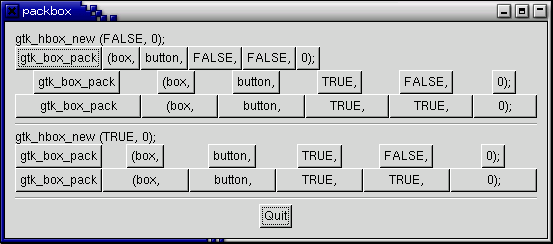
\includegraphics[height=50mm]{images/packbox1.png}
\end{center}
\end{figure}

Ahogy korábban a kódsorokat, most a \textit{widget}sorokat vesszük sorra a minél jobb megértés kedvéért.

\subsubsection{Méretarányos elhelyezés}

\begin{description}
 \item[\textit{expand} = \textit{false}, \textit{fill} = \textit{false}] A konténerben lévő elemek -- ahogy fentiekben fogalmaztunk -- nem akarnak egymás rovására helyet szerezni (\textit{epxand}), így a rendelkezésre álló vízszintes helyet nem is töltik ki, vagyis ezzel a megoldással az egész elemsorra nézve egyfajta balra (\textit{pack\_end} esetén jobbra) zártság alakítható ki.

\index{konténer!size allocation@\textit{size allocation}}
 \item[\textit{expand} = \textit{true}, \textit{fill} = \textit{false}] Az összkép -- az alatta található sor miatt -- kissé csalóka, mivel az elemek kissé rendezetlennek tűnnek, ugyanakkor arról van szó, hogy minden egyes elem megszerezte magénak -- a saját eredeti méretigényének arányában -- a rendelkezésre álló plusz helyet és az így allokált (\textit{size allocation}) térrészen belül középen helyezkedik el.

 \item[\textit{expand} = \textit{true}, \textit{fill} = \textit{true}] Az egyes elemek nem csak hogy kiterjeszkedtek (\textit{expand}) a korábban fel nem használt területre, de ki is töltik (\textit{fill}) azt, azaz annak terjedelmében rajzolják meg magukat.
\end{description}

Ahogy az az ábrából -- és talán a magyarázatból is -- kitűnik az \textit{fill} opció állításának semmi teteje anélkül, hogy az \textit{expand} be ne lenne kapcsolva, hisz e nélkül nincs semmilyen plusz terült, amire a \textit{widget} magát megnagyobbítva rajzolhatná.

\subsubsection{Homogén elhelyezés}
\index{GtkBox@\texttt{GtkBox}!tulajdonságok!homogeneous@\texttt{homogeneous}}
\index{GtkBox@\texttt{GtkBox}!gyerek tulajdonságok!fill@\texttt{fill}}
\index{GtkBox@\texttt{GtkBox}!gyerek tulajdonságok!expand@\texttt{expand}}

\begin{description}
 \item[\textit{expand} = \textit{true}, \textit{fill} = \textit{false}] A konténerben lévő elemek -- a már használt kifejezéssel élve -- nem akarnak egymás rovására helyet szerezni (\textit{epxand}), így a rendelkezésre álló vízszintes helyet nem is töltik ki, vagyis ezzel a megoldással az egész elemsorra nézve egyfajta balra (\textit{pack\_end} esetén jobbra) zártság alakítható ki.

\index{konténer!size allocation@\textit{size allocation}}
 \item[\textit{expand} = \textit{true}, \textit{fill} = \textit{true}] Az összkép -- az alatta található sor miatt -- kissé csalóka, mivel az elemek kissé rendezetlennek tűnnek, ugyanakkor arról van szó, hogy minden egyes elem megszerezte magénak -- a saját eredeti méretigényének arányában -- a rendelkezésre álló plusz helyet és az így allokált (\textit{size allocation}) térrészen belül középen helyezkedik el.
\end{description}

\subsection{Térköz}
\index{GtkBox@\texttt{GtkBox}!tulajdonságok!spacing@\texttt{spacing}}
\index{GtkBox@\texttt{GtkBox}!gyerek tulajdonságok!padding@\texttt{padding}}

Térköz megadására két lehetőség is kínálkozik a ha elemeket szeretnénk elhelyezni egy \textit{box}ban. Az egyik, hogy magának a konténernek állítunk be létrehozáskor -- vagy akár később -- \textit{spacing}et, vagy az egyes elemek hozzáadásakor adunk meg \textit{padding}et. Hogy mi a különbség a két eset között az alábbi ábra -- ahol az fenti blokkban az első, míg az alsó blokkban a második esetre látunk példát -- jól illusztrálja.

\vspace{12 pt}
\begin{figure}[H]
\begin{center}
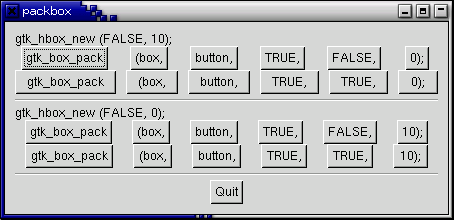
\includegraphics[height=50mm]{images/packbox2.png}
\end{center}
\end{figure}

\subsubsection{Tér az elemek között}
\index{GtkBox@\texttt{GtkBox}!tulajdonságok!spacing@\texttt{spacing}}

\begin{description}
 \item[\textit{expand} = \textit{true}, \textit{fill} = \textit{false}] Ez a példa nem mutatja igazán jól meg azt, hogy az elemek között jelenik meg az a térköz, amit a konténer létrehozásakor megadtunk.

 \item[\textit{expand} = \textit{true}, \textit{fill} = \textit{true}] Mivel itt mindkét érték \textit{true}, a \textit{widget}ek a rendelkezésre álló teret teljes egészében kihasználják maguk megrajzolására, eltekintve természetesen a közöttük megjelenő 10 pixel \textit{spacing}től. Érdemes külön megfigyelni a két szélső elemet, azoknak is az ablak széléhez közelebb eső részét a másik megoldással való összehasonlításhoz.
\end{description}

\subsubsection{Tér az elemek körül}
\index{GtkBox@\texttt{GtkBox}!gyerek tulajdonságok!padding@\texttt{padding}}

\begin{description}
 \item[\textit{expand} = \textit{true}, \textit{fill} = \textit{false}] A \textit{padding} megadásával a térköz nem az elemek között, hanem azok körül jelenik meg. Ez azt jelenti, hogy minden elem jobb és bal oldalán (\texttt{GtkVBox} esetén felül és alul) egyaránt jelentkezik a megadott térköz, ennek okán közöttük annak minimum (függően a \textit{fill} értékétől) a kétszerese.

 \item[\textit{expand} = \textit{true}, \textit{fill} = \textit{true}] Ez az az eset amikor igazán jól látható a \textit{widget}ek között és az azok mellett megjelenő térköz 2:1 aránya. Az előbb -- a szélső widgetek elhelyezkedésénél megfigyelteket -- most hasznosíthatjuk, ha észrevesszük itt a szélső \textit{widget}ek nem tudnak a konténer széléig kiterjeszkedni, lévén két oldalról ki vannak párnázva (\textit{pad}) 10-10 pixellel.
\end{description}

\section{A kód}

A fenti példaprogramok forrása, illetve azok eredetijei, a \textit{FLOSSzine}, valamint a \textit{GTK+} oldalain az alábbi linkeken érhetőek el:
\ \\\\
\url{http://www.flosszine.org/sources/gtk_packbox.c}\\
\url{http://library.gnome.org/devel/gtk-tutorial/2.17/x387.html}

\subsection{Fordítás és linkelés}

A korábbiakhoz hasonlóan az alábbi parancssorok segítségével fordíthatóak elemzett programjaink:

\lstccompile{gtk_packbox.c}{gtk_packbox}

\subsection{Futtatás}

Próbáljuk ezúttal a \texttt{./gtk\_packbox 1|2|3}, illetve a \texttt{./gtkmm\_packbox 1|2|3} parancsokkal abban a könyvtárban, ahol a fordítást elkövettük, ahol a paraméter a teszt sorszáma, abban a sorrendben, ahogy azokat itt is ismertettük (a 3. természetesen ráadás).

\subsection{Eredmény}

Ha netán úgy érezzük mégsem világos mi is történik, mikor és miért a konténerekbe pakolás kapcsán ne adjuk fel. Elsőre talán az egész mechanizmus jelentősége sem szembetűnő, ugyanakkor érdemes próbálkozni, azaz venni a forrást és játszani a különböző értékekkel (\textit{fill}, \textit{expand}, \textit{spacing}, \textit{padding}), illetve a létrehozott ablak átméretezésével.

%
%\chapter{Ablakok}
%\section{Bevezetés}
\index{GtkWindow@\texttt{GtkWindow}}
\index{GtkDialog@\texttt{GtkDialog}}

Ebben a részében a \textit{GTK}-ban létrehozható különböző ablaktípusok közös vonásait, valamint eltéréseit, illetve ezek okait vesszük sorra. Kitérünk egyrészről az egyes ablaktípusok létrehozásának sajátosságaira, azok \textit{widget}ekkel való feltöltésére, másrészről a felhasználó interakciók kezelésére, ezzel együtt az ablakok bezárásának módjaira is, szem előtt tartva természetese a \textit{C}, \textit{C++}, illetve \textit{Python} nyelvű változat azonosságait, különbözőségeit.

\subsection{\textit{Popup} és \textit{toplevel} ablakok}
\label{sec:windowtype}
\index{ablak!típus!popup}
\index{ablak!típus!toplevel}
\index{GtkWindow@\texttt{GtkWindow}!tulajdonságok!type@\texttt{type}}

A \textit{popup} ablakra, mint típusra ugyan ritkán lesz közvetlenül szükségünk, érdemes tudni, hogy a \textit{GTK} ebben a tekintetben két fajta ablakot különböztet meg. A \textit{popup} (felugró, felbukkanó) ablakokat, melyekre -- valamilyen speciális célt szolgáló saját készítésű \textit{widget}ektől eltekintve -- csak néhány példa létezik (\textit{menu}, \textit{tooltip}), valamint a \textit{toplevel} (legkülső, legfelső szintű) ablakokat, melyek csaknem minden \textit{GTK}-s, illetve saját fejlesztésű ablak alapjául szolgálnak. Ha tehát az ablakra, illetve a hozzá kapcsolódó fogalmakra gondolunk, többségében egy \textit{toplevel} ablakra gondolunk, és nem a \textit{popup}\footnote{Más eszközkészletek a ``popups'' gyűjtőfogalom alá sorolják a dialógusokat, a \textit{GTK} esetén azonban egy dialógus ablak mindig egy \textit{toplevel}} típusúakra, melyekről talán nem is feltételeznénk első ránézésre, hogy ablakok.

\index{GtkWindow@\texttt{GtkWindow}!tulajdonságok!type@\texttt{type}}
Az ablakkezelő ezt az információt használja fel annak eldöntésére, hogy az adott ablakot milyen kerettel, dekorációval lássa el, illetve hogy általánosságban menedzselje e ablakot. Utóbbi -- azaz a \textit{toplevel} ablakok -- esetben alapértelmezetten az ablakkezelő keretet, illetve a beállításoktól függően azon például bezáró, teljes mértre váltó, minimalizáló gombot jelenít meg. A \textit{popup} típusú ablakokat az ablakkezelő nemcsak hogy nem dekorálja, de nem is menedzseli azokat, következésképp tehát számos -- az ablakkezelő hatáskörébe tartozó -- funkció, mint amilyen például a minimalizálás, vagy a maximalizálás nem is érhető el. Bár kézenfekvő megoldásnak látszik a \textit{popup} típus arra, ha egy dekoráció nélküli ablakot készítsünk, mégse ezt tegyük, az ilyen típusú megjelenésbeli sajátosságok beállítására léteznek külön függvények.

\index{GtkBin@\texttt{GtkBin}}
Minden \texttt{GtkWindow} egyben konténer is, pontosabban fogalmazva egy \textit{GtkBin}, azaz tartalmazhat egy további elemet gyerekként, ami természetesen szintén lehet egy konténer, így biztosítva, hogy számos elemet helyezhessünk el az elkészített ablakon belül.

\subsection{\textit{Window} és \textit{dialóg}}
\index{GtkWindow@\texttt{GtkWindow}}
\index{GtkDialog@\texttt{GtkDialog}}
\index{GtkBox@\texttt{GtkBox}!függvények!pack\_end@\texttt{pack\_end}}
\index{GtkBox@\texttt{GtkBox}!függvények!pack\_start@\texttt{pack\_start}}

\label{par:dialogbox}
\index{ablak!típus!toplevel}
\index{GtkBox@\texttt{GtkBox}}
\index{GtkButtonBox@\texttt{GtkButtonBox}}
\index{GtkSeparator@\texttt{GtkSeparator}}
\index{GtkDialog@\texttt{GtkDialog}!belső elemek!action\_area@\texttt{action\_area}}
\index{GtkBox@\texttt{GtkBox}!függvények!pack\_start@\texttt{pack\_start}}
\index{GtkBox@\texttt{GtkBox}!függvények!pack\_end@\texttt{pack\_end}}
A \textit{window} típus -- azon belül is ahogy tárgyaltuk a \textit{toplevel window} -- közvetlen szülője a \textit{dialog} típusnak, számottevő különbség tulajdonképpen nincs is a kettő között. Egy \textit{dialog} nem más, mint egy olyan \textit{window}, melybe a \textit{GTK+} fejlesztői néhány hasznos elemet helyeztek el. Konkrétabban fogalmazva minden dialógba egy függőleges elrendezésű konténer \textit{widget} (\texttt{GtkBox}), abba pedig egy, a gombok elhelyezésére szolgáló konténer (\texttt{GtkButtonBox} típusú \texttt{action\_area}), valamint egy szeparátor (\texttt{GtkSeparator}) kerül, ebben a sorrendben mindkét esetben a konténer aljára helyezve\footnote{A \texttt{GtkBox} típus \texttt{pack\_end()} függvényét hívva.}. Ebből következik, hogy minden, amit egy dialógusba -- annak elkészült után -- tenni akarunk az a gombsor, valamint a vízszintes szeparátor fölött jelenik meg, függetlenül attól, hogy azt a \texttt{pack\_start()}, vagy a \texttt{pack\_end()} függvény segítségével helyezzük el a konténerben.

\index{GtkDialog@\texttt{GtkDialog}!belső elemek!content\_area@\texttt{content\_area}}
A \textit{dialog} típus tehát -- a szeparátor által -- függőlegesen ketté osztott \textit{window}, ahol az alsó rész (\texttt{action\_area}), ami általában a gombokat tartalmazza (pl.: Ok, Mégse, Súgó, \dots), a felső (\texttt{content\_area}) pedig azokat az elemeket tartalmazza, amik a felhasználói számára a szükséges akcióhoz (pl.: adatbevitel, hibaüzenet megjelenítése, \dots) szükséges.

\subsection{Modalitás}
\label{sec:windowmodal}

\index{ablak!modalitás}
\index{GtkWindow@\texttt{GtkWindow}!tulajdonságok!modal@\texttt{modal}}
A több ablakkal történő párhuzamos interakció tiltására szolgál a \textit{window} \textit{modal} tulajdonsága. Amennyiben egy ablak ``modális'' csak az abban az ablakban elhelyezkedő \textit{widget}ekbe történhet például bevitel, csak azokon váltódhat ki valamilyen felhasználó által kezdeményezett esemény. Ezt kihasználva biztosíthatjuk például, hogy egy adatbeviteli ablak\footnote{Ilyen lehet például a \textit{szerkesztés} menüpontok \textit{beállítások} almenüjének hatására megjelenő ablak.} bezárásáig ne változzon semmilyen, a felhasználó által módosítható, \textit{widget} tartalma a háttérben.

Modalitásnak két formáját különböztetjük meg. Egyrészről -- amiről eddig is szó esett -- a csak az applikációra vonatkozó modalitást, mely lehetővé teszi, hogy más applikációk ablakaihoz minden további nélkül hozzáférhetünk. Másrészről a teljes rendszerre érvényes modalitást, ahol a modális ablakon kívüli ablakokkal folytatott minden nemű felhasználó interakció tiltott. Ez utóbbi módszert csak a legszükségesebb esetben -- már ha van ilyen -- célszerű alkalmazni és az előbbi is csak akkor fogadható el felülettervezési szempontból, ha az applikáció egyéb részeihez való hozzáférés adatvesztést, vagy más komoly hibát okozna. Amennyiben mégis a modalitás mellett döntünk, ami nem ritka, hiszen az adatbevitelre, módosításra használt ablakok majd mindegyike ilyen, fontos egyértelművé tenni a felhasználó számára, hogy miként hagyhatja el azt az ablakot, ami korlátozza az applikáció más részeihez való hozzáférését. Egy ilyen menekülő útvonal biztosításának kézenfekvő módja lehet például egy \textit{Mégse} feliratú gomb.

\subsection{Tranziencia}
\label{sec:windowtransientfor}

\index{ablak!tranziencia}\index{GtkWindow@\texttt{GtkWindow}!tulajdonságok!transient-for@\texttt{transient-for}}
A dialógusok rendszerint ``tranziensek'' arra az ablakra, melyből származnak, azaz arra az ablakra melyen azt a műveletet váltottuk ki, aminek hatására a dialógus megjelent. Ezen beállítás alapján az ablakkezelő képes a dialógusunkat előtérben, a szülőablak fölött tartani\footnote{Helytelen beállítások esetén -- ha rosszul, vagy egyáltalán nem adjuk meg a szülőablakot -- előfordulhat, hogy egy újonnan létrehozott és megjelenített dialógusunk a már létező ablakok alatt, vagy között kerül megjelenítésre, ami felhasználói szempontból roppant zavaró}, valamint ha arra kérjük, akkor a szülő ablakhoz képest középen megjeleníteni (\ref{sec:windowpos}).

\index{GtkWindow@\texttt{GtkWindow}!tulajdonságok!destroy-with-parent@\texttt{destroy-with-parent}}
Ez a funkció azonban nem csak az ablakok helyes megjelenítéséhez szükséges, a megszüntetésükkor is hasznos, hiszen a \texttt{destroy-with-parent} tulajdonságon (\textit{property}) keresztül lehetőség van arra utasítani a \textit{GTK}-t, hogy egy ablak megszűnésekor azokat az ablakokat is szüntesse meg, melyek erre a szülőablakra nézve tranziensek. Ez leginkább akkor hasznos, hogy ha egy bizonytalan ideig létező ablakra szeretnénk tranziensek lenni\footnote{Erre lehet példa egy nem modális ablak, ami a programfutása során is megszűnhet}. Így nem kell törődnünk azzal, hogy ablakaink esetleg ``árván'' maradnak.\label{par:windowdestroywithparent}

\section{Használat}

\subsection{Létrehozás}
\index{GtkWindow@\texttt{GtkWindow}}
\index{GtkDialog@\texttt{GtkDialog}}

Mind a \texttt{GtkDialog}, mind pedig a \texttt{GtkWindow} típus létrehozása -- már ami formai részt illeti --, teljesen hasonló az összes többi \textit{widget}éhez, van azonban egy érdemi különbség, amire érdemes kitérni. Az ablakok -- igaz ez természetesen az összes többi \texttt{GtkWindow} típusból származó \textit{widget}re is (pl.: \texttt{GtkMessageDialog}, \texttt{GtkAboutDialog}, \dots) -- természetüknél fogva nem kerülnek bele más konténerbe, hiszen pont ezek azok a típusok, amik \textit{widget}eket tartalmaznak. Ellentétben azonban a többi típussal, ahol a referenciaszámlálás megoldja a problémát, itt a létrejött \textit{widget}ek felszabadításáról magunknak kell gondoskodnunk.

\subsubsection{Paraméterek}

A \texttt{GtkDialog} létrehozásában már valamivel nagyobb a különbség, függően attól, hogy \textit{GTK+}-t, vagy \textit{gtkmm}et használunk, bár így sem számottevő. Minkét esetben meg kell adnunk a címsor szövegét, valamint azt az ablakot, amire tranziensek kívánunk lenni. \textit{GTK+} esetén -- ahogy látszik -- lehetőségünk van \texttt{NULL} érték megadására, ami azt jelenti, hogy nem kívánunk ezzel a lehetőséggel élni. A \textit{gtkmm} is lehetséges ez, ha az alább látható konstruktort helyett azt hívjuk, amelyből hiányzik a \texttt{parent} paraméter.

\lsttriplesourcev
{sources/window_create.h}
{sources/window_create.hpp}
{sources/window_create.py}
{\textit{Window} létrehozása}
{lst:windowcreate}

\index{ablak!típus}
\index{ablak!típus!popup}
\index{ablak!típus!toplevel}
Ahogy arról szó esett (\ref{sec:windowtype}) a \textit{GTK} két típust különböztet meg -- a \textit{popup} és \textit{toplevel} \textit{window} -- melyek közül az előbbi olyannyira ritkán használt, hogy a \textit{C++} nyelvű változat esetén az alapértelmezett paramétere is van a típus konstruktorának, ahol a típus alapértelmezett értéke \textit{toplevel}.

\index{GtkWindow@\texttt{GtkWindow}!tulajdonságok!modal@\texttt{modal}}
A \textit{C}, illetve a \textit{Python} változat \texttt{flags} paramétere egyben tartalmazza a \textit{gtkmm} \texttt{modal} (\ref{sec:windowmodal}) és a \texttt{destroy-with-parent} (\ref{par:windowdestroywithparent}) értéket egy \textit{bitmask} értékben. Ez utóbbi beállítására ugyan van lehetőség \textit{gtkmm} esetén is, a \textit{C++} nyelvi eszközeinek korrekt használata mellett nemigen van szükség\footnote{Ha egy ablakra egy tranziens dialógust akarunk megjeleníteni, az nyugodtan lehet adattag, aminek megszüntetéséről az ablak destruktorában gondoskodhatunk.}.

\lsttriplesource
[numbers=none]
{sources/dialog_create.h}
{sources/dialog_create.hpp}
{sources/dialog_create.py}
{\textit{Dialog} létrehozása}
{lst:dialogcreate}

\subsubsection{Pozíció}
\label{sec:windowpos}
\index{ablak!pozíció}

Egy ablak képernyőn elfoglalt pozíciójának megadására alapvetően két lehetőség kínálkozik. Az egyik, ha előre -- még az ablak megjelenítése előtt -- megadjuk, a kívánt elhelyezkedést. Ehhez a \textit{GTK} annyiban tud segítségünkre lenni, hogy választhatunk néhány előre definiált elhelyezkedési pozíció közül, így nem szükséges a pixelben megadott koordináták kiszámítására időt és energiát pazarolni\footnote{Ami nem minden esetben kézenfekvő feladat, hiszen adott esetben nem csak a képernyő felbontásával, saját ablakunk méreteivel, de a szülőablak, vagy éppen a desktop szélesség és magasság értékeivel is foglalkozni kell.}.

\index{GtkWindow@\texttt{GtkWindow}!függvények!set\_position@\texttt{set\_position}}
\index{GtkDialog@\texttt{GtkDialog}!függvények!run@\texttt{run}}
\index{GtkWidget@\texttt{GtkWidget}!függvények!show@\texttt{show}}
A \texttt{set\_position} függvény még a megjelenítést megelőzően -- azaz \textit{window} esetén a \texttt{show}, \textit{daialog} esetén pedig a \texttt{run} meghívása előtt -- módunkban áll az alábbi elhelyezkedési sémák közül a megfelelőt kiválasztani.

\begin{description}
 \index{Gtk@\texttt{Gtk}!konstansok!WIN\_POS\_NONE@\texttt{WIN\_POS\_NONE}}
 \item[\texttt{WIN\_POS\_NONE}] Nincs befolyással a megjelenítést ablak pozíciójára nincs.

 \index{Gtk@\texttt{Gtk}!konstansok!WIN\_POS\_CENTER@\texttt{WIN\_POS\_CENTER}}
 \item[\texttt{WIN\_POS\_CENTER}] A megjelenítendő ablak a teljes képernyőhöz képest középen jelenik meg.

 \index{Gtk@\texttt{Gtk}!konstansok!WIN\_POS\_MOUSE@\texttt{WIN\_POS\_MOUSE}}
 \item[\texttt{WIN\_POS\_MOUSE}] A megjelenítendő ablak az egér aktuális pozíciója alatt jelenik meg.

 \index{Gtk@\texttt{Gtk}!konstansok!WIN\_POS\_ALWAYS@\texttt{WIN\_POS\_ALWAYS}}
 \item[\texttt{WIN\_POS\_CENTER\_ALWAYS}] A megjelenítendő ablak a teljes képernyőhöz képest középen jelenik meg és átméretezést követően is ott marad\footnote{A legtöbb esetben ez a választás nem szerencsés, lévén nem feltétlenül működik ez a mód minden ablakkezelő rendszer esetén.}.

 \index{ablak!tranziencia}
 \index{GtkWindow@\texttt{GtkWindow}!függvények!set\_transient\_for@\texttt{set\_transient\_for}}
 \index{Gtk@\texttt{Gtk}!konstansok!WIN\_POS\_CENTER\_ON\_PARENT@\texttt{WIN\_POS\_CENTER\_ON\_PARENT}}
 \item[\texttt{WIN\_POS\_CENTER\_ON\_PARENT}] A megjelenítendő ablak -- a \texttt{set\_transient\_for} függvénnyel beállított -- szülőjéhez képest középen jelenik meg.
\end{description}

\index{ablak!pozíció}
\index{GtkWindow@\texttt{GtkWindow}!függvények!move@\texttt{move}}
\index{GtkWindow@\texttt{GtkWindow}!tulajdonságok!gravity@\texttt{gravity}}
Ha úgy látjuk a fenti lehetőségek nem felelnek meg maradéktalanul céljainknak, akkor lehetőségünk van arra, hogy ablakunkat a kívánt pozícióra mozgassuk. Megjegyzendő, hogy ez a mozgatás csupán egy kérés az ablakkezelő felé, amit az figyelmen kívül is hagyhat. Az ablakkezelők jelentékeny része ezt meg is teszi amennyiben ezzel a módszerrel kívánjuk az ablak kezdeti pozícióját meghatározni, viszont honorálja kérésünket, ha az ablak korábban már megjelenítésre került. Az ablak elhelyezkedésének megadása \textit{x}, \textit{y} koordinátákkal történik egy választott referenciaponthoz képest, mely lehet az ablak bármely sarokpontja, az élek középpontja és az ablak középpontja egyaránt. A mozgatás maga a \texttt{move} függvénnyel történik, a referenciapontot pedig a \texttt{gravity} értéke határoz meg.

\index{GtkWindow@\texttt{GtkWindow}!függvények!get\_position@\texttt{get\_position}}
Egy ablak pozíciójának nem csak a beállítására, de lekérdezésére is szükség lehet, ugyanakkor ebben a tekintetben adott egy komoly megszorítás, amivel mindenképp szükséges számolni. A \texttt{get\_position} függvény által visszaadott értékek a már korábban említett módon függenek egyrészről a \texttt{gravity} értékétől, másrészről pedig az ablakkezelőtől. Elméletben, ha a visszakapott \textit{x}, illetve \textit{y} értéket átadnánk a \texttt{set\_position} függvények azt kellene tapasztalnunk, hogy az ablak egy helyben marad, gyakorlatban viszont azt tapasztalhatjuk, hogy az ablak valamennyit elmozdul. Ennek oka az ablakkezelő által az ablak köré rajzolt dekoráció, illetve annak geometriája, amit a \textit{GTK+} csak jó közelítéssel tud becsülni. Ez például akkor okozhat gondot, ha programunk ablakainak méretét és elhelyezkedését menteni szeretnénk, majd azt visszaállítanánk a következő futtatásnál. Érdemes tehát körültekintőnek lenni.

\subsubsection{Méret és arány}

A konténerek méretének meghatározásáról és elemeik (\textit{children}) elhelyezkedéséről leírtak (\ref{sec:packing}) a belső elrendezésük arányait átméretezéskor is megtartó ablakok kialakításakor válnak igazán fontossá.

\index{GtkWindow@\texttt{GtkWindow}!függvények!set\_default\_size@\texttt{set\_default\_size}}
\index{GtkWindow@\texttt{GtkWindow}!tulajdonságok!size-request@\texttt{size-request}}
\index{GtkWidget@\texttt{GtkWidget}!függvények!hide@\texttt{hide}}
\index{konténer!size request@\textit{size request}}
Egy ablak méretét, ha más erre vonatkozó beállítást nem teszünk -- épp úgy mint mint minden más konténerét -- a benne lévő elemek méretigény határozza meg, ugyanakkor lehetőség van ennek az alapértelmezés szerinti működésnek a módosítására. Egyrészről a \texttt{set\_default\_size} függvény révén, melynek megadható az ablak alapértelmezett vízszintes és függőeges mérete pixelben. Ennek hatása, hogy az ablak első megjelenítéskor\footnote{Egy esetleges eltüntetéskor \textit{hide} az ablak mérete úgymond mentésre kerül, azaz az alapértelmezett méret nem kerül újra alkalmazásra, ha az ablakot eltüntetjük \textit{hide}, majd újra megjelenítjük.} legalább ilyen méretű lesz. Ha azonban az ablakban tárolt \textit{widget}ek méretigénye azt indokolja, akkor a megadott szélesség és magasság értékeknél nagyon méretben kerül megjelenítésre. Ezt a működést természetesen a \textit{size request} megadása révén is elérhetnénk, de az alapértelmezett méret beállítása esetén a felhasználó csökkenteni tudja az ablak méretét, ha megadottak szerinti méretre nincs feltétlenül szükség.

\index{GtkBox@\texttt{GtkBox}!gyerek tulajdonságok!expand@\texttt{expand}}
\index{GtkBox@\texttt{GtkBox}!gyerek tulajdonságok!fill@\texttt{fill}}
\index{GtkWindow@\texttt{GtkWindow}!függvények!set\_resizable@\texttt{set\_resizable}}
\index{GtkWindow@\texttt{GtkWindow}!függvények!resize@\texttt{resize}}
Az ablak átméretezése kapcsán két felhasználói szempontból érdemleges kérdés merül fel. Az egyik, hogy engedjük-e az ablak átméretezését a felhasználónak. Erre a kérdésre adott válasz leginkább azon múlik, hogy mennyi időt kívánunk az ablak tervezésével tölteni, illetve mennyire van a felhasználónak igénye az átméretezésre. Ha időnk korlátos és valójában nincs szükség a méret megváltoztatására, akkor szerencsénk van, nyugodtan tilthatjuk ezt az interakció. Ha viszont ez nem lehetséges -- például azért, mert az alkalmazásunk főablakáról, vagy egy olyan dialógusról van szó, melyben egy lista jelenik meg, aminek hasznos lehet a lehető legtöbb helyet biztosítani --, akkor időt és energiát kell szálnunk az egyes widgetek viselkedésének megtervezésére. Át kell gondolnunk mely elemeknek foglalják el (\textit{expand}, \textit{fill}) azt a helyet, ami az átméretezés révén rendelkezésre áll majd. Egy-egy feleslegesen megnyúló \textit{widget} -- mondjuk egy teljes képernyőt elfoglaló beviteli mező, amibe mondjuk csak egy IP címet szeretnénk írni -- épp annyira szerencsétlenül mutat, mint amennyire zavaró az, ha hiába növeljük az ablak méretét, a lista, amiből több sort szeretnénk látni, mégsem nő. Ha mégis az átméretezés tiltása mellett döntenénk, akkor ezt a \textit{set\_resizable} függvény hívásával tudjuk elérni. A másik érdemleges kérdés a programból történő átméretezés, amire ugyan megoldható (\textit{resize}), de erősen ellenjavallt usability szempontból.

 \index{GtkWindow@\texttt{GtkWindow}!függvények!set\_geometry\_hints@\texttt{set\_geometry\_hints}}
A fentieknél is részletesebb beállítások a \textit{set\_geometry\_hints} függvénnyel tehetők meg. Az ablak minimális és a maximális vízszintes, illetve függőeges irányban külön-külön állíthatóak, ahogy az átméretezés lépésköze is, sőt az ablak méretarányának \footnote{$\mbox{szélesség} / \mbox{magasság}$ lebegőpontos számként adott értéke} (\textit{aspect ratio}) lehetséges legkisebb és legnagyobb értéke is megadható.

\subsection{Minimális példa}

Ennyi bevezető után lássuk egy olyan példát, ami a lehető legkevesebb kódsor mellet, még ha meglehetősen korlátozott funkcionalitás bíró, de működő alkalmazást eredményez. Az alábbi \textit{C}, \textit{C++}, illetve \textit{Python} nyelvű kód nem tesz egyebet, létrehoz egy ablakot, amit meg is jelenít azáltal, majd átadja a vezérlést a \textit{GTK}-nak azáltal, hogy futtatja a \textit{main loop}ot, 

\lsttriplesource
{sources/window_minimal.c}
{sources/window_minimal.cc}
{sources/window_minimal.py}
{Minimál példa \texttt{GtkWindow}hoz}
{lst:windowminimal}

A változatok bár egyformának tűnnek, néhány apróságban mégis eltérnek egymástól. Ezek egy része, mint a \texttt{window} változó deklarálásának helye, vagy paraméterezése, a programozási nyelv sajátosságaiból következik. Mások viszont, mint a \textit{main loop} futtatásának módja, illetve a függvény elnevezése már a nyelvi változat megalkotóinak belátásán műlik. A programok működése azonos, csupán a technikai megvalósításban vannak eltérések.

Ezekről korábban már szó esett, így itt ezeket nem részletezzük, inkább sorra vesszük miként vehetünk használatba egy frissen létrehozott ablakot, mit kell tennünk, ha elemeket szeretnénk elhelyezni az ablakban, ha vezérlő gombokkal szeretnénk látnánk el, majd a megjelenítést után a felhasználó interakciókat szeretnénk követni, illetve azokra reagálni.

\subsection{Tartalmi elemek}

\index{GtkBin@\texttt{GtkBin}}
Egy ablak típusa szerint nem más, mint egy konténer, pontosabban fogalmazva egy \texttt{GtkBin} (\ref{sec:bin}), amibe további elemeket tehetünk. Praktikusan ez az elem egy újabb konténer, rendszerint egy \texttt{GtkBox}. A \texttt{GtkDialog} esetén, mint azt a korábbiakban (\ref{par:dialogbox}) kifejtettük, a konténerbe helyezett \texttt{GtkBox} már adott.

Az így egy ablakba kerülő \textit{widget}ekre nem csak abban az értelemben tekintünk csoportként, hogy mindegyikük szülője -- \textit{toplevel widget} szinten -- ugyanaz az ablak, de vannak bizonyos tulajdonságok, melyek ugyan konkrétan a \textit{widget}re vonatkoznak, de összefüggésben állnak az ablak más \textit{widget}einek bizonyos tulajdonságaival, de mindig csak az azonos ablakban lévő más \textit{widget}ekéivel, vagyis erre csoport nézve zártak.

\subsubsection{Fókusz \textit{widget}}
\label{sec:widgetfocus}

\index{ablak!típus!toplevel}
\index{ablak!típus!popup}
\index{fókusz!billentyűzet}
Egy adott ablakban\footnote{Itt ablak alatt a \textit{toplevel} és nem a \textit{popup} ablakokat értjük.} egy adott pillanatban legfeljebb egy olyan \textit{widget} lehet, melyen fókuszban (\textit{keyboard focus}) van. Ha van ilyen \textit{widget}, akkor minden -- az ablak által fogadott -- billentyűzet esemény (billentyű lenyomása, felengedése, \dots) hozzá kerül továbbításra. Így érthető is, hiszen ha például gépelünk valamit a billentyűzeten, akkor annak eredményét értelemszerűen csak egy beviteli mezőben  szeretnénk látni.

\index{GtkEntry@\texttt{GtkEntry}}
\index{GtkTextView@\texttt{GtkTextView}}
\index{GtkContainer@\texttt{GtkContainer}}
\index{GtkContainer@\texttt{GtkContainer}!függvények!set\_focus\_chain@\texttt{set\_focus\_chain}}
A \textit{widget}ek többsége valamilyen látható módon is jelzi azt az állapotot, hogy aktuális fókuszban van. Ez az szövegbevitelre szolgáló \textit{widget}ek (\texttt{GtkEntry}, \texttt{GtkTextView}, \dots) esetén abban nyilvánul meg, hogy a kurzort látjuk villogni a beviteli mezőben, egyéb esetekben ezt egy vékony fekete keret jelzi. A fókusz egyik \textit{widget}ről a másikra történő mozgatására a szokások módszer, azaz a tab, illetve a kurzormozgató billentyűk használhatóak. Az egyes \textit{widget}ek között történő váltás is testre szabható a \texttt{GtkContainer} \texttt{set\_focus\_chain} függvényével, de erre valóban ritkán lehet szükség.

\begin{figure}[H]
\begin{center}

\includegraphics[height=15mm]{images/widget-keyboard-focus.png}
\caption{Billentyűzet fókusz jelzése a \textit{widget}en}
\end{center}
\end{figure}

\index{GtkWidget@\texttt{GtkWidget}!tulajdonságok!can-focus@\texttt{can-focus}}
\index{GtkWidget@\texttt{GtkWidget}!függvények!grab\_focus@\texttt{grab\_focus}}
Az egyes \textit{widget}ekre külön-külön engedhető, vagy tiltható, hogy fókuszba kerülhessenek, a \textit{can-focus} tulajdonság állításával. Az egyes \textit{widget}típusok esetében az alapértelmezés szerinti érték rendszrint megfelel a céljainknak\footnote{Ez az érték egy \texttt{GtkEntry} esetén igaz, míg egy \textit{Gtkabel} esetén hamis alapértelmezés szerint.}. Ha kódból szeretnénk átmozgatni a fókuszt az egyik \textit{widget}ről a másikra, vagy csak azt kívánjuk elérni, hogy az ablak megjelenítésekor legyen olyan \textit{widget} ami fókuszban van, akkor a \texttt{grab\_focus} függvényt kell alkalmaznunk, aminek előfeltétele a \textit{can-focus} tulajdonság igaz értéke, azaz fókuszálhatónak kell lennie, ami viszont bizonyos \textit{widget}ek (pl.: \texttt{GtkFrame}) esetén nem lehetséges.

\subsubsection{Alapértelmezett \textit{widget}}

\index{GtkDialog@\texttt{GtkDialog}
\index{gomb!jóváhagyó}
\index{gomb!ok}
\index{GtkWidget@\texttt{GtkWidget}!tulajdonságok!has-default@\texttt{has-default}}
A \texttt{GtkWindow} estén -- amit rendszerint olyan ablakhoz használunk aminek nincsenek gombjai -- ritkábban, míg \texttt{GtkDialog}} esetén csaknem mindig használt tulajdonság az alapértelmezett \textit{widget}. Ez ellentétben a fókusszal, ami inkább egy logikai tulajdonság, a felületre nincs, csak a működésre van hatással. Egy ablakon belül -- nevéből is következően -- legfeljebb egy olyan \textit{widget} lehet, mely rendelkezik ezzel a tulajdonsággal, ez rendszerint a dialógus jóváhagyó (\textit{affirmative}) gombja, jellemzően az \textit{Ok} gomb. 

\begin{figure}[H]
\begin{center}

\includegraphics[height=15mm]{images/button-affirmative.png}
\caption{Gombok szokások sorrendje egy dialógusban}
\end{center}
\end{figure}

\index{billentyű!tab}
\index{billentyű!enter}
\index{GtkEntry@\texttt{GtkEntry}}
\index{GtkTextView@\texttt{GtkTextView}}
\index{GtkWidget@\texttt{GtkWidget}!tulajdonságok!can-default@\texttt{can-default}}
\index{GtkWidget@\texttt{GtkWidget}!tulajdonságok!has-default@\texttt{has-default}}
\index{GtkEntry@\texttt{GtkEntry}!tulajdonságok!activates-default@\texttt{activates-default}}
Hatása abban áll, hogy az alapértelmezett \textit{widget} -- vagyis ami esetén a \texttt{has-default} tulajdonság értéke igaz -- aktiválódik akkor, ha egy egysoros beviteli mező van fókuszban (\texttt{GtkEntry}) és akkor \textit{Enter}t nyomunk, ez is csak akkor, ha az \texttt{GtkEntry} \texttt{activates-default} tulajdonsága szintén igaz értékű. Többsoros beviteli mező (\texttt{GtkTextView}) esetén ez nem működőképes, hiszen ott az \textit{Enter} lenyomása soremelést jelent. Az alapértelmezett \textit{widget}nek a billentyűzetről való használat kényelmesebbé tételében van szerepe, hiszen ha minden szükséges mezőt kitöltöttünk egy dialógusban, akkor nem kell a megfelelő gombig -- egérrel, vagy \textit{Tab} billentyű(k) lenyomásával -- elnavigálnunk, csak egyszerűen az \textit{Enter} leütésére aktiválódik az alapértelmezett \textit{widget}.

Ahhoz, hogy egy \textit{widget} egyáltalán számításba kerüljön, mint potenciális alapértelmezett \textit{widget}, ahhoz először a \texttt{can-default} tulajdonságának kell igaznak lenni, ilyen \textit{widget} több is lehet egy ablakon belül, melyek közül aktuálisan alapértelmezetté \texttt{GtkWidget} osztály \texttt{garb\_default} függvényével tehetünk egyet, így annak \texttt{has-default} értékkel igazzá válik, míg az ablak korábbi alapértelmezett \textit{widget}e, már ha volt ilyen, esetén a tulajdonság értéke természetesen hamis lesz.

\subsection{Vezérlő elemek}
\label{sec:windowvsdialog}

Amennyiben a szükséges tartalmi elemeket elhelyeztük az ablakban, a vezérlő elemekkel is hasonlóan kell eljárnunk. A különböző célokra használt ablakok különböző vezérlő elemeket kívánnak meg, amik az egyes típusokként erős hasonlóságot mutatnak. Egy főablak csak kivételes esetekben tartalmaz az eddigiekben tárgyalt gombokat, a vezérlés általában menükkel, a \textit{toolbar}on elhelyezett gombokkal történik (\ref{fig:windowprimary} ábra).

\includetwingraphics
{Főablak}
{window-primary.png}
{windowprimary}
{Dialógus}
{window-dialog.png}
{windowdialog}
{Tipikus ablakszerkezetek\cite{gnomehig}}
{windowtypes}

A főablakból nyíló különböző célú ablakok, melyek például egy adott elem tulajdonságainak beállítására, egy bonyolultabb funkció lépésenként történő megvalósítására, az alkalmazás egészének konfigurálására, egy folyamat nyomkövetésére, esetleg a felhasználó informálására, figyelmeztetésére szolgálnak, közvetlenül, vagy közvetve a \texttt{GtkDialog} típusból szármáznak, saját gombsorral látjuk el őket. Tipikus példa erre egy elem tulajdonságainak szerkesztésére használt dialógus (\ref{fig:windowdialog} ábra).

\subsubsection{\texttt{GtkDialog}}
\label{sec:dialogbuttonadd}
\index{GtkDialog@\texttt{GtkDialog}}

A \textit{C}, illetve a \textit{Python} nyelvű változat mutat némi különbözőséget a \textit{C++} változathoz képest a gombok hozzáadásának mikéntjében. Előbbiek esetén ugyanis több gombot is hozzáadhatunk egyszerre a dialógoshoz, egymás után sorolva a \texttt{button\_text} és a \texttt{response\_id} paramétereket. A paraméterlistát a \textit{C} változat esetén \texttt{NULL} értékkel kell zárnunk, különben változatos programhibákkal fogunk szembesülni, erre a \textit{Python} esetén nincs szükség, mivel itt a hívott fél tisztában van az átadott paraméterek számával.

\lsttriplesource
[numbers=none]
{sources/dialog_button_add.h}
{sources/dialog_button_add.hpp}
{sources/dialog_button_add_init.py}
{Gombok hozzáadása \texttt{GtkDialog}hoz}
{lst:dialogbuttonaddh}

\index{GtkStockId@\texttt{GtkStockId}}
A választott nyelvi változattól függetlenül igaz, hogy a \texttt{button\_text} paramétere vagy az általunk vágyott felirat szövege lehet, vagy egy \textit{stock ID} (\textit{Ok} gomb esetén például \texttt{GTK\_STOCK\_OK}).

\begin{figure}[H]
\begin{center}

\includegraphics[height=13mm]{images/button-alternate.png}
\caption{Egy tipikus gombsor}
\end{center}
\end{figure}

Egy fenti elrendezésű -- amúgy meglehetősen szokványos -- gombsor az alábbi kódrészletekkel hozható létre az egyes nyelvek esetén. Az eltérés nem számottevő, nem tartalmaz semmilyen olyan különbözőséget, ami a korábbiakban már ne került volna ismertetésre.

\lsttriplesource
[numbers=none]
{sources/dialog_button_add.c}
{sources/dialog_button_add.cc}
{sources/dialog_button_add.py}
{Tipikus gombsor hozzáadása \texttt{GtkDialog}hoz}
{lst:dialogbuttonadd}

\subsubsection{\texttt{GtkMessageDialog}}
\label{sec:messagedialog}
\index{GtkMessageDialog@\texttt{GtkMessageDialog}}

Létezik a \texttt{GtkDialog} típusnak egy -- a gombok hozzáadása szempontjából érdekes sajátossággal bíró -- specializált változata, melyet a felhasználóval történő kommunikáció céljaira használunk, s mely ennek megfelelően rendszerint csak az üzenet szövegét, illetve a válasz megadásához szükséges vezérlő elemeket tartalmazza.

\includetwingraphics
{Információs üzenetablak}
{message-dialog-information.png}
{messagedialoginformation}
{Hiba üzenetablak}
{message-dialog-error.png}
{messagedialogerror}
{Tipikus üzenetablakok}
{messagedialogtypes}

Az ábrákon látható dialógusokat -- a szövegezéstől eltekintve -- csak típusuk különbözteti meg egymástól. A bal oldali (\ref{fig:messagedialoginformation}) egy információs ablak, míg a jobb oldali (\ref{fig:messagedialogerror}) egy hibadialógus. Az egyik szembeötlő különbség az ablakok között az ikon, amit az üzenetablak típusa határoz meg. A fenti két típuson kívül még két saját ikonnal rendelkező típus (\textit{question} és \textit{warning}) létezik, illetve készíthetünk ikon nélküli változatot, aminél módunk van saját ikon megadására.

Az üzenetablak típus eltérése, vagy inkább specialitása a \texttt{GtkDialog} típushoz képest nem csak a típus megadásának lehetőségére korlátozódik. A kifejezetten a szoftver és a felhasználó közötti ``üzenetváltás'' célját szolgáló \textit{widget} rendelkezik beépített elemekkel az üzenet megjelenítésére. A felhasználóval közölni kívántakat egy elsődleges és egy másodlagos (\texttt{primary-text}, \texttt{secondary-text}) részre bonthatjuk, ahol az előbbi egy rövid, csak a helyzet leglényegesebb elemit tartalmazó, egy mondatos összefoglalója a közölni kívánt információnak, vagy a javasolt kívánt műveletnek, míg az utóbbi ennek mélyebb, részletekbe menő kifejtése leírása, ami tájékoztatja a felhasználót a felmerült helyzet okairól, esetleges mellékhatásairól. Az esetek többségében a felhasználónak már az elsődleges szöveg elolvasását követően meg kell tudni hoznia döntését, a másodlagos szöveg a döntés alátámasztására, az esetleges kétségek eloszlatására szolgál.

A harmadik specialitás -- a gombok felhelyezésének mikéntje -- a vezérlő elemek szempontjából is említésre méltó. Azzal együtt, hogy \textit{dialog} típusnál ismertetett módszer az öröklődés okán természetesen itt is használható, mivel azonban a leggyakrabban használt gombkombinációk száma erősen korlátos, így ezek közül létrehozáskor választhatunk. Lehetséges értékek eredményeként vagy egyedüliként a \textit{Bezárás}, \textit{Ok}, \textit{Mégse} gombok, vagy a \textit{Ok}/\textit{Cancel}, \textit{Igen}/\textit{Nem} párosok kerülnek a dialógusra.

\lsttriplesource
[numbers=none]
{sources/message_dialog_create.h}
{sources/message_dialog_create.hpp}
{sources/message_dialog_create.py}
{\textit{MessageDialog} létrehozása}
{lst:messagedialogcreate}

 \index{GLib@\texttt{GLib}!makrók!G\_GNUC\_PRINTF@\texttt{G\_GNUC\_PRINTF}}
A \textit{C}, illetve a \textit{Python} nyelvű változatok, ellentétben a \textit{C++}-os megvalósítással nem egyetlen paraméterként várják az üzenetablak elsődleges szövegét, hanem egy \texttt{printf}-stílusú formátumleírót és az annak megfelelő paramétereket vesznek át. Ennek típusbiztosságáról a \textit{C} változat esetén a \texttt{G\_GNUC\_PRINTF} makró gondoskodik, már amennyiben a \textit{GNU C} fordítót használjuk. Ebben az esetben fordítási idejű figyelmeztetést kapunk ha paramétereink nem felelnek meg a formátumleíróban megadottaknak.

\subsection{Megjelenítés}

Több lehetőség kínálkozik, ha egy ablakot, illetve annak tartalmát szeretnénk megjeleníteni. Használhatjuk egyrészről, a \texttt{GtkWidget}, a \texttt{GtkWindow}, illetve a \texttt{GtkDialog} típus által adott módszereket.

\subsubsection{\texttt{GtkWidget}}

\index{GtkWidget@\texttt{GtkWidget}!függvények!show@\texttt{show}}
\index{GtkWidget@\texttt{GtkWidget}!függvények!show\_all@\texttt{show\_all}}
A korábban már tárgyalt \texttt{show} függvényt, ami megjeleníti a \textit{window}t, de csak a \textit{window}t, annak gyerekeit nem. Lévén a \textit{window} egy konténer típus, helyezhetünk el további \textit{widget}eket benne, amiknek a megjelenítéséről vagy már korábban gondoskodnunk kell -- mondjuk egy \texttt{show} hívással --, vagy megtehetjük a szülő és az összes gyerek megjelenítését egyszerre a \texttt{show\_all} függvénnyel.

\subsubsection{\texttt{GtkWindow}}

\index{GtkWindow@\texttt{GtkWindow}!függvények!present@\texttt{present}}
Egy ablak esetén nem csupán a puszta megjelenítés lehet szempont, hanem az is, hogy a felhasználó az ablakot észre is vegye. Ez az estek túlnyomó többségében adott, hiszen valamilyen felhasználói interakció révén jelenik meg az új ablak. Ha viszont nem erről van szó akkor szükséges lehet az megjelenítésen túl más ablakok általi takarás megszüntetésére, a tálcáról való felhozatalra, az aktuális desktopra  történő mozgatásra, a fókusz (\ref{sec:widgetfocus}) átadására, mely műveletek mind függhetnek mind a platformtól, mind az ablakkezelőtől, mind pedig a felhasználói beállításoktól. Erre használható a \texttt{present} függvény. Kezeljük azonban kellő óvatossággal ezt a függvényt, hiszen mindannyian bosszankodtunk már egy kellő indok nélkül, váratlanul megjelenő ablak miatt.

\subsubsection{\texttt{GtkDialog}}

\index{main loop}
\index{GtkDialog@\texttt{GtkDialog}!függvények!run@\texttt{run}}
\index{GtkWindow@\texttt{GtkWindow}!tulajdonságok!modal@\texttt{modal}}
Egy \textit{window} típusú ablak esetén -- mivel jellemzően nincsenek az ablakon gombok és nem modálisak -- nincs igazán szükségünk arra, hogy -- a kód futásának szempontjából helyben -- kivárjuk a felhasználó reakciót. A \textit{dialog} típus ezzel szemben általában egy felhasználói interakció révén jelenik meg (pl.: egy elem tulajdonságait, vagy az applikáció beállításait szerkesztő ablak) és jelentős részben valamilyen döntés elé állítja a felhasználót (különösen igaz ez az üzenet ablakoknál, ahol kérést teszünk fel), melynek eredményéről szeretnénk értesülni. A \texttt{GtkDialog} típus \texttt{run} függvénye -- ahogy azt a következőekben (\ref{sec:dialogresponse}) részletesen is tárgyaljuk -- pontosan ezt a célt szolgálja. Egyrészről várakozik a felhasználó interakció -- amihez természetesen szükséges a \textit{main loop} futtatása -- majd visszatérési értékként az ablak ``futtatásának'' eredményét, vagyis a kiválasztott vezérlő elem -- az ablak elkészítésekor megadott -- \textit{response id}-t adja vissza. Mint látható, a függvény nem kifejezetten a dialógus megjelenítését szolgálja, az hasznos mellékhatásként mégis megtörténik.

\subsection{Bezárás}

A \textit{window} tehát leginkább a bezárás kapcsán állít kihívást elénk, melyet függően attól, mit szeretnénk elérni annak hatására, hogy a felhasználó az ablak bezárását kezdeményezte, több lehetséges megoldás, az egyes megoldásokra, pedig több módszer is kínálkozik.

\subsubsection{Blokkolás}

Kezdjük a legegyszerűbbnek látszó esettel, vagyis azzal, hogy semmilyen hatása ne legyen annak ha felhasználó az ablak bezárását kezdeményezi. Nyilván megfontolandó, hogy ezt tegyük, hiszen a felhasználó sem véletlenül akarja, amit akar, de ha mondjuk azt szeretnénk kikényszeríteni, hogy a főablakunkból csak a Fájl menüpont ``Kilépés'' almenüpontjára kattintva lehessen bezárni, akkor ez egy lehetséges megoldás\footnote{Ne becsüljük azonban alá se a felhasználói találékonyságot, se a felhasználói környezetek változatosságát. Semmiképp ne hagyatkozzunk arra, hogy egy adott módszer a felhasználó számára véleményünk szerint nem érhető el.}.

A feladat megoldása a korábban már tárgyalt \textit{delete-event} szignál kezelésében rejlik. Ahogy arról szó esett ez a szignál váltódik minden ablakon (\textit{toplevel window}), illetve minden az ablakban lévő \textit{widget}en, mikor a felhasználó az ablak bezárását kezdeményezi. A szignál két külön említésre is méltó sajátossággal is rendelkezik:

\begin{enumerate}
 \item A szignált kezelni kívánó függvénynek egy \textit{bool} értékkel kell visszatérnie, ami azt jelzi a \textit{GTK} felé, hogy az adott függvény kezelte-e az eseményt, egyszersmind nincs szükség a további kezelő függvény meghívására. A \textit{GTK} következésképp addig hívja sorra az szignálra ``feliratkozott'' függvényeket (\textit{signal handler}) -- köztük ha van ilyen, akkor az alapértelmezett szignálkezelő függvényt (\textit{default signal handler}) amíg egyikük \textit{true} értékkel nem tér vissza.
 \item Ha minden ilyen függvény \textit{false} értékkel tér vissza, azaz a szignál további propagálását kéri a \textit{GTK}-tól, akkor konkrétan a \texttt{delete-event} esetében a \textit{GDK} alapértelmezett eseménykezelője (\textit{default event handler}) fut le, ami meghívja az ablak destruktorát.
\end{enumerate}

Fentiek alapján ahhoz, hogy megelőzzük az ablak bezárását -- vagyis hogy ne történjen semmi -- el kell érnünk, hogy az alapértelmezett eseménykezelő ne hívódjon meg, azaz az általunk felkötött szignálkezelő \textit{true} értékkel kell hogy visszatérjen, jelezve azt, hogy az eseményt kezeltük, a további szignálkezelő függvények meghívására nincs szükség. Ebben az esetben ez azt is jelenti, hogy az alapértelmezett eseménykezelő sem hívódik meg. Ehhez definiálnunk kell a szignálkezelő  függvényeket, ami a korábbi (\lstref{lst:windowminimal}\footnote{A sorszámozás az eredeti példába való beillesztés pontját mutatja.}) példát kiegészítve az alábbihoz hasonló módon tehetünk meg,

\lsttriplesource
[firstnumber=2]
{sources/window_persistent_callback.c}
{sources/window_persistent_callback.cc}
{sources/window_persistent_callback.py}
{Szignálkezelő függvény perzisztens ablakhoz}
{lst:windowpersistentcallback}

majd ezeket a függvényeket a \texttt{delete-event} szignálra be is kell kötnünk\footnote{A sorszámozás az eredeti példába való beillesztés pontját mutatja.}.

\lsttriplesource
[firstnumber=12]
{sources/window_persistent_connect.c}
{sources/window_persistent_connect.cc}
{sources/window_persistent_connect.py}
{Szignálkezelő függvény bekötése perzisztens ablakhoz}
{lst:windowpersistentconnect}

Ha az adott szignál alapértelmezett szignálkezelő függvénnyel is rendelkezik -- ami a \textit{widget} osztály-leírójában kerül megadásra -- és magunk akarjuk a szignált kezelni, akkor szükségessé válik, hogy a saját kezelő függvényünk még az alapértelmezett előtt hívódjék meg, ami további praktikák bevetését igényli, amiről egy másik részben esett részletesebben szó.

\index{Gtk@\texttt{Gtk}!függvények!true@\texttt{true}}
\index{Gtk@\texttt{Gtk}!függvények!false@\texttt{false}}
Ha a saját szignálkezelő függvény írását kissé túlzónak találjuk egy olyan egyszerű feladat ellátására, mint egy \textit{true} értékkel való visszatérés, akkor nem tévedünk, sőt a \textit{GTK+} fejlesztői is gondoltak erre és megalkották a \texttt{gtk\_true}, illetve a \texttt{gtk\_false} nevű függvényeket, melyek semmi egyebet nem tesznek, mint a nevüknek megfelelő értékkel térnek vissza, így a fenti példa szignálkezelő függvényei elhagyhatók, hiszen azok \textit{GTK+} által adott -- ekvivalens funkciójú -- függvényekkel helyettesíthetőek.

\lstinputsource
[language=C]
{sources/window_persistent_simple.c}
{Egyszerűsített szignálkezelő függvény bekötése}
{lst:windowpersistentsimple}

\subsubsection{Eltüntetés}

Folytassuk másodikként azzal az eshetőséggel, ha el szeretnénk tüntetni az ablakot, aminek a bezárását a felhasználó kezdeményezte. Az előző szituációhoz hasonlóan most is több módszer adódik a feladat megoldására.

\index{GtkWidget@\texttt{GtkWidget}!függvények!hide@\texttt{hide}}
\index{GtkWidget@\texttt{GtkWidget}!szignálok!delete-event@\texttt{delete-event}}
A fent tárgyalt perzisztens ablakot eredményező szignálkezelők (\lstref{lst:windowpersistentcallback}) ismeretében a legnyilvánvalóbb megoldás, hogy még mielőtt visszatérnénk az adott függvényekből a \texttt{hide} függvény segítségével eltüntetjük az adott ablakot. A megoldás jó és működőképes megoldás lehet, ugyanakkor számolnunk kell azzal, hogy az ablak csak eltűnik, de nem feltétlenül semmisül meg. A már korábban is használt minimális példa azon kiegészítését is figyelembe vesszük, ahol a \texttt{delete-event} szignálra a \textit{main loop} futását megszakító függvényt hívjuk, akkor azt fogjuk tapasztalni, hogy az ablakunk eltűnik ugyan, de a mögöttes működés már nagyban attól függ a két implementációt (\lstref{lst:windowpersistentcallback}) miként vontuk össze. Ha a saját szignálkezelő függvényünket kötjük be előbb a \texttt{delete-event} szignálra, akkor az -- a visszatérési értéke révén -- leállítja a szignál további kezelését, vagyis a szignálkezelő függvények sorának meghívását is, így az ablak a saját kezelő függvényünk (\texttt{on\_delete\_event}), a \texttt{hide} hívással kiegészítve eltünteti az ablakot, de a következő szignálkezelő -- ami kiléptetné a \textit{main loop}ot -- már nem hívódik meg. Ha a felkötés sorrendje fordított, akkor előbb kilép a \textit{main loop} és csak ezután hívódik meg saját függvényünk, ami egyrészről elrejti az ablakot, másrészről blokkolja a további kezelést, aminek végső soron nem lehet hatása, hiszen a \textit{main loop} már kilépett.

Amennyiben a célunk csupán az ablak eltüntetése egyszerűbben is elérhetjük ugyanezt, hiszen a \texttt{hide} függvény közvetlenül -- pontosabban egy beépített \textit{GTK+} keresztül -- is beköthető a \texttt{delete-event} szignálra. Ezt kényelmi funkciót a \textit{gtkmm} esetén elveszítjük -- hasonlóan az előző példához --, mivel az általunk használni kívánt szignálkezelő függvény deklarációja nem egyezik meg az előírttal, így tehát ezt a ``kényelmet'' a típusbiztosság oltárán fel kell áldozni.

\lstinputsource
[language=C]
{sources/window_hide_on_delete_event_simple.c}
{Egyszerűsített szignálkezelő függvény bekötése}
{lst:windowpersistentsimple}

Ha nem ragadunk le a könnyen érthető, ám nem túl életszerű minimális példánknál, akkor az mondható el, hogy ablakokat -- legyenek azok \texttt{GtkWindow}, vagy \texttt{GtkDialog} típusúak --, valamilyen felhasználói interakcióra reagálva hozunk fel, valamilyen kezelő függvényben. Az bezáráskori elrejtés akkor lehet hasznos számunkra, ha nem akarjuk újra és újra elkészíteni az ablakot az adott felhasználói műveletre. Erre lehet példa mondjuk egy névjegy (\textit{about}) ablak, aminek a tartalma nem változik a program futása során, így azt az alkalmazás indulásakor, vagy az első megtekintéskor létrehozzuk, utána már elegendő csak elrejteni, vagy újra megjeleníteni. Másik példa lehet egy státusz jellegű információkat megjelenítő ablak, amiben úgymond gyűjteni tudjuk az adatokat és ha a felhasználó be is zárja az ablakot, mi az elrejtés után az adatgyűjtést és az ablak tartalmának frissítését tovább fojtatjuk, majd az újbóli megjelenítéskor már a naprakész információk jelennek meg.

\subsubsection{Megszüntetés}

\index{GtkWidget@\texttt{GtkWidget}!szignálok!delete-event@\texttt{delete-event}}
Mint az a fentiekből már kiderült -- függetlenül attól, hogy \texttt{GtkWindow}, \texttt{GtkDialog}, vagy ezekből származó típusokról van-e szó --, a \textit{delete-event} szignál kiváltódását -- ha egyebet nem teszünk -- az ablak destruktorának meghívás fogja automatikusan követni, ami az esetek túlnyomó többségében meg is felel a céljainknak.

\subsection{Eseménykezelés}
\label{sec:dialogresponse}

\subsubsection{Szinkron}

A \texttt{GtkDialog} és a \texttt{GtkWindow} típusok közötti eltérések (\ref{sec:windowvsdialog}) közül a legszámottevőbb -- mivel ehhez tartozik a legtöbb beépített szolgáltatás --, a vezérlő elemek, azaz a gombok kezelése. A \texttt{GtkDialog} nem csupán arra ad lehetőséget, hogy a gombokat egy erre a célra készült konténerbe helyezzük el -- ezt magunk is megtehetnénk minden különösebb erőfeszítés nélkül --, hanem az ezeken végzett felhasználói interakciókat is egyszerűen nyomon követhetjük. Választhatunk az adott (kód)környezetben számunkra kényelmesebb -- szinkron, illetve aszinkron eseménykezelés közül. Előbbi esetén helyben\footnote{Az ablak létrehozásának helyén.} tudjuk kezelni az eseményeket, utóbbi viszont eseménykezelő függvények megírását és bekötését teszi szükségessé.

\lsttriplesource
{sources/dialog_minimal.c}
{sources/dialog_minimal.cc}
{sources/dialog_minimal.py}
{Minimál példa \texttt{GtkDialog}hoz}
{lst:dialogminimal}

\index{main loop}
\index{GtkDialog@\texttt{GtkDialog}!függvények!run@\texttt{run}}
\index{GtkDialog@\texttt{GtkDialog}!szignálok!response@\texttt{response}}
\index{GtkWidget@\texttt{GtkWidget}!szignálok!unmap@\texttt{unmap}}
\index{GtkWidget@\texttt{GtkWidget}!szignálok!destroy@\texttt{destroy}}
\index{GtkWidget@\texttt{GtkWidget}!szignálok!delete-event@\texttt{delete-event}}
A \texttt{run} függvény (\ref{dialogminimalc:dialogrun}.) egyrészről függvényeket köt be a szükséges szignálokra (\texttt{response}, \texttt{unmap}, \texttt{delete-event}, \texttt{destroy}), majd egy saját \textit{main loop}ot futtatásán belül kezeli az említett eseményeket. Ha ezek közül bármelyik bekövetkezik, akkor a \textit{main loop} futása megszakad, és a \texttt{run} függvény a megfelelő értékkel visszatér. Ennek kezelése tipikusan egy \texttt{if}, vagy egy \texttt{switch} szerkezeten belül történik.

Ha a fenti minimális példát a korábbi, gombok hozzáadását tartalmazó forrással (\lstref{lst:dialogbuttonadd}) egészítjük ki\footnote{A változók deklarációinak hozzáadása szükséges a fordíthatóság érdekében.}, mondjuk az alábbihoz hasonló módon kezelhetjük a felhasználói döntés eredményeként kapott választ (\texttt{response}).

\lsttriplesource
[firstnumber=12]
{sources/dialog_run.c}
{sources/dialog_run.cc}
{sources/dialog_run.py}
{Minimál példa \texttt{GtkDialog}hoz}
{lst:dialogrun}

\index{Gtk@\texttt{Gtk}!konstansok!RESPONSE\_DELETE\_EVENT@\texttt{RESPONSE\_DELETE\_EVENT}}
Itt az egyszerűség kedvéért csak az \textit{Ok}, illetve a többi gomb kerültek megkülönböztetésre, így ha a \textit{Mégse}, illetve a \textit{Súgó} gomb aktiválódott, akkor is a \texttt{switch} szerkezet \texttt{default} ága (\ref{dialogrunc:switchcasedefault}) fut le. Kérdés azonban, hogy ha az imént megismert \texttt{delete-event} szignál váltódik ki az ablak bezáródásának hatására, annak mi lesz az eredménye. A válasz egyszerű, hiszen a \texttt{switch} első ágára (\ref{dialogrunc:switchcaseok}) nem futhatunk rá, tehát marad itt is a \texttt{default} ág. Ha külön szeretnénk kezelni ezt az esetet, akkor a \texttt{RESPONSE\_DELETE\_EVENT} konstans kezelésére kell egy új ágat beillesztenünk.

\index{GtkDialog@\texttt{GtkDialog}!függvények!run@\texttt{run}}
\index{Gtk@\texttt{Gtk}!konstansok!RESPONSE\_NONE@\texttt{RESPONSE\_NONE}}
Nem minden esetet fedtünk azonban le, elképzelhető ugyanis, hogy a dialóg felszabadul, míg a \texttt{run} függvény fut. Ebben az esetben a visszatérési érték \texttt{RESPONSE\_NONE} lesz, így ezt az esetet is meg lehet különböztetni a többitől, azonban mégsem tanácsos. Helyette, ha mindenképpen meg akarjuk szakítani a \texttt{run} futását, akkor a \texttt{resposne} függvényt hívhatjuk, aminek eredményeként a \texttt{run} a \texttt{resposne}-nak paraméterként átadott értékkel tér vissza.

\index{GtkWidget@\texttt{GtkWidget}!függvények!show@\texttt{show}}
Az élelmesebbek megfigyelhetik, hogy \textit{dialog} példaprogramból (\lstref{lst:dialogminimal}) a \textit{window} hasonló példájához (\lstref{lst:windowminimal}) kimaradt a \texttt{show} függvény hívása, ami annak tudható be, hogy a \texttt{run} ezt megteszi helyettünk, ahogy a dialógusunkat is modálissá teszi a \texttt{run} futásának idejére.

\subsubsection{Aszinkron}

\index{GtkDialog@\texttt{GtkDialog}!szignálok!response@\texttt{response}}
Ha valamilyen oknál fogva lemondanák a \texttt{run} adta kényelemről, lehetőségünk van az aszinkron kezelésre. Ebben az esetben a \texttt{run} helyett a \textit{show} függvényt hívjuk, illetve egy saját függvényt -- melyben elvégezzük a számunkra szükséges műveleteket -- kötünk be a \texttt{response} szignálra. Ezt a módszert használva ebben a függvényben kell gondoskodnunk az ablak felszabadításáról is, már amennyiben nem csak a \texttt{delete-event} esemény hatására szeretnénk, hogy ez megtörténjen. A \texttt{response} szignál paraméterei között a \texttt{response\_id} is szerepel, így a függvény tartalma hasonló lehet a \texttt{run} hívást követő kódhoz (\lstref{lst:dialogrun}). Működésben azonban van némi különbség, hiszen a \texttt{delete-event} alapértelmezett működésének megváltoztatására például nincs mód.

Az aszinkron a megoldásra lehet egy másik példa, ha a lehetséges választások mindegyike ugyanazzal az eredménnyel kell járjon, például be kell záródjon az ablak. Ennek olyan leginkább helyzetekben van realitása, ahol csupán egy (pl.: \textit{Bezárás}) gomb jelenik meg az ablakon. Erre lehet példa egy olyan üzenetablak (\textit{MessageDialog}), amiben nem egy kérdést teszünk fel, hanem csupán informáljuk a felhasználót.

\lstinputsource
[language=C]
{sources/dialog_destroy_on_response_simple.c}
{Egyszerűsített \textit{response}-kezelő függvény bekötése}
{lst:windowpersistentsimple}

\subsection{Saját eseménykezelő}

Ha a fentiekben vázoltak valamilyen oknál fogva nem elégítenék ki igényeinket, vagy már egyébként is alkalmasabb módszernek látszik egy saját \textit{widget} implementálása akkor nem kell egyebet tennünk, minthogy az ősosztály eseménykezelő függvényét felüldefiniáljuk a nyelvi változatnak megfelelő módon.

\lsttriplesource
{sources/mywindow_part.c}
{sources/mywindow_part.cc}
{sources/mywindow_part.py}
{Eseménykezelő felüldefiniálása saját \textit{widget}osztályban}
{lst:mywindowpart}

Az objektum-orientált megvalósítások esetén ez egy lényegesen kisebb erőfeszítést igénylő feladat. Ahogy ezt a fenti kódrészlet is mutatja a \textit{C} változatból épp csak a leglényesebb rész emelhető ki egy jó tucatnyi sorban\footnote{A teljes \textit{C} kód egy \ref{mywindowc:lastline} soros \texttt{.c}, illetve egy \ref{mywindowh:lastline} soros \texttt{.h} állományból áll.}, addig a csaknem teljes értékű \textit{C++}, \textit{Python} kódok ennek a felét sem teszi ki.

\section{Platformfüggő sajátosságok}

Bár a \textit{GTK} -- a \textit{GDK}\footnote{GIMP Drawing Kit}, illetve a \textit{Glib} függvénykönyvtárakon keresztül -- komoly platformfüggetlenséget biztosít, mégis számolnunk kell a különbségekkel, különösen az ablakok kezelése kapcsán. Ezek közül itt csak a két legfontosabbat emeljük ki.

\subsection{Ablakkezelő}

Bizonyos értelemben maga a az ablakkezelő is egy platform, hisz ahogy az operációs rendszerek a tőlük elvárt funkciókat -- mint amilyen például a fájlkezelés -- a maguk módján valósítják meg, úgy az ablakkezelő rendszerek is saját szisztémájuk szerint teszik ezt. Bizonyos funkciók csak néhány ablakkezelő implementál, addig másokat csaknem minden ilyen rendszer megvalósít, bár arra nem számíthatunk, hogy az egyes megvalósítások minden részletben megegyeznek.

Az ablakkezelők különbözőségei fejlesztési oldalról azzal a következménnyel járnak, hogy még akkor is szembe kell néznünk a platformok sajátosságai által okozott nehézségekkel, ha egyébként alkalmazásunkat nem használjuk több különböző\footnote{Ebben a tekintetben a \textit{Linux} alapú rendszereket közel azonosnak tekinthetjük} operációs rendszer alatt.

\index{GtkWindow@\texttt{GtkWindow}!függvények!stick@\texttt{stick}}
\index{GtkWindow@\texttt{GtkWindow}!függvények!iconify@\texttt{iconify}}
\index{GtkWindow@\texttt{GtkWindow}!függvények!maximize@\texttt{maximize}}
\index{GtkWindow@\texttt{GtkWindow}!függvények!fullscreen@\texttt{fullscreen}}
\index{GtkWindow@\texttt{GtkWindow}!függvények!set\_keep\_above@\texttt{set\_keep\_above}}
Még az olyan egyszerű és széles körben megvalósított funkciók kapcsán, mint amilyen maximalizálás, vagy a minimalizálás (\texttt{maximize}, \texttt{iconify}) kételkednünk kell a mögöttes implementáció meglétében, illetve figyelembe kell vennünk az egyes megvalósítások különbözőségeit, vagyis nem alapozhatunk ezen függvények meghívását követően arra, hogy az ablak abba az állapotba kerül, amire számítottunk. Akár az előbbiek említett funkciókra, akár mondjuk az ablak előtérben tartására (\texttt{keep\_above}), akár teljes képernyőméretre nagyításra (\texttt{fullscreen}), akár az összes munkaterület (\textit{desktop}) való egyszerre történő meg megjelenítésre (\texttt{stick}) kérjük az ablakkezelőt, nem bizonyos, hogy kérésünk teljesül. Ennek csak az egyik oka az, hogy az ablakkezelő nem támogatja az adott funkciót, a másik pedig, hogy kérésünket követően valaki más az előző, vagy éppen mindkettőtől eltérő állapot állít be. Ennél fogva ügyelnünk kell arra, hogy egy ilyen helyzetre programunk fel legyen készülve.

\index{GtkWindow@\texttt{GtkWindow}!függvények!set\_deletable@\texttt{set\_deletable}}
\index{GtkWindow@\texttt{GtkWindow}!függvények!set\_skip\_taskbar\_hint@\texttt{set\_skip\_taskbar\_hint}}
Az ablak dekorációja a másik olyan terület, ahol kéréseket (\textit{hint}) intézhetünk az ablakkezelő felé. Hasonlóan azonban a fent tárgyaltakhoz itt is igaz, hogy célszerű ellenőrizni feltételezéseinket arra vonatkozólag, hogy kérésünk úgy és abban a formában hajtódik végre, ahogy azt mi elgondoltuk. Számos olyan eset lehetséges az ablak dekorációján található bezáró gomb megjelenítésének tiltásától (\texttt{deletable}), az ablak \textit{taskbar}ból történő kihagyásáig (\texttt{skip\_taskbar\_hint}) melynek implementációs részletei teljes egészében az ablakkezelőtől függenek.

\subsection{Vezérlő elemek}

\index{gomb!menekülő}
\index{gomb!jóváhagyó}
\index{GtkDialog@\texttt{GtkDialog}!függvények!set\_alternative\_button\_order@\texttt{set\_alternative\_button\_order}}
\index{GtkDialog@\texttt{GtkDialog}!függvények!set\_alternative\_button\_order\_from\_array@\texttt{set\_alternative\_button\_order\_from\_array}}
A \textit{GTK} alapértelmezés szerint a gombokat a \textit{GNOME Human Interface Guideline}\cite{gnomehig} (\textit{HIG}) által javasolt elrendezését alkalmazza, vagyis a jóváhagyó (\textit{affirmative}) gomb a jobb oldalon a szélső pozícióba kerül, míg a menekülő gomb (\textit{cancel}) ettől balra kerül. Ha eltérő -- úgymond alternatív elrendezést -- szeretnénk, akkor azt a \texttt{set\_alternative\_button\_order} függvény segítségével egy korábbi példát (\lstref{lst:dialogbuttonadd}) kiegészítve az alábbi módon állíthatjuk be.

\lsttriplesource
[numbers=none]
{sources/dialog_button_order.c}
{sources/dialog_button_order.cc}
{sources/dialog_button_order.py}
{Alternatív gombsorrend beállítása}
{lst:dialogbuttonorder}

Amennyiben az üzenetablakoknál megismert (\ref{sec:messagedialog}) páros gombok (\textit{Ok}/\textit{Cancel}, \textit{Igen}/\textit{Nem}) valamelyikét használjuk, akkor ezt a sorrendállítást a \textit{GTK} megteszi helyettünk.

\section{A kód}

\subsection{Fordítás és linkelés}

A korábbiakhoz hasonlóan az alábbi parancssorok segítségével fordíthatóak programjaink.

\lstcompiles
{gtk_sourcefile.c}{gtk_binary}
{gtkmm_sourcefile.cc}{gtkmm_binary}

\subsection{Futtatás}

A futtatással ezúttal is a forrásfájlok -- egyszersmind a fordítás -- könyvtárában érdemes próbálkoznunk, a példaprogram nevétől függően a \texttt{./futtatható\_bináris} parancs kiadásával.

\subsection{Eredmény}

Bármily hihetetlen ezúttal sem történik semmi egyéb, mint a korábbiakban. Remélhetőleg azonban a különbség mégis érzékelhető annyiban, hogy legutóbb a meglepetéssel teli borzongást ablakunk váratlan felbukkanása, míg most a bennünk szikraként felvillanó megértés okozza.

\section{Tesztelés}

\subsection{Keresés}

\subsubsection{Applikáció keresése}

Fejlesztés közben -- már amennyiben a felhasználói felületet kódból és nem egy felülettervező program segítségével hozzuk létre -- az egyes \textit{widget}ek létrehozáskor módunkban áll egyúttal valamilyen változóval hivatkoznunk rájuk, így a későbbiekben nincs szükségünk arra, hogy az egyes \textit{widget}eket a felhasználói felületen belül keresgessük. Teszteléskor ugyanakkor a felületet készen kapjuk így az első feladat azon elemek megtalálása, amiken később valamilyen műveleteket szeretnénk végezni.

\lstdoublepysource[firstline=5, lastline=9, numbers=none]
{sources/dogtail_minimal_procedural.py}
{sources/dogtail_minimal_tree.py}
{Alapvető elemek keresése teszt \textit{tree}, illetve \textit{procedural} API használata mellett}
{lst:dogtailminimal}


\index{dogtail.tree@\texttt{dogtail.tree}!függvények!application@\texttt{application}}
Ahogy az a korábbi minimális tesztelési példában is látszott az első lépés a tesztelés során, hogy a kívánt applikációt megtaláljuk a sok egyéb futó alkalmazás között. Ha ezzel megvagyunk, akkor az applikáción belül kereshetjük meg annak ablakait, azokon belül pedig az egyes \textit{widget}eket. Előbbire a célra szolgál a \textit{Dogtail} \texttt{tree} moduljának \texttt{application} függvénye.

\index{dogtail.tree@\texttt{dogtail.tree}!függvények!application@\texttt{application}}
\index{dogtail.tree@\texttt{dogtail.tree}!függvények!application@\texttt{applications}}
A függvény mindössze egy paraméter vesz át, a keresett applikáció nevét. Ez a név jellemzően -- bár nem minden esetben -- megegyezik annak az applikáció indításához futtatott állomány nevével. Mint a későbbekben is csaknem mindig, a kísérletezés segít leginkább az applikáció felderítésében, a kereséshez használandó nevek meghatározásában. Ehhez egyrészről használhatjuk a korábban már említett \textit{Accerciser}t, ami voltaképpen egy grafikus felhasználói felület, ami az akadálymentesítéhez használt \textit{API} által megszerezhető információkat jeleníti meg struktúrált formában. Másrészről használhatjuk a \textit{Dogtail}t, a konkrét esetben a \texttt{Root} osztály \texttt{applications} függvényét, ami az összes -- az \textit{accessibilty} alrendszer számára látható -- applikációval tér vissza.

\index{dogtail.Config@\texttt{dogtail.Config}!tulajdonságok!searchCutoffCount@\texttt{searchCutoffCount}}
\index{dogtail.Config@\texttt{dogtail.Config}!tulajdonságok!searchBackoffDuration@\texttt{searchBackoffDuration}}
Az \texttt{application} függvény a \texttt{tree} modul \texttt{Application} osztályának egy, az applikációhoz tartozó példányával tér vissza, vagy ha az applikációt az újrapróbálkozásokat követően -- melyek számát a \texttt{Config} osztály \texttt{searchCutoffCount} tulajdonsága, míg a próbálkozások között tartandó szünet mértékét ugyanezen osztály \texttt{searchBackoffDuration} tulajdonsága határoz meg -- nem találja \texttt{SearchError} kivételt dob.

\subsubsection{Általános keresés}

\index{dogtail.Node\texttt{dogtail.Node}!függvények!findChild@\texttt{findChild}}
A \texttt{findChild} függvény első paramétere egy feltételhalmaz (\texttt{predicate}). Amennyiben a keresés során ennek a faltételhalmaznak megfelelő elemet találunk a közvetlen vagy közvetett leszármazottak között -- függően a \texttt{recursive} paraméter értékétől --, akkor a függvény az első ilyennel visszatér. Amennyiben nem talál megfelelő elemet és a \texttt{retry} paraméter értéke \texttt{True}, akkor újra próbálkozik a \texttt{config} objektumban foglalt beállításoknak megfelelően. Amennyiben a \texttt{retry} értéke \texttt{False} értelem szerűen összesen egy próbálkozás történik. Ha a \texttt{requireResult} paraméter értéke \texttt{True}, akkor \texttt{SearchError} kivételt dob, ha nem akkor egyszerűen \texttt{None} értékkel tér vissza. Megjegyzendő, hogy mindkét paraméter alapértelmezett értéke \texttt{True}, azaz a \textit{Dogtail} többször is próbálkozik és sikertelenség esetén \texttt{SearchError} kivételt dob.

\lstinputsource
[language=Python]
{sources/dogtail_predicate_generic.py}
{Node keresése \texttt{GenericPredicate}, illetve \texttt{findChild} függvény segítségével}
{lst:windowpersistentsimple}

\index{dogtail.Node\texttt{dogtail.Node}!függvények!findChild@\texttt{findChild}}
Ahogy látszik a \texttt{findChild} függvénynek átadott \texttt{GenericPredicate} objektum voltaképpen a keresési feltételeket zárja egy egységbe. Ezek a feltételek a név (\texttt{name}), a szerep neve (\texttt{roleName}) , leírás (\texttt{description}), illetve felirat (\texttt{label}). A működésről fontos megjegyezni, hogy a feltételhalmazban az utolsó feltétel (\texttt{label}) előnyt élvez a többivel szemben, vagyis amennyiben ezt feltételt megadjuk a másik három nem érvényesül. Ha viszont csak az első három paraméter használjuk azok egymással és kapcsolatba kerülnek, vagyis csak olyan elem lehet a keresés eredmény, ami minden feltételnek megfelel.

A feltételhalmazban megadott paraméterek értékeinek kísérleti úton meghatározását a már több alkalommal említett \textit{Accerciser} alkalmazás tud segíteni. Egyrészről megjeleníti az egyes applikációkat, azok ablakait, illetve a további gyerekelemeket fa hierarchiába szervezve. Másrészről az egyes -- amik mind egy-egy \texttt{Node} típusú objektumot jelentenek -- kapcsán megmutatja mik az objektum tulajdonsági, állapotai, a rajta végrehajtható akciók. Természetesen a későbbiekben az egyes \textit{widget}típusok ismertetésekor ezen értékekre mi is ki fogunk térni.

\index{GtkWidget@\texttt{GtkWidget}!függvények!get\_accessible@\texttt{get\_accessible}}
\index{AtkObject@\texttt{AtkObject}}
\index{AtkObject@\texttt{AtkObject}!függvények!set\_name@\texttt{set\_name}}
\index{dogtail.Node@\texttt{dogtail.Node}!tulajdonságok!roleName@\texttt{roleName}}
\index{dogtail.Node@\texttt{dogtail.Node}!tulajdonságok!name@\texttt{name}}
Az általános keresés szempontjából az imént említett néhány paraméter, illetve a \texttt{Node} osztály ezeknek megfelelő paraméterei érdemlegesek. A név attribútum (\texttt{name}) a \textit{widget} típusától -- amit a \texttt{role}, illetve annak szöveges formája a \texttt{roleName} reprezentál --, függően vesz fel értéket. Ablakok esetén annak címsorát, címkék esetén azok szövegét, olyan \textit{widget}ek esetén, amikhez címkét kapcsoltunk szintén a címke szövegét. A nevek felvett értékeinek részleteire, valamint a típusnevekre az egyes \textit{widget}típusok tárgyalásakor térünk. Maga a név explicit módon is beállítható a \textit{GTK}, pontosabban az \textit{ATK} révén, hiszen ez utóbbi interfészen keresztül történik az \textit{accessibilty} réteggel történő kapcsolattartás. Minden \texttt{GtkWidget} objektumhoz tartozik egy \texttt{AtkObject} objektum, amit a \texttt{get\_accessible} függvény segítségével kérhetünk. Az \texttt{AtkObject} a \texttt{set\_name} függvény révén adható olyan név, amire a \textit{Dogtail} használata során is hivatkozni tudunk.

\index{dogtail.Predicate@\texttt{dogtail.Predicate}}
\index{dogtail.Node@\texttt{dogtail.Node}!függvények!satisfies@\texttt{satisfies}}
\index{dogtail.Predicate@\texttt{dogtail.Predicate}!függvények!satisfiedByNode@\texttt{satisfiedByNode}}
A már említett \texttt{Predicate} osztálynak példányait felhasználhatjuk arra is, hogy csupán annyit tudjuk egy adott \texttt{Node} gyerekeként, ami megfelel a \textit{predicate} által megfogalmazott feltételhalmaznak. Ehhez a \texttt{Predicate} osztály \texttt{satisfiedByNode} függvényét kell hívnunk, arra azzal a \textit{Node} objektummal paraméterként, amire a vizsgálatot el szeretnénk végezni. Egy adott \texttt{Node} objektumról ugyanez a döntés a \texttt{satisfies} függvény hívásával hozható meg aminek viszont a \textit{predicate} a paramétere.

\subsubsection{Specializált keresés}

Létezik számos specializációja, leszármazottja a \texttt{Predicate} osztálynak, amik a gyakran használt keresések egyszerűsítésére szolgálnak. Ezek közül minden részben azokat vesszük sorra, amik az adott rész szempontjából érdekesek. Itt tehát az applikációk és ablakok keresésére szolgálok származtatásokat ismertetjük.

\paragraph{Applikáció}

\index{dogtail.Root\texttt{dogtail.Root}!függvények!application@\texttt{application}}
A \texttt{Root} osztály \texttt{application} függvénye az \texttt{Application} osztály a \texttt{tree} modul \texttt{Node} osztályából származik, ami gyakorlatilag minden olyan osztálynak őse, melyet egy keresés eredményeként visszakaphatunk (\texttt{Application}, \texttt{Root}, \texttt{Window}).

\lstinputsource
[language=Python]
{sources/dogtail_find_application.py}
{Applikáció keresése \texttt{application} függvénnyel, illetve \texttt{IsAnApplicationNamed} objektummal}
{lst:windowpersistentsimple}

\index{dogtail.Node\texttt{dogtail.Node}!függvények!findChild@\texttt{findChild}}
\index{dogtail.Predicate@\texttt{dogtail.Predicate}}
Ahogy látszik az \texttt{application} függvény nem más, mint egy specializáció, ami tulajdonképpen \texttt{Node} osztály \texttt{findChild} általános keresőfüggvényét hívja paraméterként egy \texttt{IsAnApplicationNamed} osztály egy objektumával, ami a \texttt{Predicate} osztályból származik és példányosításkor a keresendő applikáció nevét veszi át paraméterként.

\paragraph{Ablak}

Hasonlóan az applikáció kereséséhez az ablakok keresésére is létezik a \texttt{Predicate} osztályból származó saját osztály. Mind a \texttt{IsAWindowNamed}, mind a \texttt{IsADialogNamed} konstruálásához csak az ablak címsorát kell megadnunk. A két külön osztályra mindössze azért van szükség, mert a \texttt{GtkWindow} és a \texttt{GtkDialog} típusok a \textit{Dogtail} reprezentáció más \texttt{roleName} értékkel rendelkeznek (\texttt{frame}, \texttt{dialog}), ahogy az a egyezést vizsgáló függvénnyek implementációjából is látszik.

\lstinputsource
[language=Python]
{sources/dogtail_find_window.py}
{Ablak keresése specializált \texttt{Predicate} objektummal}
{lst:windowpersistentsimple}

\subsection{Státuszok}

\index{Atspi.Accessible\texttt{Atspi.Accessible}!függvények!getState@\texttt{getState}}
Az ablakok kapcsán -- függetlenül attól, hogy \texttt{GtkWindow}, vagy \texttt{GtkDialog} típusról van szó -- van néhány tulajdonság, amit ebben a részben a fejlesztési oldalról már tárgyaltunk és most a visszaellenőrzésükre is kitérünk. Az státuszok alapvetően két értékűek és mint ilyenek egy állapot halmazt alkotnak, ami egy adott \texttt{Node} objektumra egy adott pillanatban jellemző. Ez az állapot-, vagy státuszhalmaz a \texttt{getState} függvény segítségével kérdezhető le, majd ezt kell megvizsgálnunk, hogy a számunkra aktuálisan érdekes állapot része-e a halmaznak.

\lstinputsource
[language=Python]
{sources/dogtail_get_state.py}
{\texttt{Node} státuszvizsgálatához szükséges függvény sémája}
{lst:windowpersistentsimple}

Létezik néhány olyan -- a későbbiekben részletezett -- státusz, amikre a \texttt{Node} osztály implementálja a megfelelő lekérdező függvényt, azon esetekben azonban, ahol ez nem áll rendelkezésre magunknak kell a megoldásról gondoskodnunk. Az ablakok szempontjából az átméretezhetőség (\textit{resizable}), a modalitás (\textit{modal}), valamint az az állapot, hogy a vizsgált ablak aktuálisan az aktív ablak (\textit{active}) ablak-e az érdemleges állapotok.

\subsection{Interfészek}

A \textit{GTK} koncepcióját taglaló részben esett néhány szó róla, a \textit{GTK} akadálymentesítéhez szükséges implementációt az \textit{ATK} által definiált interfésznek megfelelően nyújtja. A \textit{Dogtail} voltaképpen egy \textit{Python} nyelven íródott absztrakció ezen réteg fölé, ami elrejti annak részleteit és egy magasabb szinten, a felhasználói felületek teszteléséhez megfelelő módon kezeli az akadálymentesítési réteg által nyújtott funkcionalitásokat.

\subsubsection{Komponens}

Az egyik \textit{ATK} által definiált interfész a \texttt{AtkComponent}, aminek segítségével az egyes objektumok pozíciójáról, illetve méretéről szerezhetünk információkat. A \textit{Dogtail} ezen interfész részleteit elrejti elölünk, kihasználva a \textit{Python} nyelv adottságait egy-egy tulajdonság (\textit{property}) kiolvasásával férhetünk hozzá az \texttt{AtkComponent} osztály által szolgáltatott értékekhez. Ezek az értékek a \texttt{Node} pozíciója (\texttt{position}), mérete (\texttt{size}), illetve ezek összességét jelentő kiterjedés (\texttt{extents}), ami mind az \textit{x}, \textit{y}, mind pedig a szélesség, magasság értékeket tartalmazza. Bár ezek az értékek minden \texttt{Node} esetén elérhetőek, az ablakokon kívül -- ahol ezen értékek révén ellenőrizni tudjuk az alapértelmezett méretet, illetve a szülő ablakhoz képesti pozíciót --, különösebb jelentőségük nincs.

\subsubsection{Akciók}

Vannak esetek, amikor sem nem információkat kinyerni, sem nem információkat bevinni nem akarunk a tesztelendő alkalmazásba, ehelyett inkább a mozgásban szeretnénk azt tartani, bizonyos akciók révén. Példának okáért ilyen lehet egy gomb megnyomása, ami tovább mozdítja a tesztelendő alkalmazást. A végrehajtható akciókat, illetve azok kezelését az \texttt{AtkAction} interfész fogja össze. Ezt az interfészt a \texttt{queryAction} függvény segítségével kérdezhető le.

Az interfész abban nyújt segítséget, hogy az \texttt{nActions} attribútumból az adott elemen keresztül kiolvashatjuk a végrehajtható akciók számát, bár ez következik az akciókat tartalmazó \texttt{dict} (\texttt{actions}) számosságából is, ami az akciók neveihez magukat az akciókat reprezentáló osztályok (\texttt{dogtail.tree.Action} példányait rendeli. Ezek tartalmazzák a az akció nevét (\texttt{name}), leírását (\texttt{description}) attribútumként, illetve egy paraméter nélküli függvényt (\texttt{do}), ami révén az akciót végrehajthatjuk. Ez utóbbi a \texttt{Node} osztály \texttt{doActionNamed} függvénye révén is megtehető, ha ismerjük az akció nevét, mivel ez a függvénynek átadandó egyetlen paraméter. A függvények visszatérési értéke, hogy az akciót sikerült-e végrehajtani.

A \texttt{GtButton} típus objektumaira, azaz jelen esetben a dialógusok kapcsán tárgyalt gombokra igaz, hogy végrehajtható rajtuk a \texttt{click} akció, ami a gombra való kattintás kiváltódását eredményezi. Ennek hasznát természetesen akkor látjuk, amikor egy dialógus ablak beviteli mezőinek kitöltésével végeztünk és szeretnénk a normál ügymenetnek megfelelően az \textit{Ok} gombot megnyomni, ekkor használhatjuk a \texttt{doActionNamed('click')}, vagy a \texttt{do('click')} függvényhívást függően attól, hogy a gombhoz tartozó \texttt{Node}, vagy annak \textit{action} interfésze áll rendelkezésünkre.

\subsection{Tulajdonságok}

Azon információk számára, amik sem a különböző \textit{ATK} által definiált interfészeken, sem az státuszok révén, sem más módokon nem érhetőek el, adott egy név érték párokat tartalmazó adatszerkezet. Az adatszerkezet lekérdezhető \texttt{dict} (\texttt{get\_attributes}), illetve \texttt{list} (\texttt{getAttributes}) formájában is, ahol a a lista elemei a nevek és az értékek szöveges változatainak kettősponttal (\texttt{:}) elválasztott értékei, míg a szótár értelemszerűen a neveket kulcsként, az értékeket a kulcsokhoz rendelt értékként tartalmazza.

Az attribútumlista minden \texttt{Node} esetén tartalmazza annak a grafikus eszközkészletnek nevét, aminek révén a tesztelt alkalmazást létrehozták. A \textit{GTK} esetén tehát a \texttt{toolkit} névhez nem meglepő módon a \texttt{gtk} érték párosul. Egyébiránt az eszközkészlet neve elérhető a \texttt{Node} \texttt{toolkitName} nevű tulajdonságán keresztül, ehhez hasonlóan az eszközkészlet verziója pedig a \texttt{toolkitVersion} tulajdonságon keresztül.


\appendix

\chapter{Licencelési feltételek}

Ez a mű a Creative Commons \textit{Nevezd meg!-Így add tovább!} licencének hatálya alatt áll.

\paragraph{A következőket teheted a művel:}

\begin{itemize}
 \item szabadon másolhatod
 \item terjesztheted
 \item bemutathatod és előadhatod a művet 
 \item származékos műveket (feldolgozásokat) hozhatsz létre
\end{itemize}

\paragraph{Az alábbi feltételekkel:}

\begin{description}
 \item[Nevezd meg!] A szerző vagy a jogosult által meghatározott módon fel kell tüntetned a műhöz kapcsolódó információkat (pl. a szerző nevét vagy álnevét, a Mű címét).
 \item[Így add tovább!] Ha megváltoztatod, átalakítod, feldolgozod ezt a művet, az így létrejött alkotást csak a jelenlegivel megegyező licenc alatt terjesztheted.
\end{description}

\paragraph{Az alábbi figyelembevételével:}

\begin{description}
 \item[Elengedés] A szerzői jogok tulajdonosának engedélyével bármelyik fenti feltételtől \href{http://creativecommons.org/licenses/by-sa/2.5/hu/#}{eltérhetsz}.
 \item[Más jogok] A következő jogokat a licenc semmiben nem befolyásolja:
 \begin{itemize}
  \item A fentiek nem befolyásolják \href{http://wiki.creativecommons.org/Frequently_Asked_Questions#Do_Creative_Commons_licenses_affect_fair_use.2C_fair_dealing_or_other_exceptions_to_copyright.3F}{a szabad felhasználáshoz fűződő}, illetve az egyéb jogokat.
  \item A szerző \href{http://wiki.creativecommons.org/Frequently_Asked_Questions#I_don.E2.80.99t_like_the_way_a_person_has_used_my_work_in_a_derivative_work_or_included_it_in_a_collective_work.3B_what_can_I_do.3F}{személyhez fűződő} jogai
  \item Más személyeknek a művet vagy a mű használatát érintő jogai, mint például a \href{http://wiki.creativecommons.org/Frequently_Asked_Questions#When_are_publicity_rights_relevant.3F}{személyiségi jogok} vagy az adatvédelmi jogok.
 \end{itemize}
 \item[Jelzés] Bármilyen felhasználás vagy terjesztés esetén egyértelműen jelezned kell mások felé ezen mű licencfeltételeit. 
\end{description}

Ez a Legal Code (jogi változat, vagyis a teljes licenc) szövegének közérthető nyelven megfogalmazott kivonata, teljes változata a Creative Commons \href{http://creativecommons.org/licenses/by-sa/2.5/hu/legalcode}{oldalán} érhető el.

\newpage
\addcontentsline{toc}{chapter}{Tárgymutató}
\printindex

\newpage
\addcontentsline{toc}{chapter}{Táblázatok jegyzéke}
\listoftables

\newpage
\addcontentsline{toc}{chapter}{Ábrák jegyzéke}
\listoffigures

\newpage
\addcontentsline{toc}{chapter}{\lstlistlistingname}
\lstlistoflistings

\newpage
\addcontentsline{toc}{chapter}{Irodalomjegyzék}
\bibliography{book}
\bibliographystyle{plain}

\end{document}
